\part{Results}
\label{pa:results}
\chapter{Graph analysis}
PPI network from irefweb.
downloaded with these settings: %picture from irefweb
irefweb said 109276 interactions 
after hgnc it was 43706 (perturbation: 60\% from iref)
after clustering it was 13183 (perturbation: 87,9\% from iref - 69,8\% from hgnc) % not used
only uniprot and refseq
uniprot said
\section{Creating a network}
Converting from proteins to genes through HGNC data resulten in a 60\% data
network edge perturbation. From 100k ish links to 40k ish.
\subsection{Creating connections}
\subsection{Adding weights}
\section{Ranking results}
Talking about MCL results (Table \ref{tab:mcl-inflation})
\begin{table}
    \centering
    \begin{tabular}{| l | c | c | c | c | c | c |}
        \hline
        \textbf{Inflation} & \textbf{Clusters} & \textbf{Avg.
    cluster size} & \textbf{Max. cluster size} & \textbf{Min. cluster
    size} & \textbf{Modularity} & \textbf{Edges}\\
        \hline
        1.6 & 1068 & 8.88 & 968 & 2 & 0.367 \\
        1.8 & 1400 & 6.60 & 660 & 2 & 0.307 & INSERT \\
        2.0 & 1599 & 5.68 & 405 & 2 & 0.269 & INSERT \\
        2.5 & 2053 & 4.20 & 179 & 2 & 0.223 & INSERT \\
        3.0 & 2210 & 3.75 & 122 & 2 & 0.199 & 6744 \\
        \hline
    \end{tabular}
    \caption{MCL clustering parameter and statistic results}
    \label{tab:mcl-inflation}
\end{table}
\section{Parameter testing}
\section{Cross validation}
Executing a cross-validation on the iRefWeb with PRWP and MAA rankings had two
purposes. The first being to prove the fact that every gene that had its prior
score removed by the cross-validation, should be found in the results of the
cluster ranking and identified as candidate biomarkers. 

The second purpose was to analyze the distribution of the genes with prior
scores removed by the cross-validation in terms of how they placed in the
cluster ranking. The analysis of this distribution was done by dividing the
amount of genes removed by cross-validation in a cluster by the total amount of
genes i the same cluster. This operation was repeated for every cluster in the
ranking, resulting in a distribution of the average amount of genes removed by
cross-validation, that was detected by Ranklust together with post-processing of
data, as cancer candidate biomarkers. A distinct descending distribution from
high to low ranked clusters would indicate that most of the genes, with a prior
score of their relevance to prostate cancer, was ranked in a way that achieved
the goal of Ranklust; ranking clusters in biological network according to
network structure and prior knowledge of relevance to diseases.

\begin{figure}
    \label{fig:irefweb-prwp}
    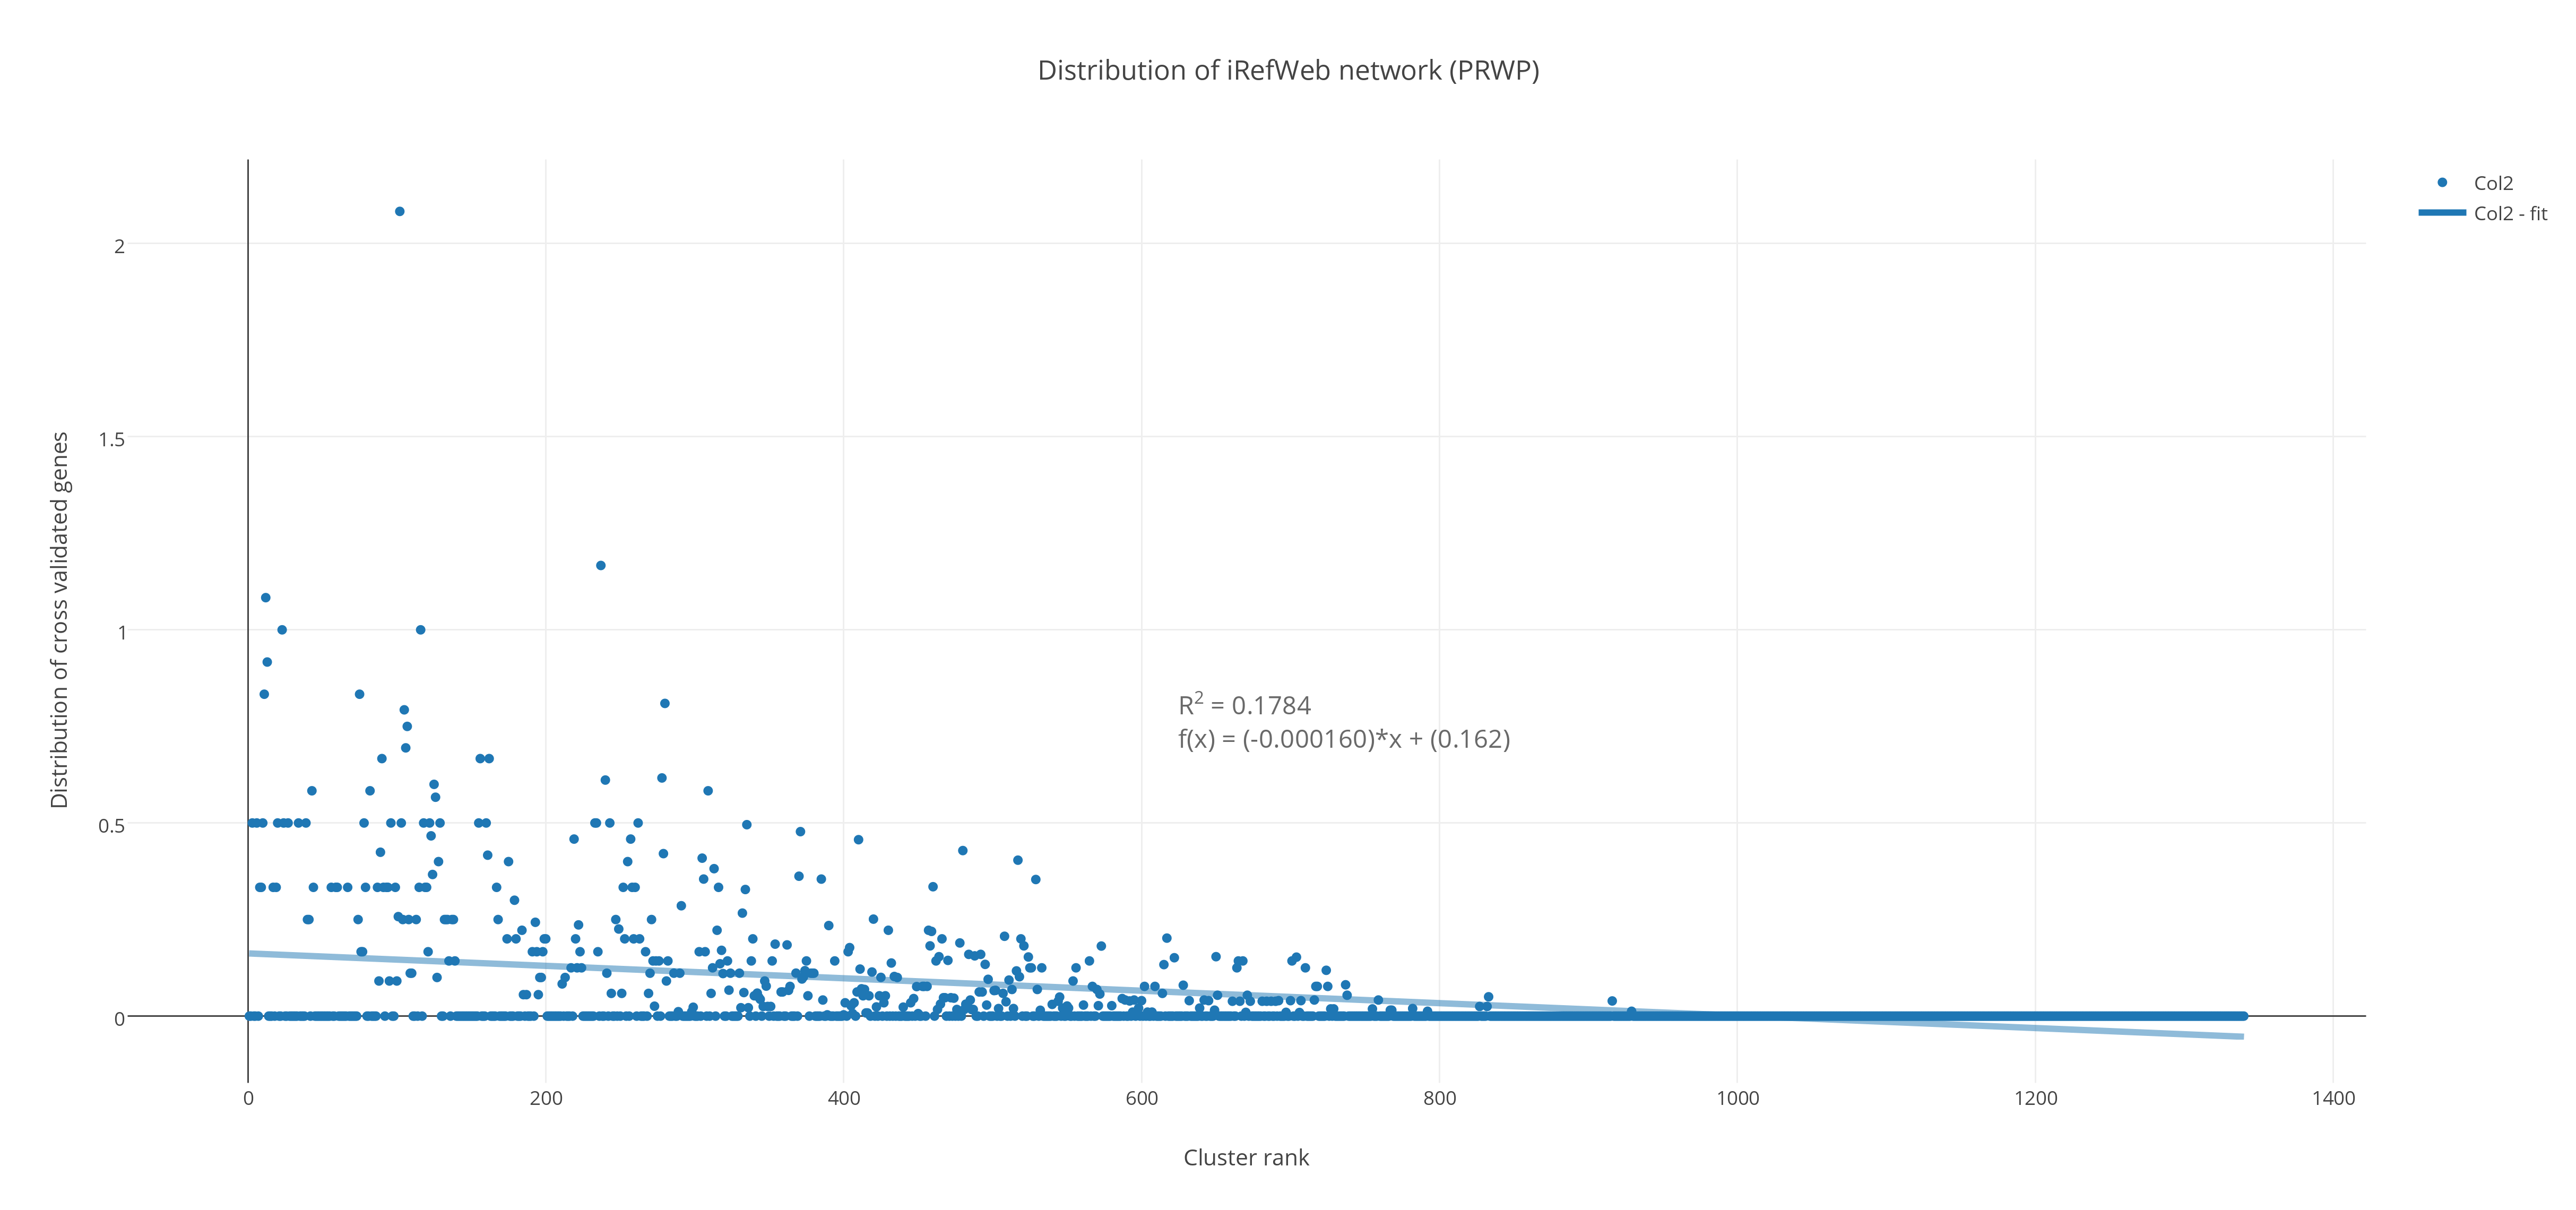
\includegraphics[width=15cm]{Distribution_of_iRefWeb_network_PRWP}
\end{figure}
\begin{figure}
    \label{fig:irefweb-maa}
    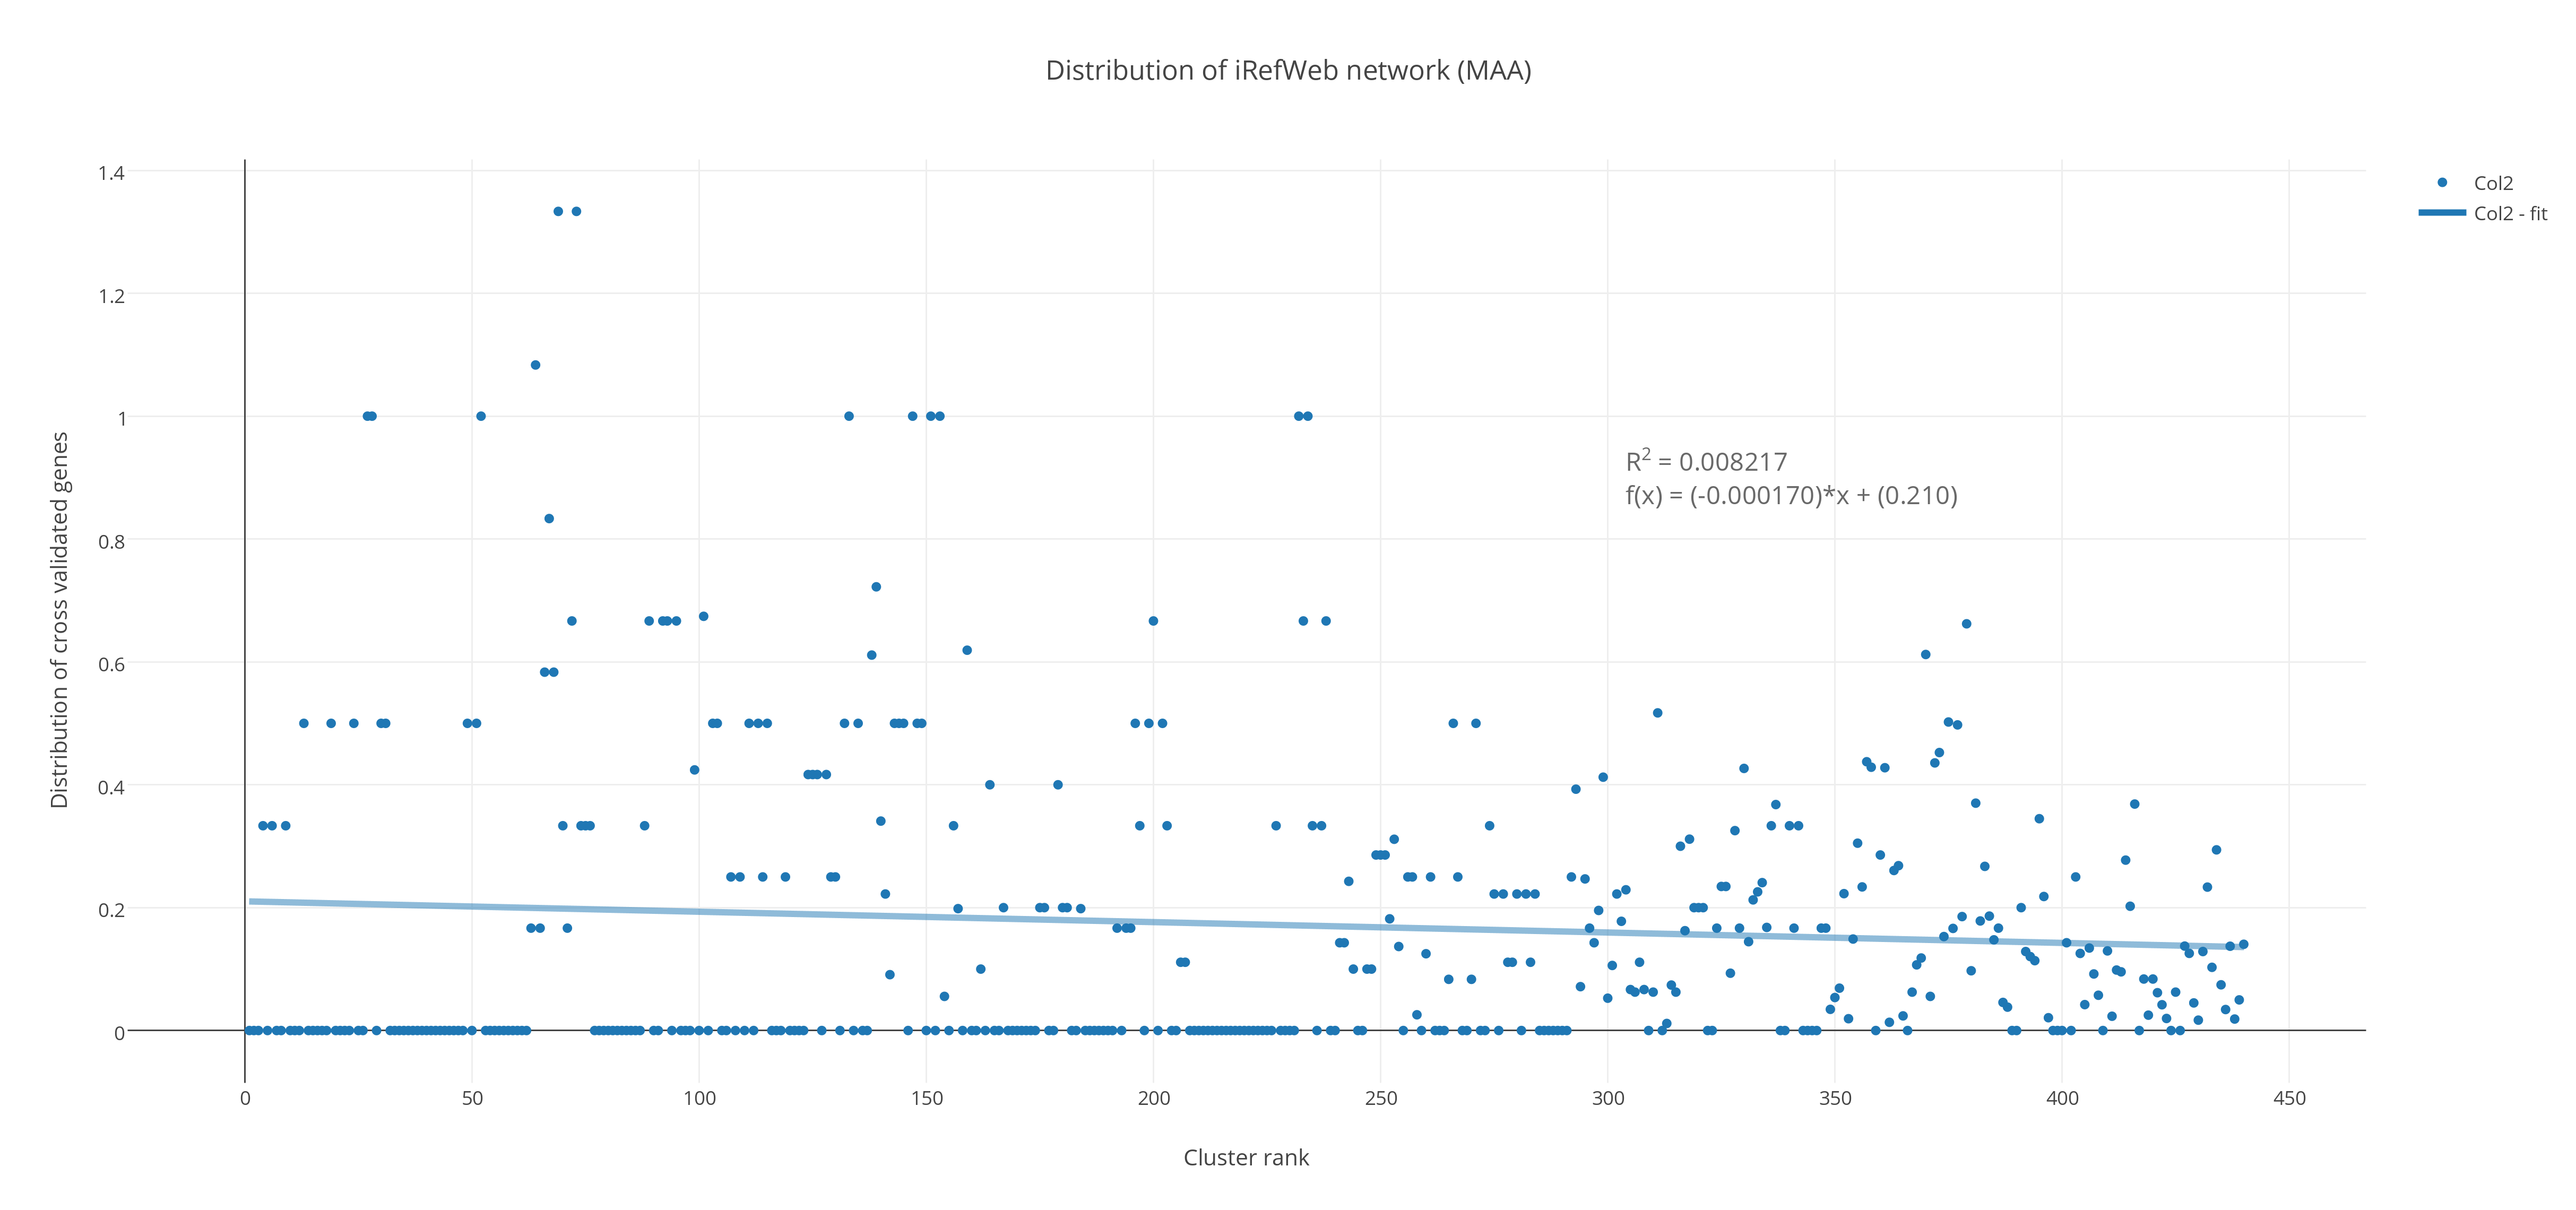
\includegraphics[width=15cm]{Distribution_of_iRefWeb_network_MAA}
\end{figure}
\begin{figure}
    \label{fig:cosmic-prwp}
    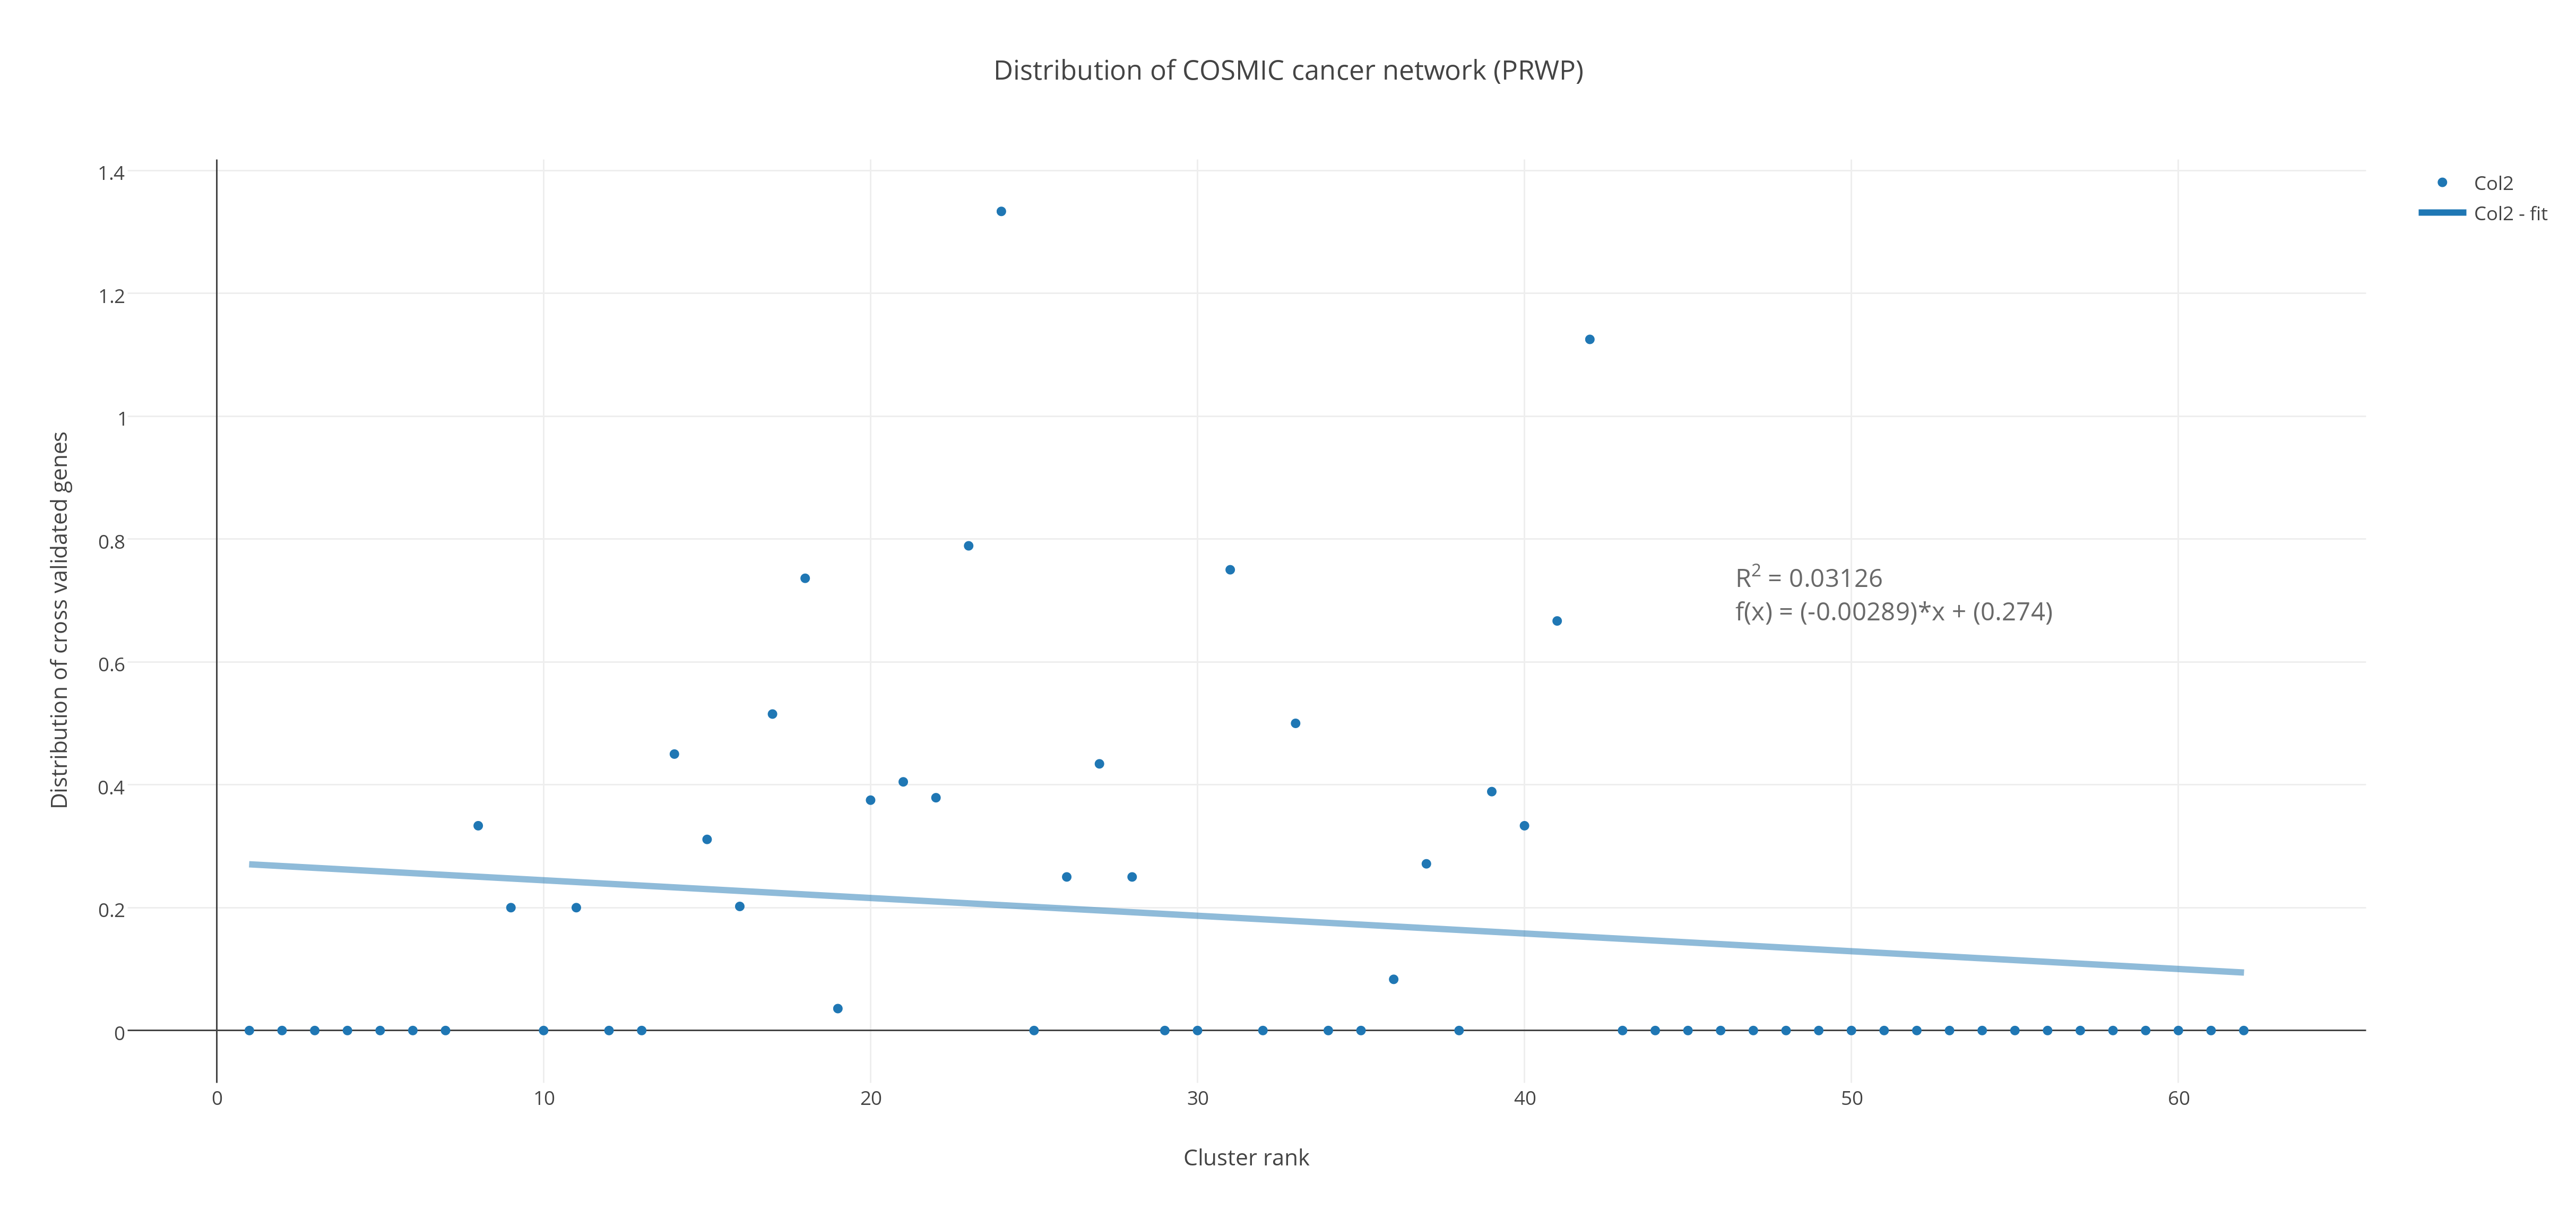
\includegraphics[width=15cm]{Distribution_of_COSMIC_cancer_network_PRWP}
\end{figure}
\begin{figure}
    \label{fig:cosmic-maa}
    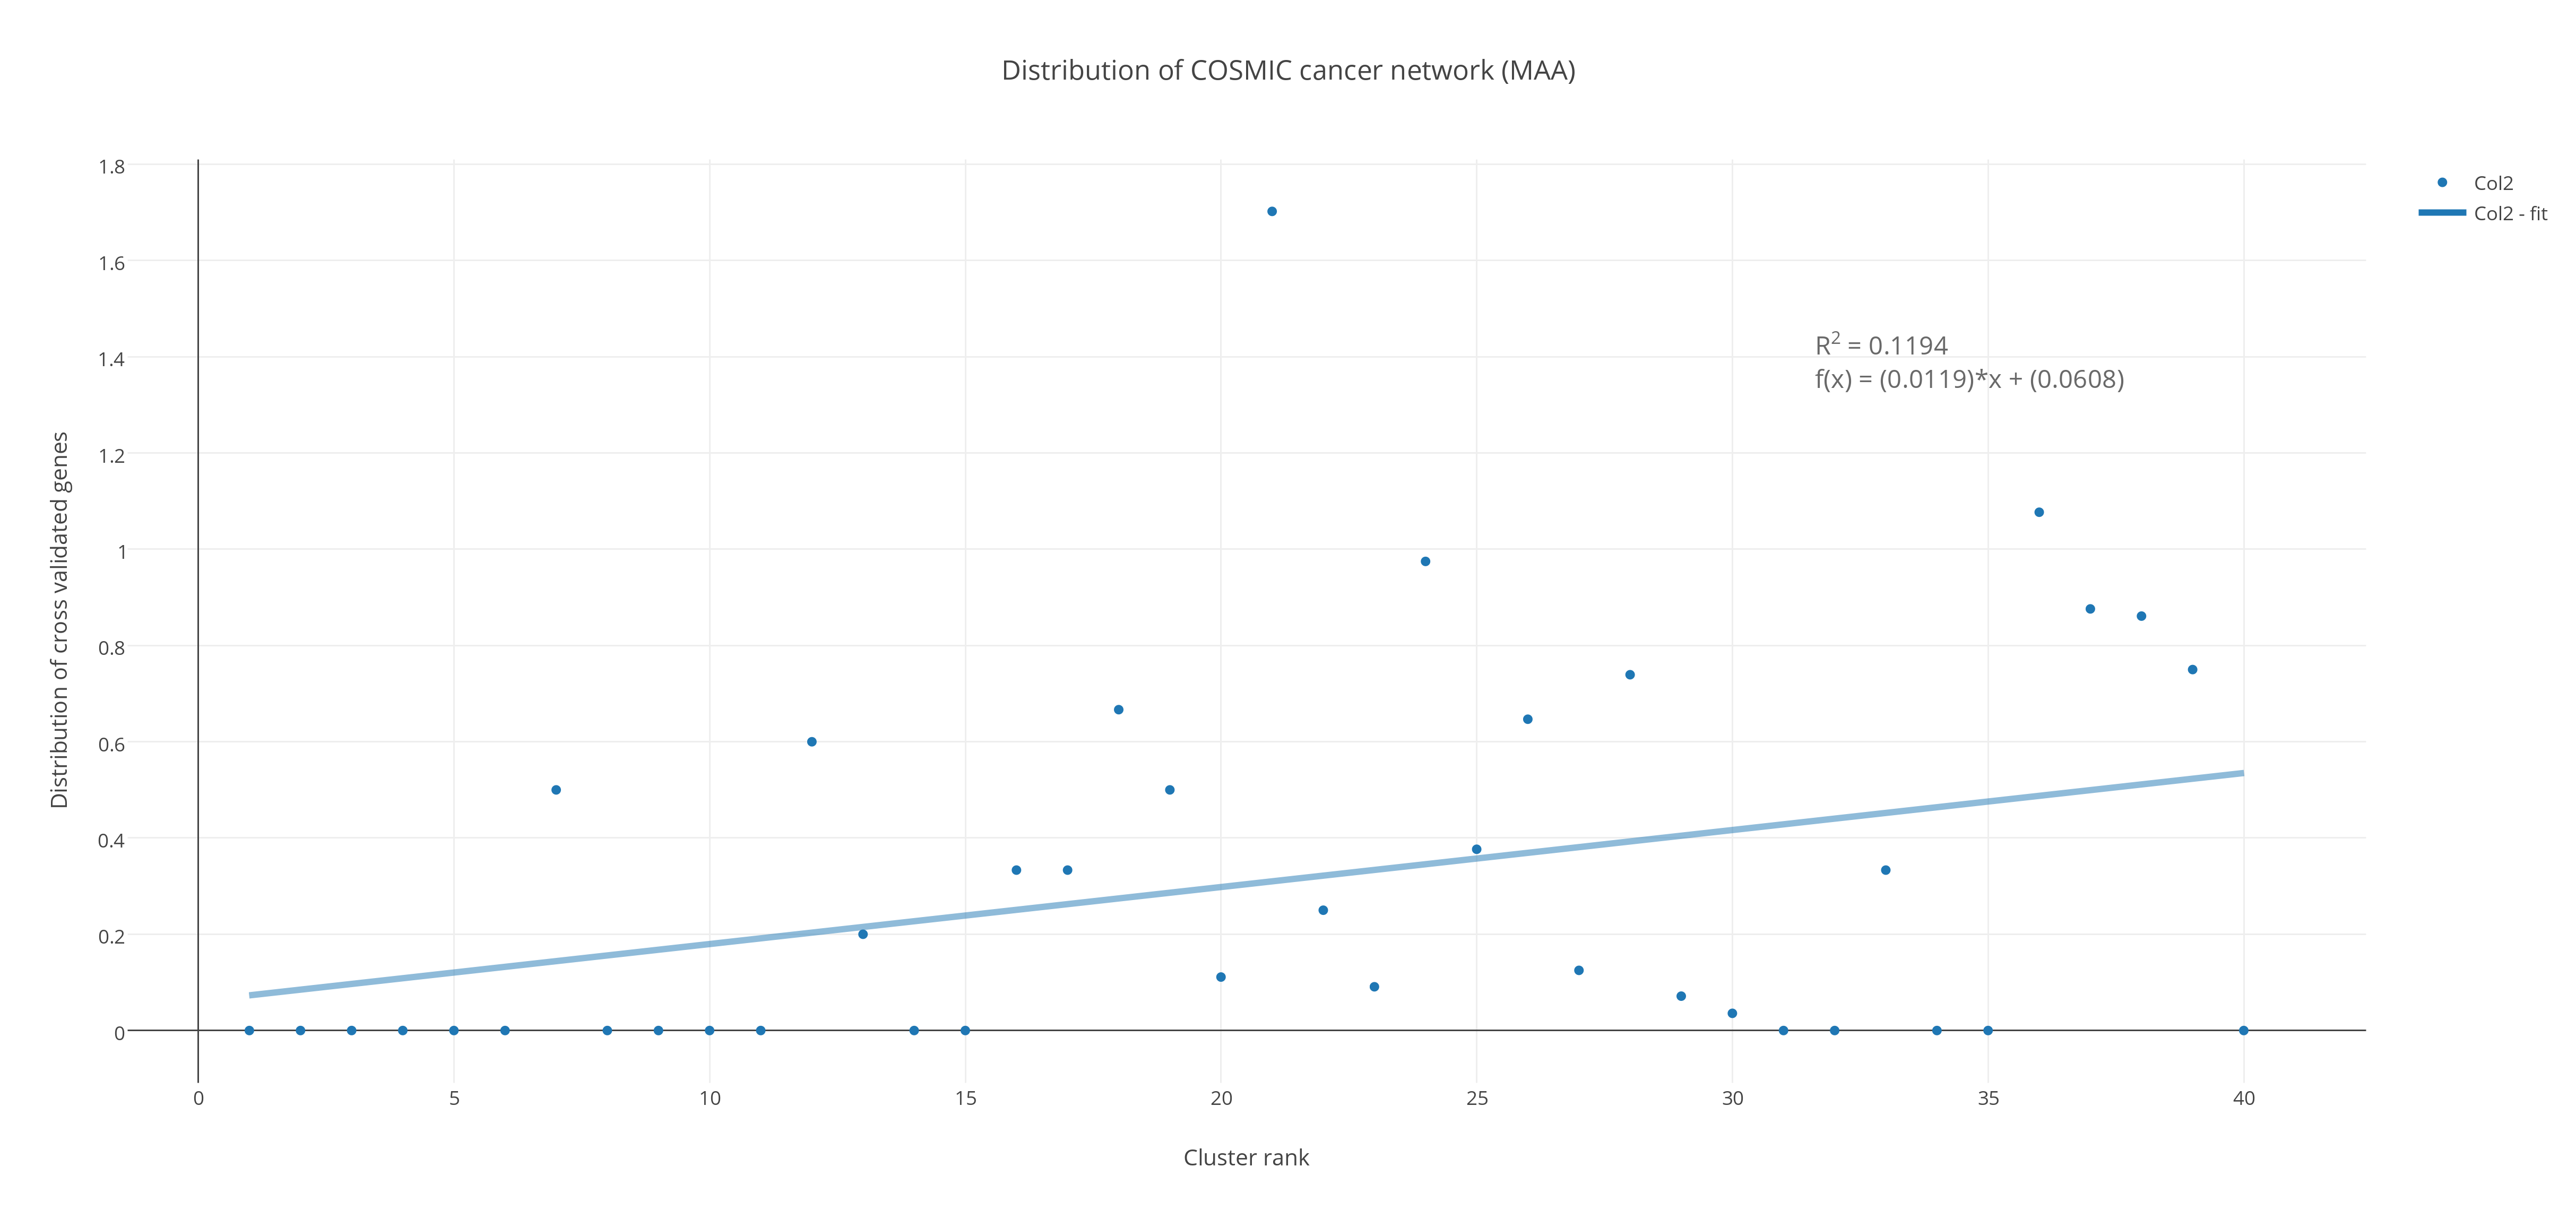
\includegraphics[width=15cm]{Distribution_of_COSMIC_cancer_network_MAA}
\end{figure}

\section{Jensen comparison}
%\begin{figure}
%    \label{fig:txt-irefweb-prwp}
%    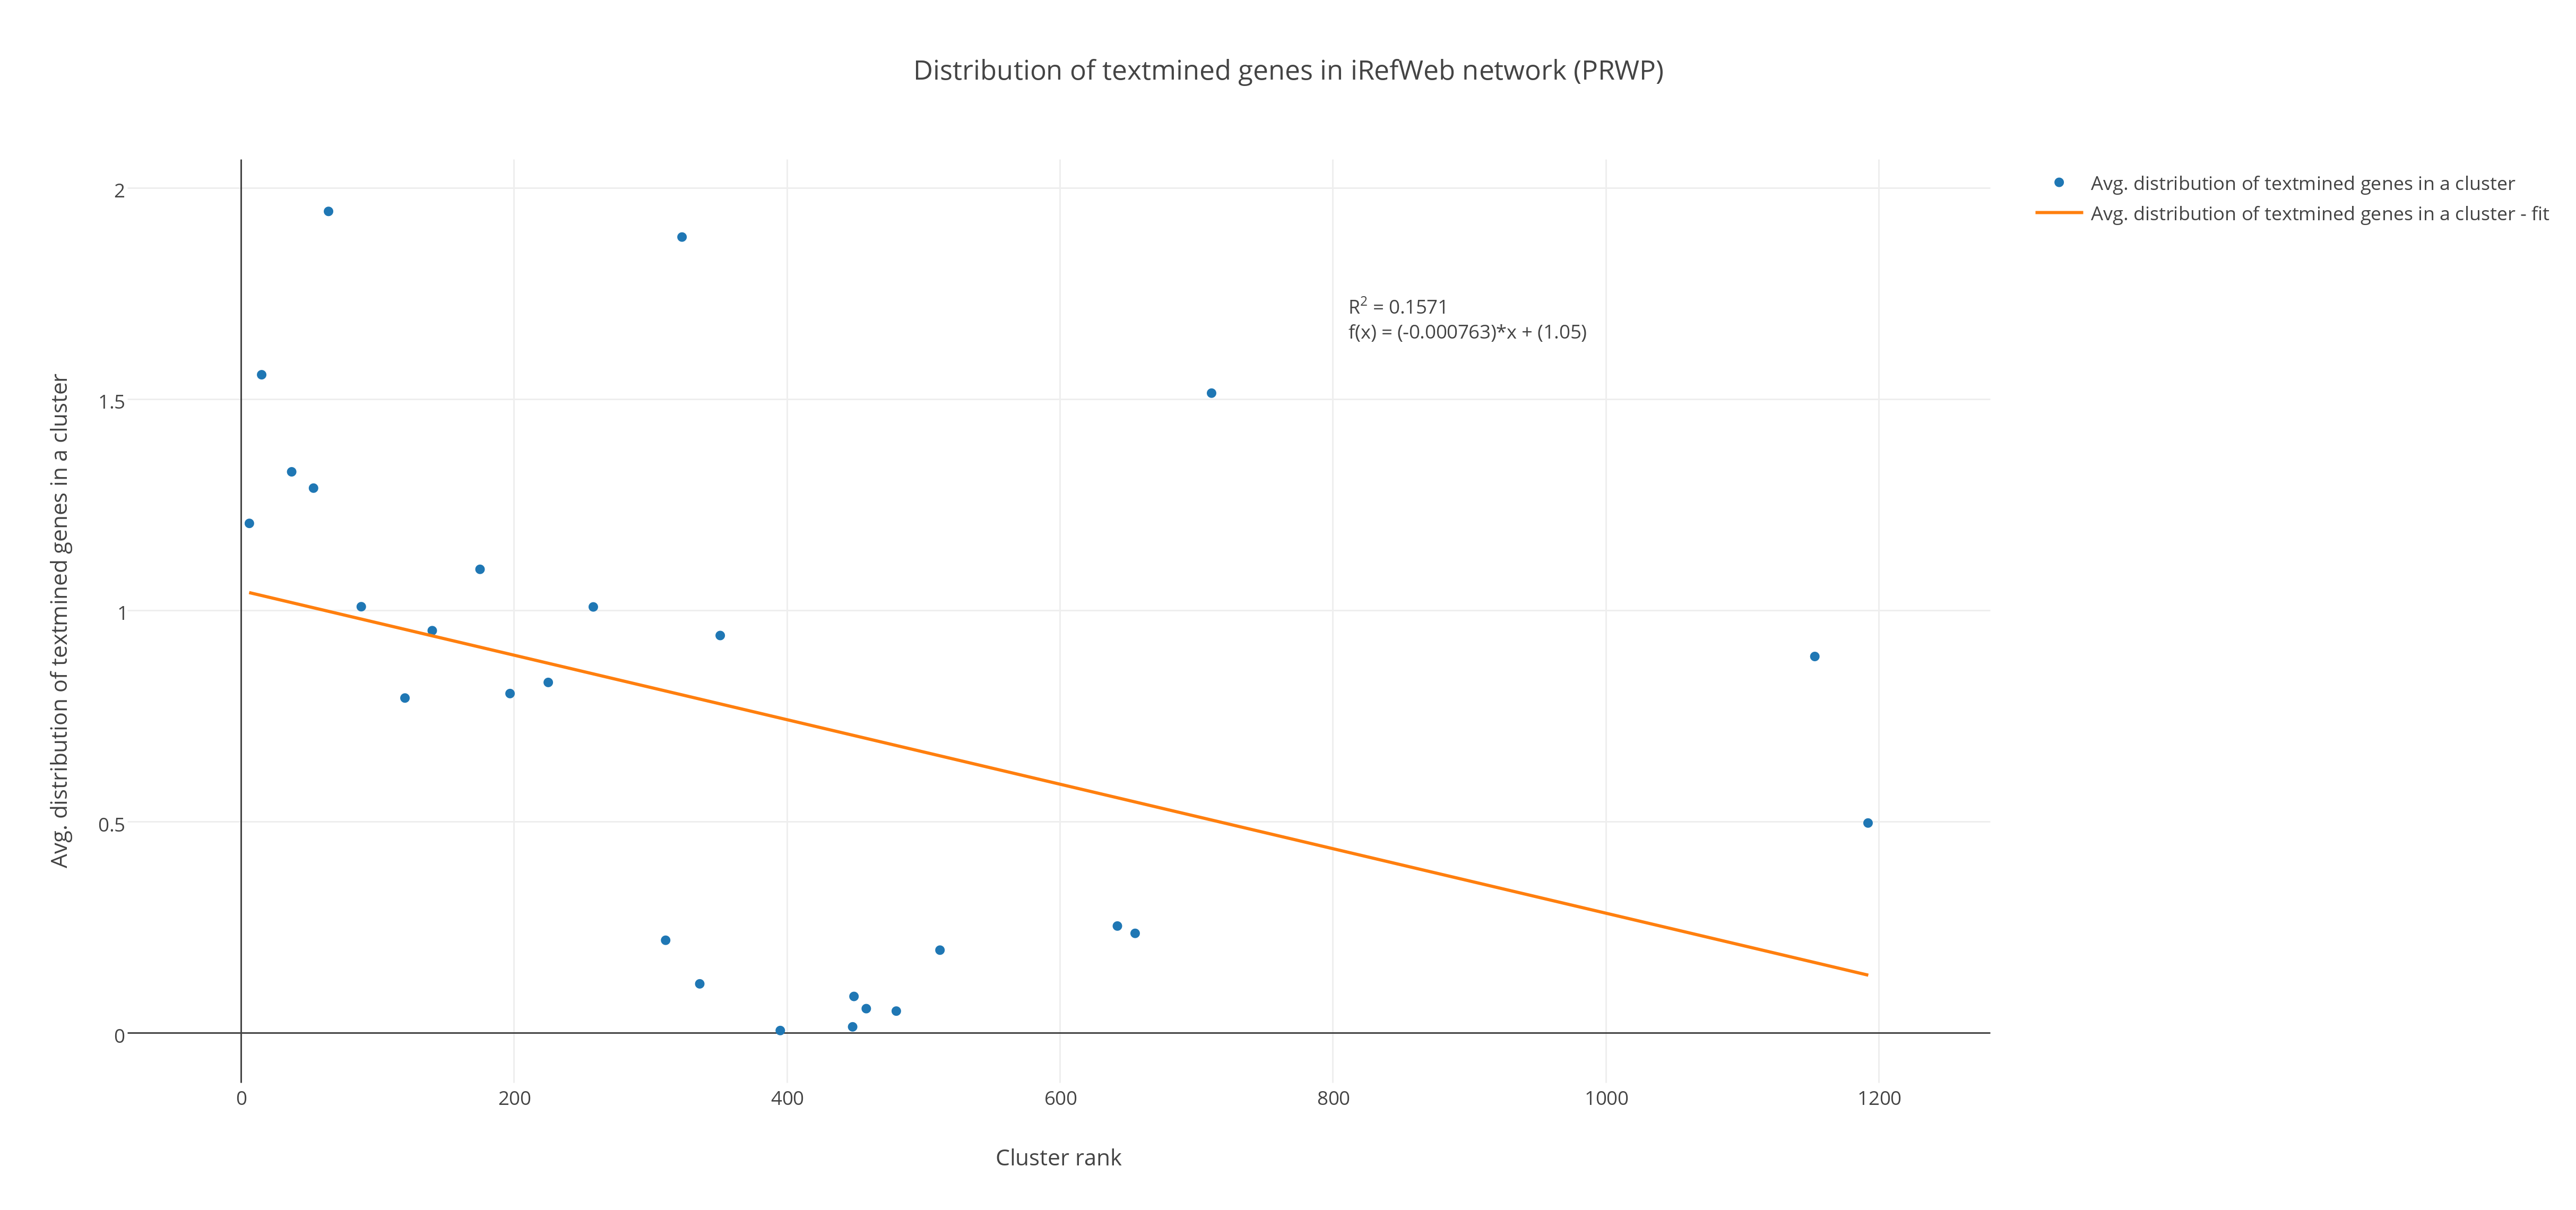
\includegraphics[width=15cm]{Distribution_of_textmined_genes_in_iRefWeb_network_PRWP}
%\end{figure}
%\begin{figure}
%    \label{fig:txt-irefweb-maa}
%    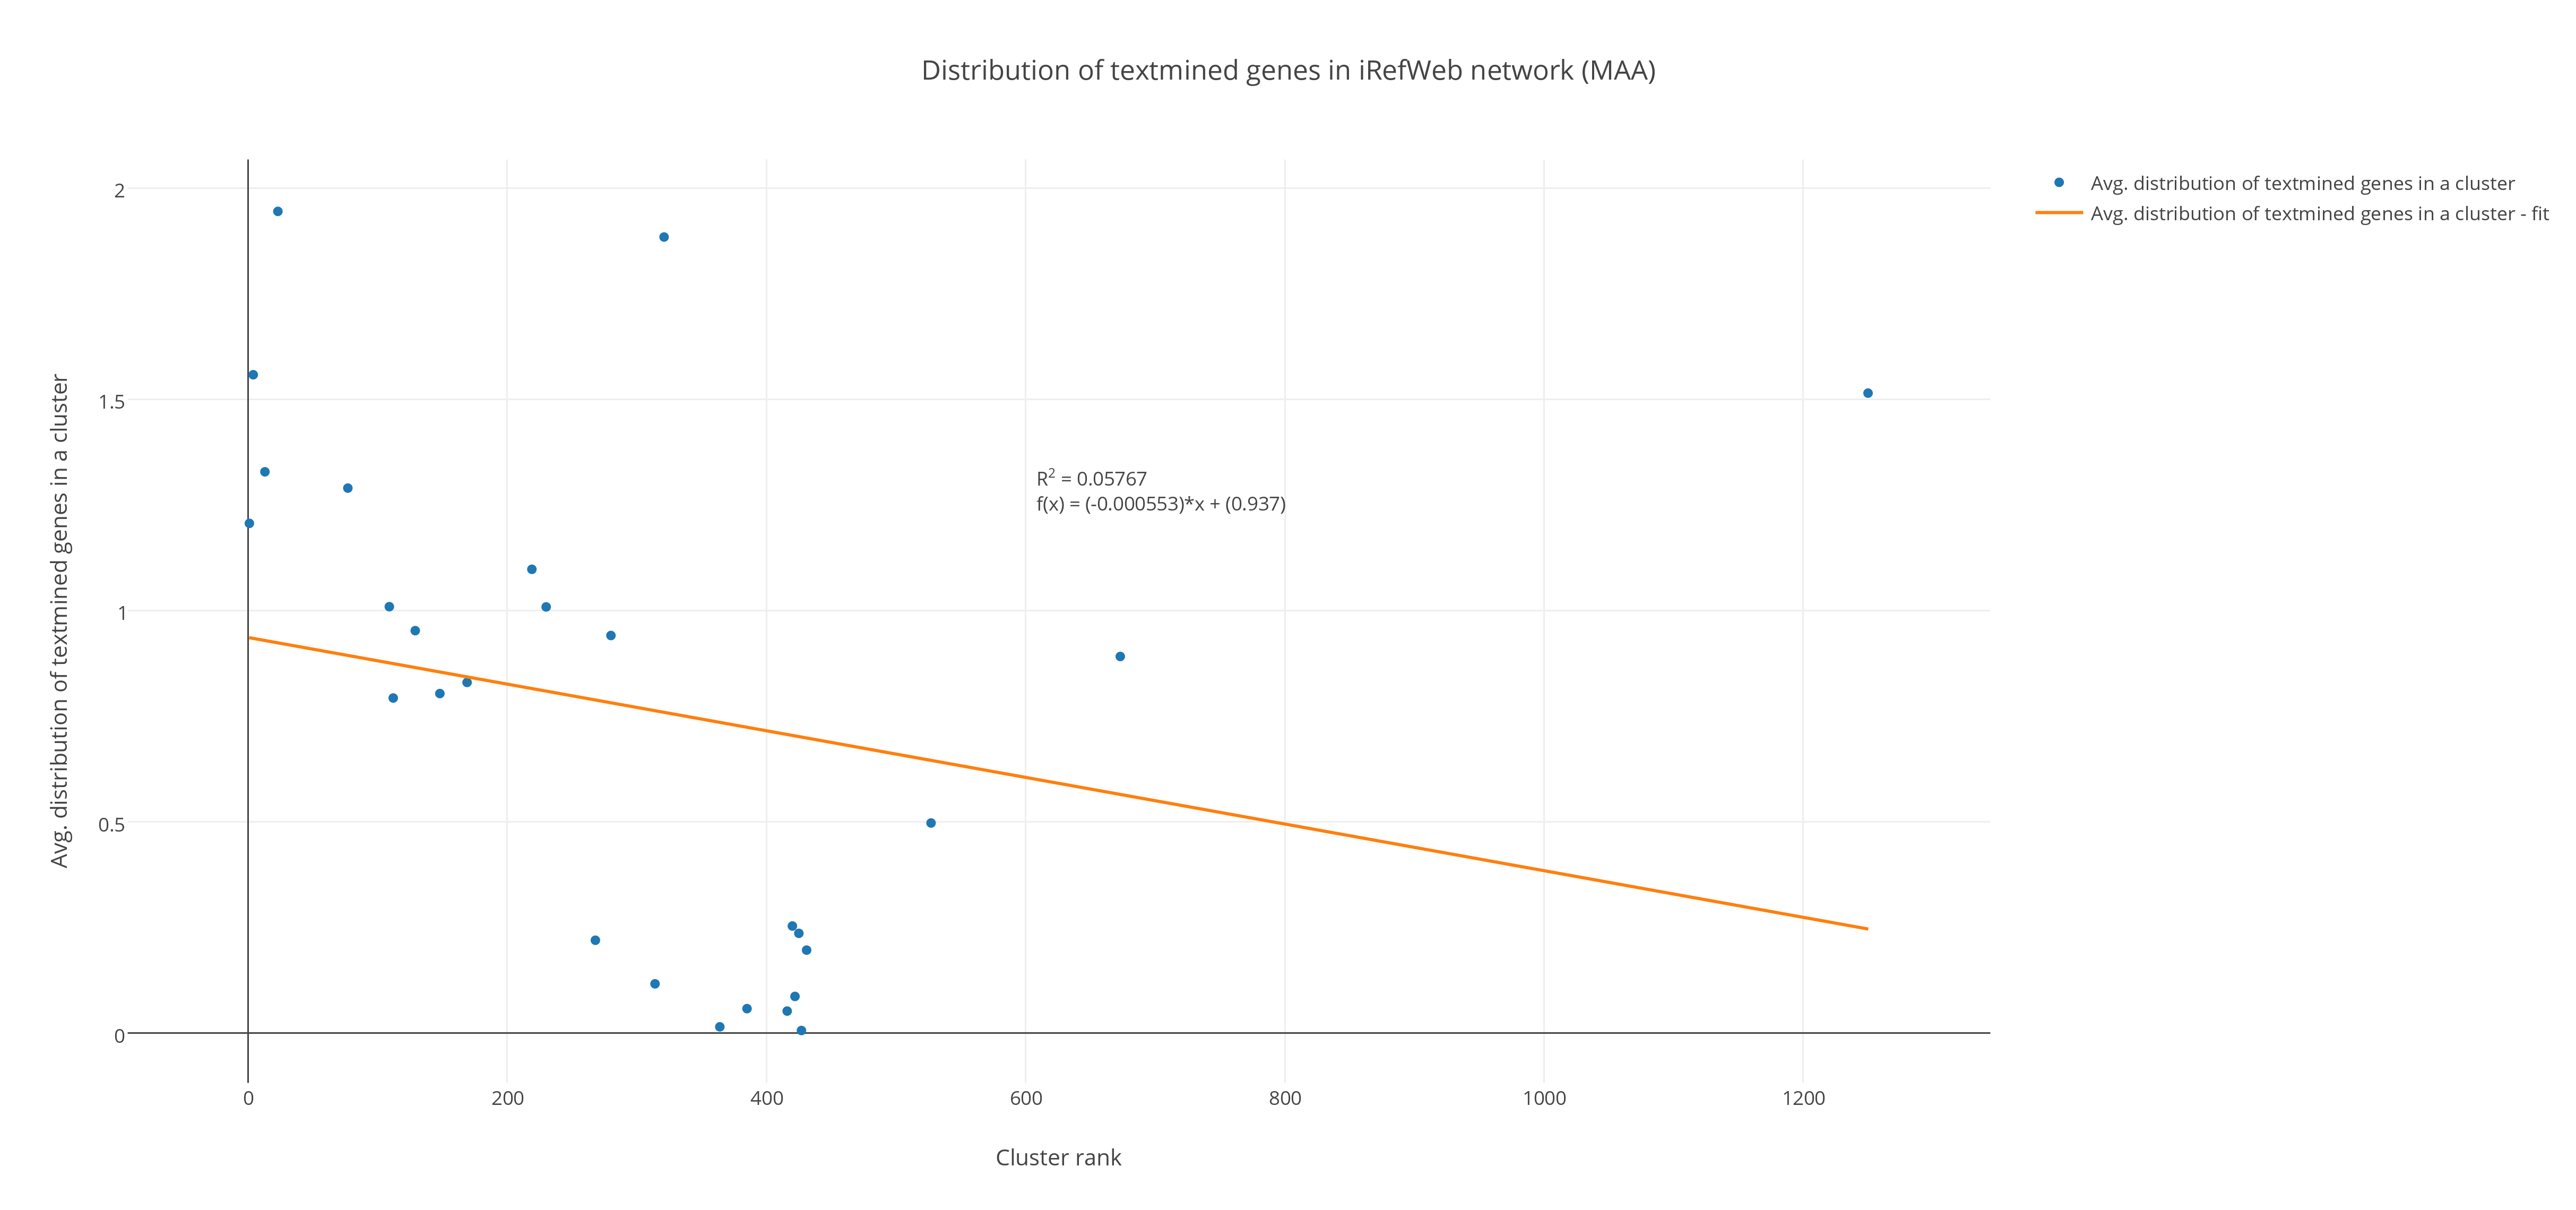
\includegraphics[width=15cm]{Distribution_of_textmined_genes_in_iRefWeb_network_MAA}
%\end{figure}
%\begin{figure}
%    \label{fig:know-irefweb-prwp}
%    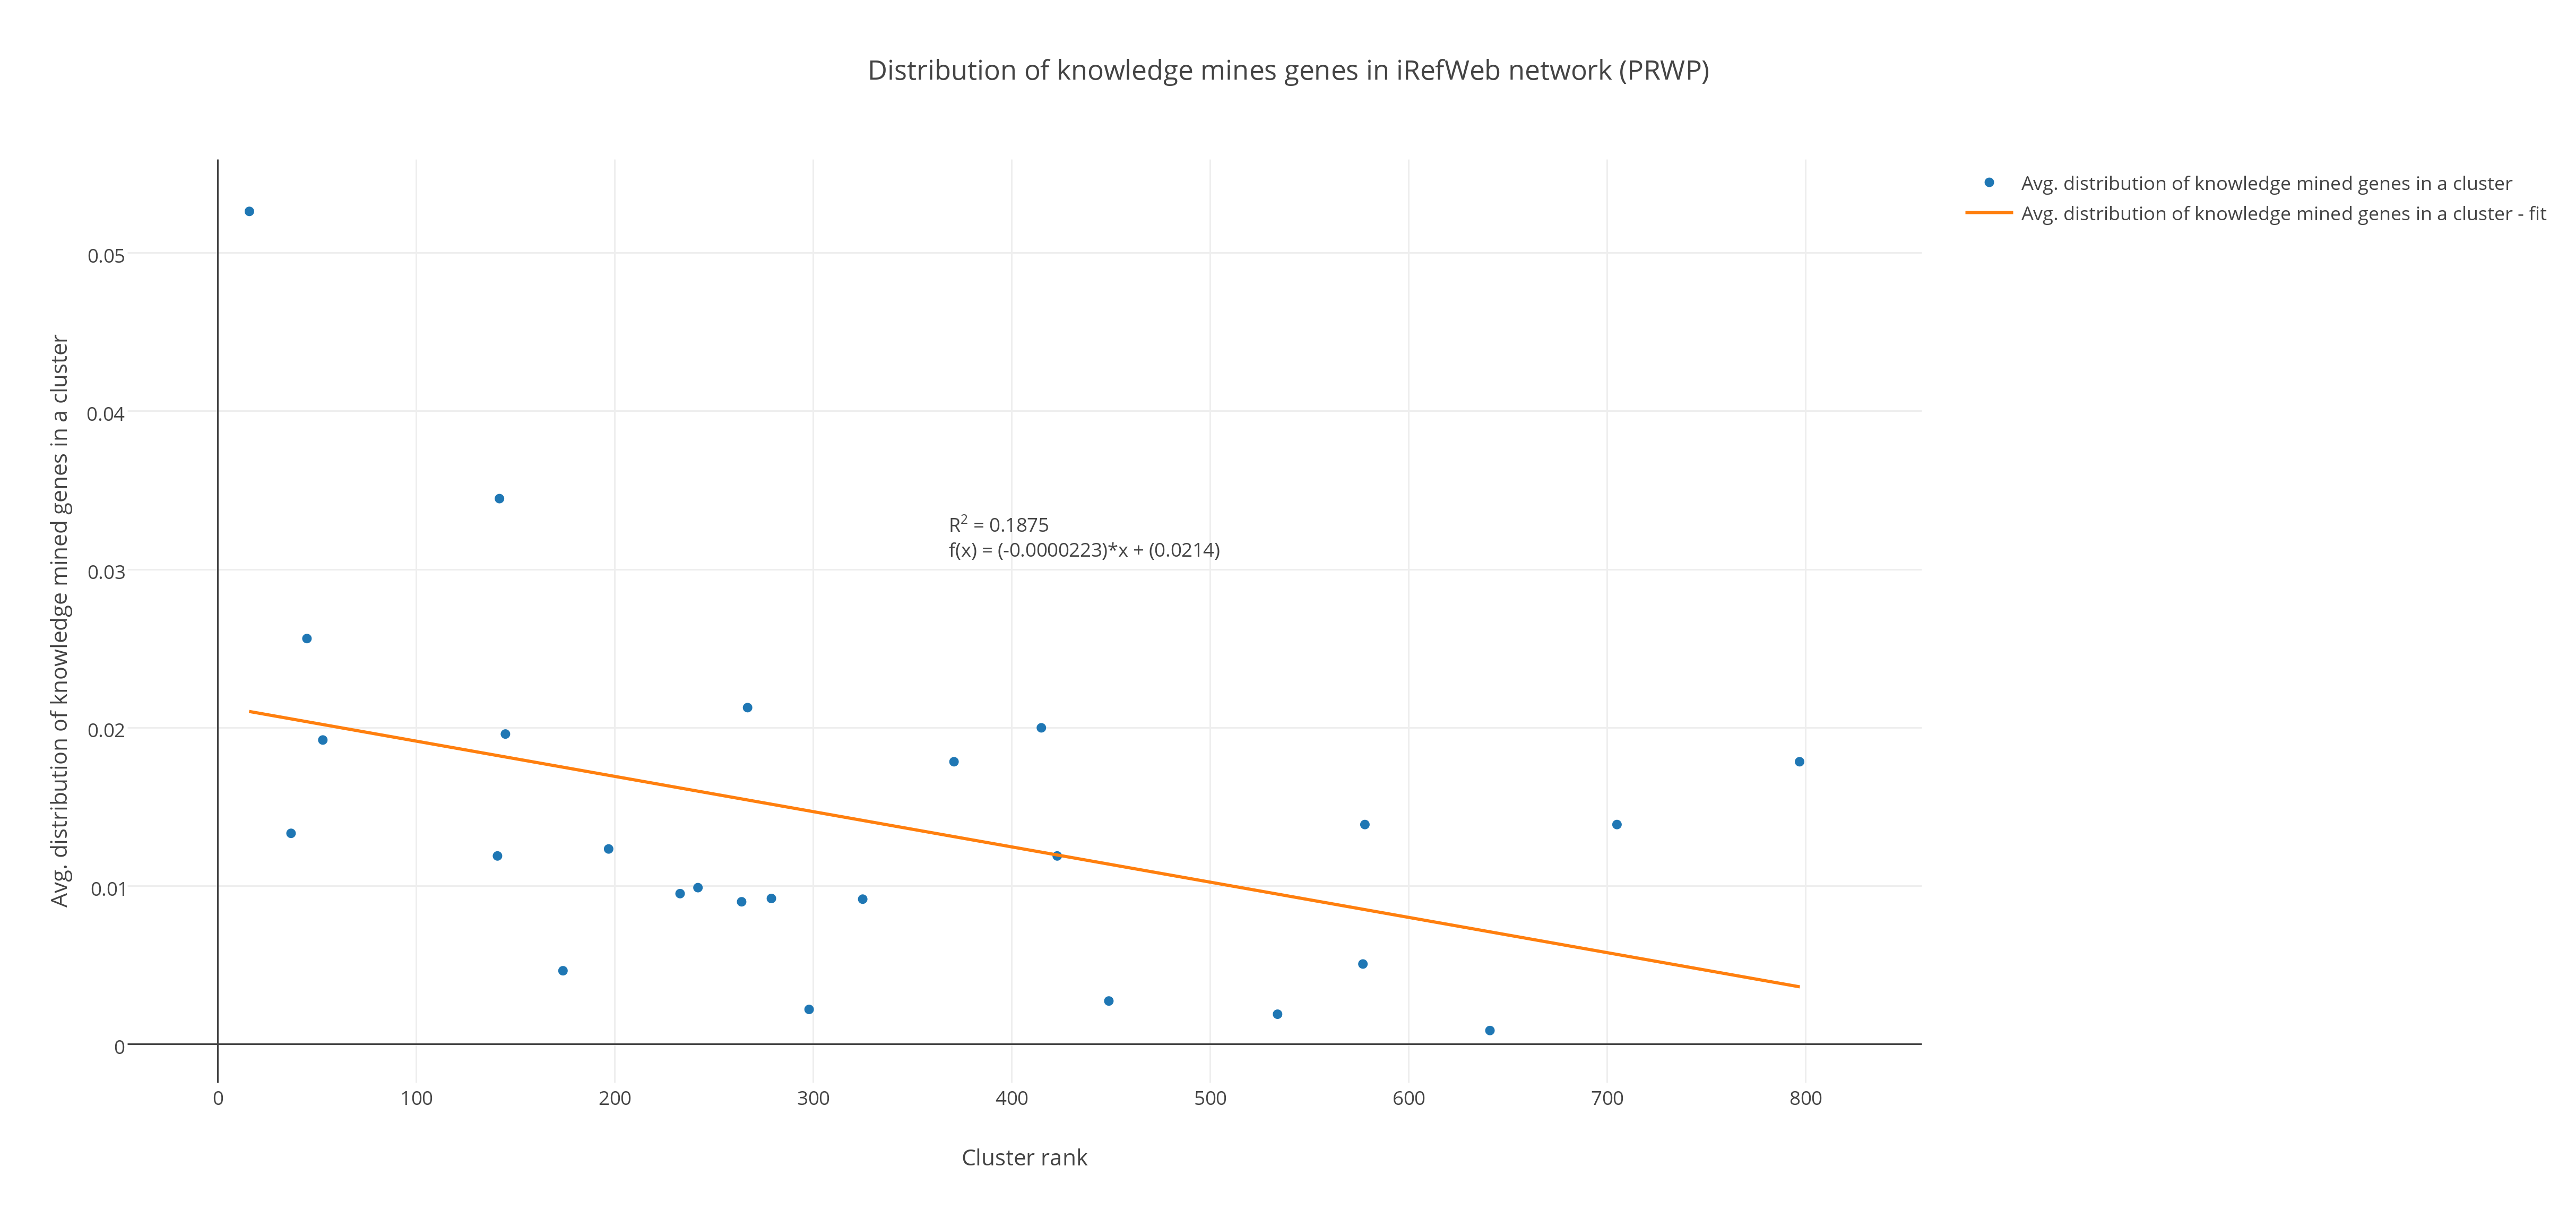
\includegraphics[width=15cm]{Distribution_of_knowledge_mined_genes_in_iRefWeb_network_PRWP}
%\end{figure}
%\begin{figure}
%    \label{fig:know-irefweb-maa}
%    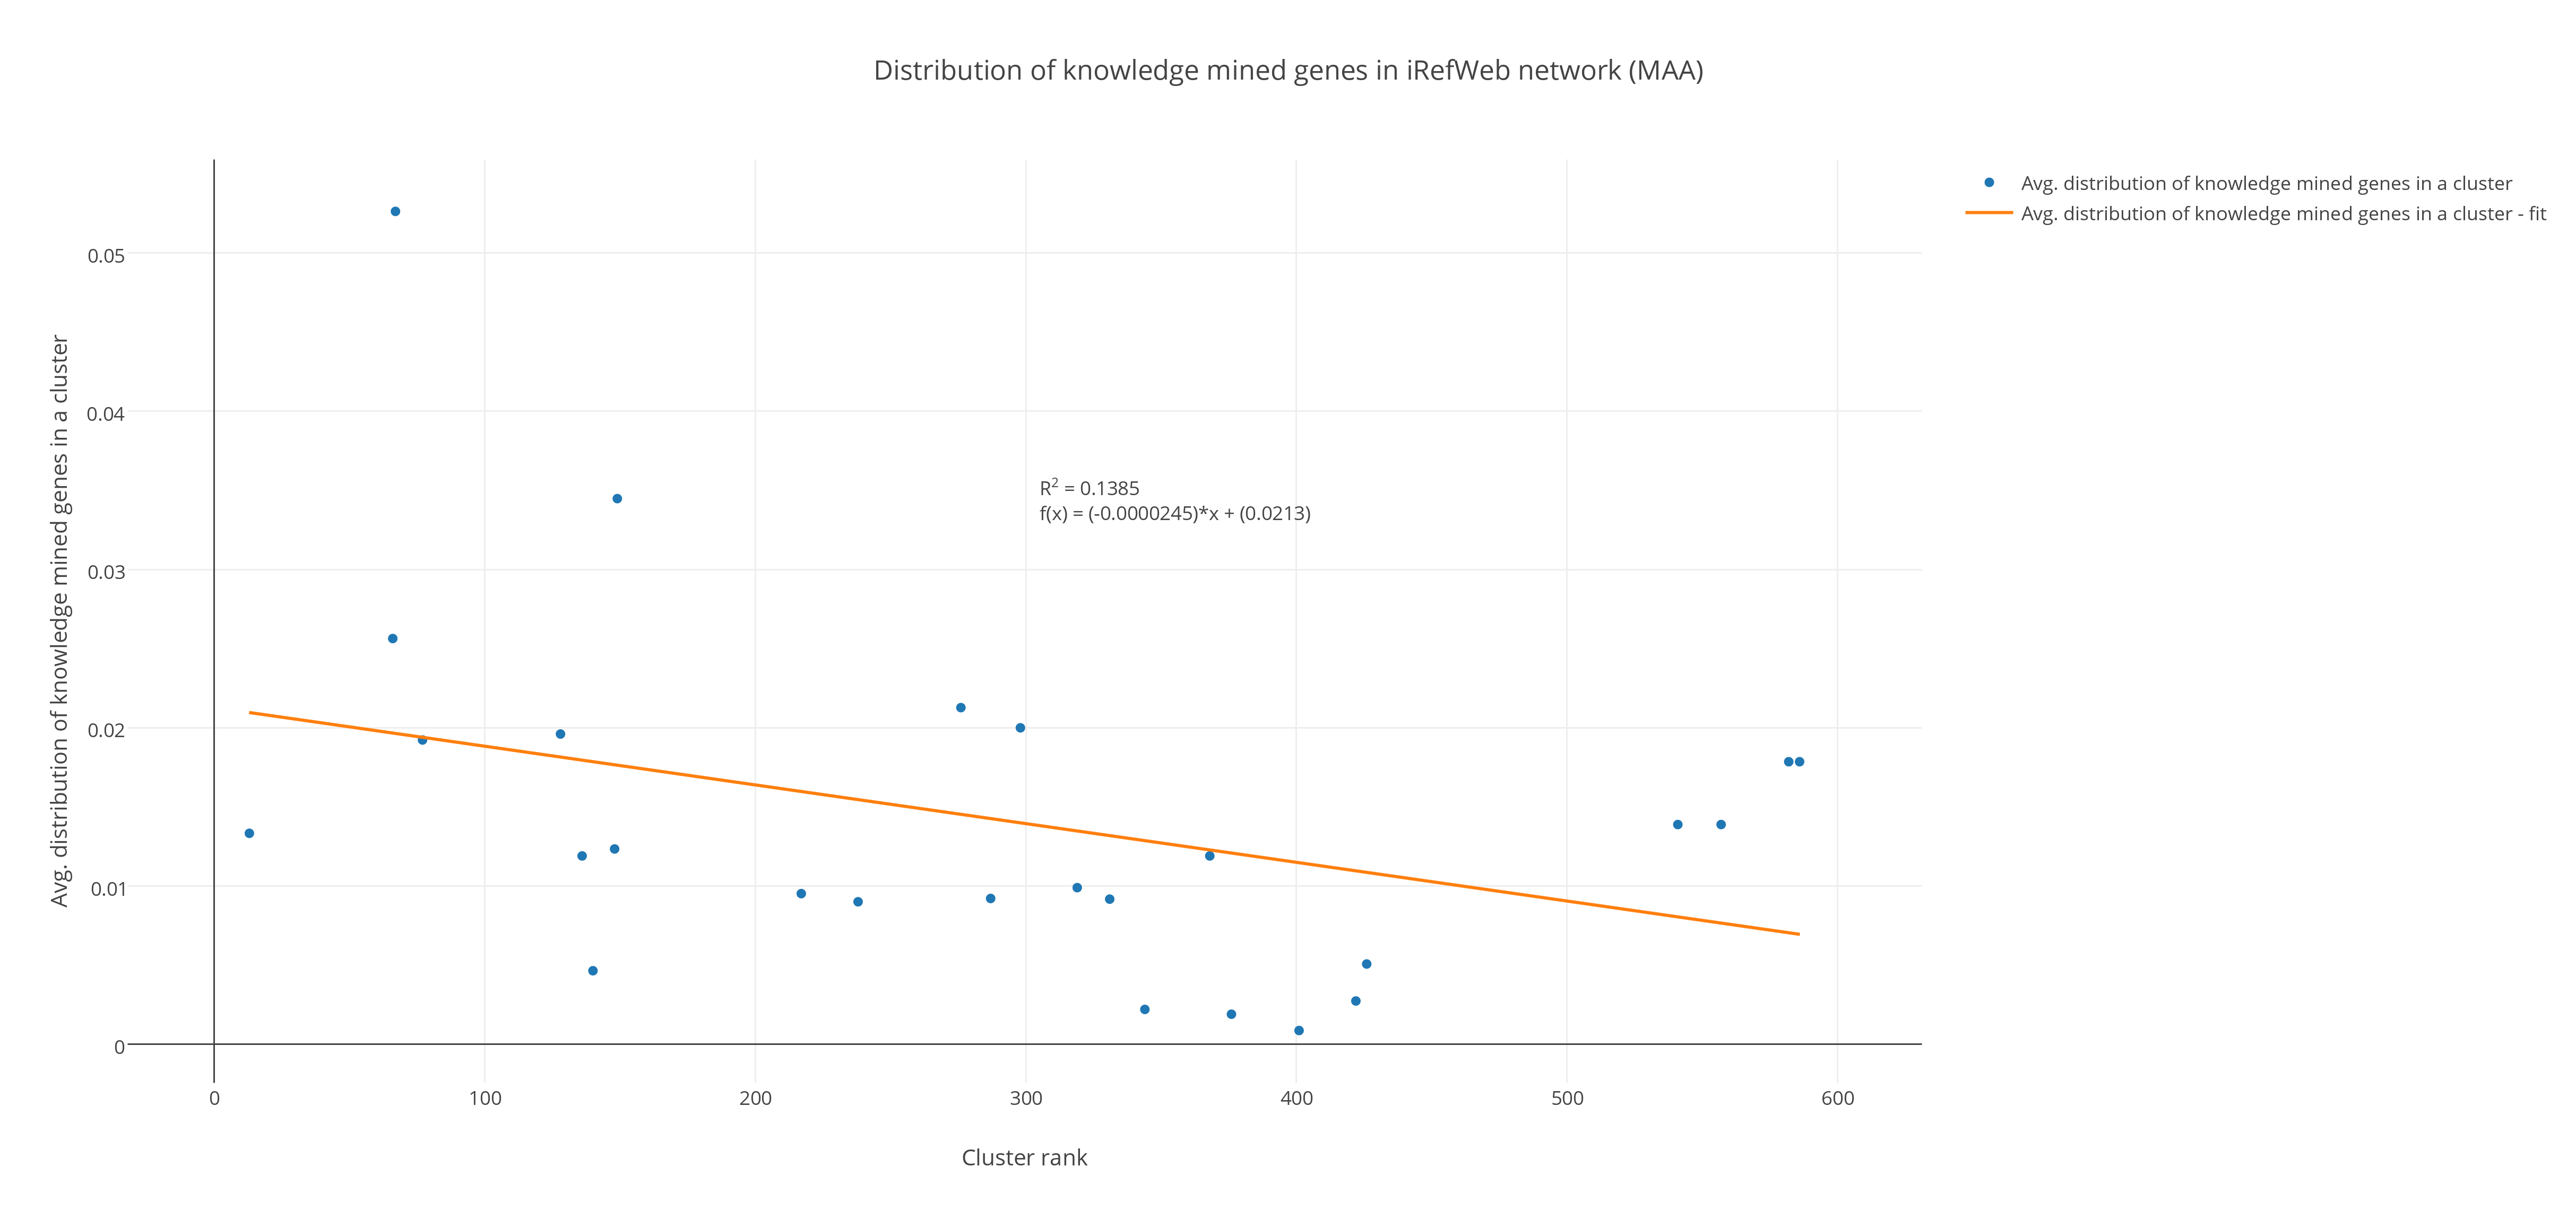
\includegraphics[width=15cm]{Distribution_of_knowledge_mined_genes_in_iRefWeb_network_MAA}
%\end{figure}
%\begin{figure}
%    \label{fig:exp-irefweb-prwp}
%    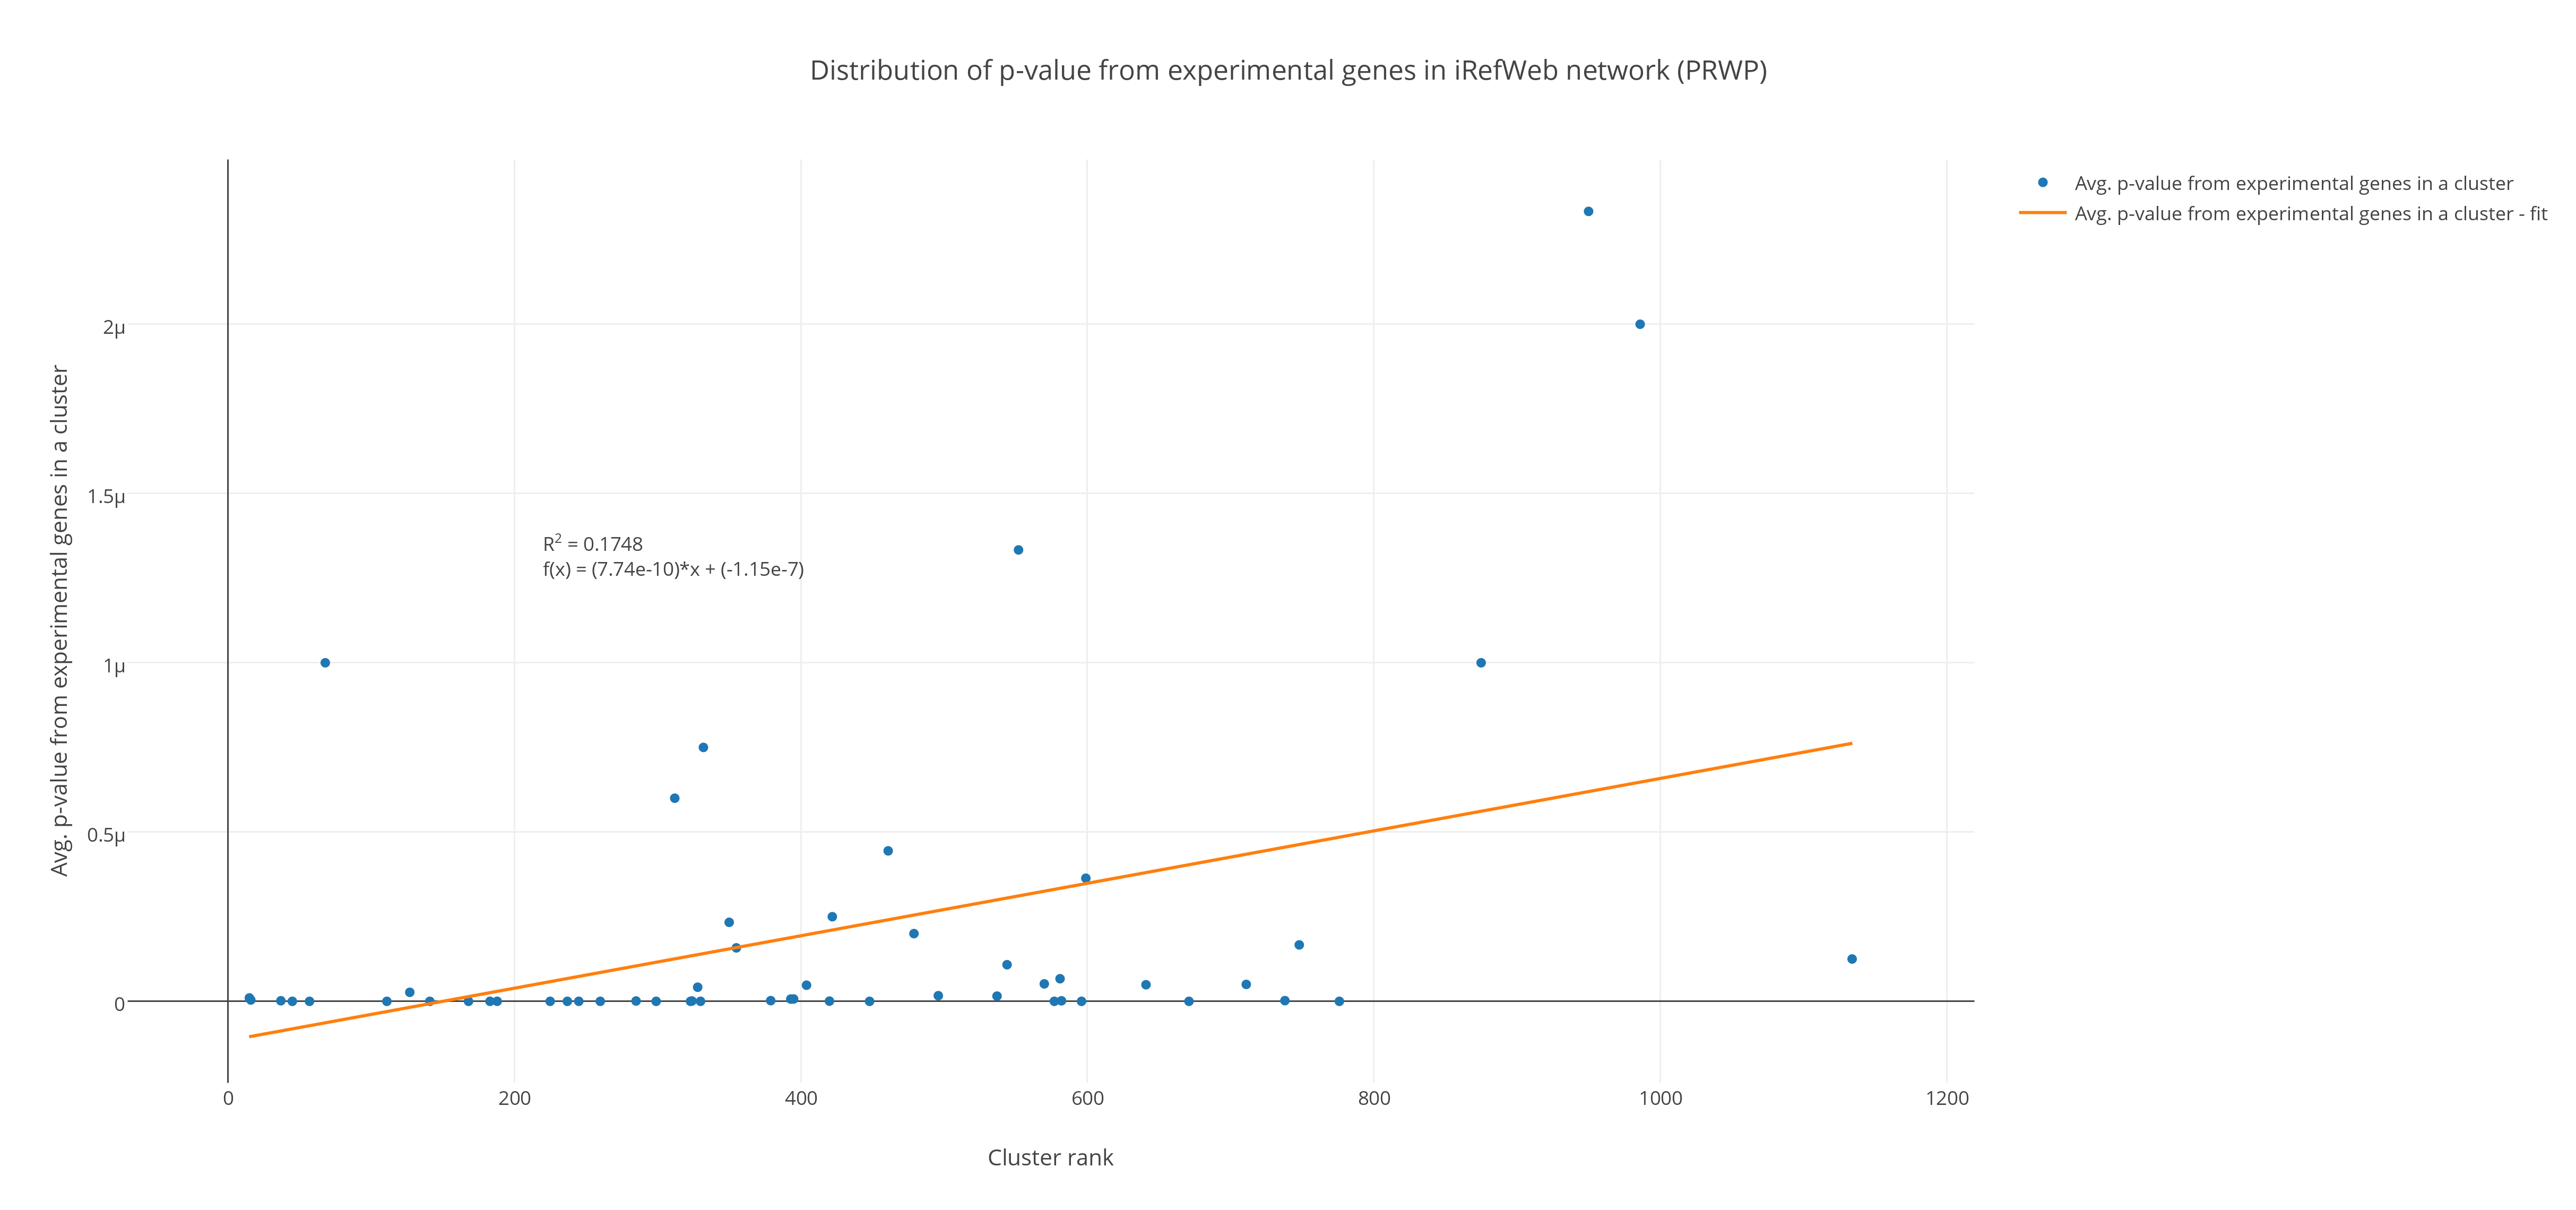
\includegraphics[width=15cm]{Distribution_of_p-value_from_experimental_genes_in_iRefWeb_network_PRWP}
%\end{figure}
%\begin{figure}
%    \label{fig:exp-irefweb-maa}
%    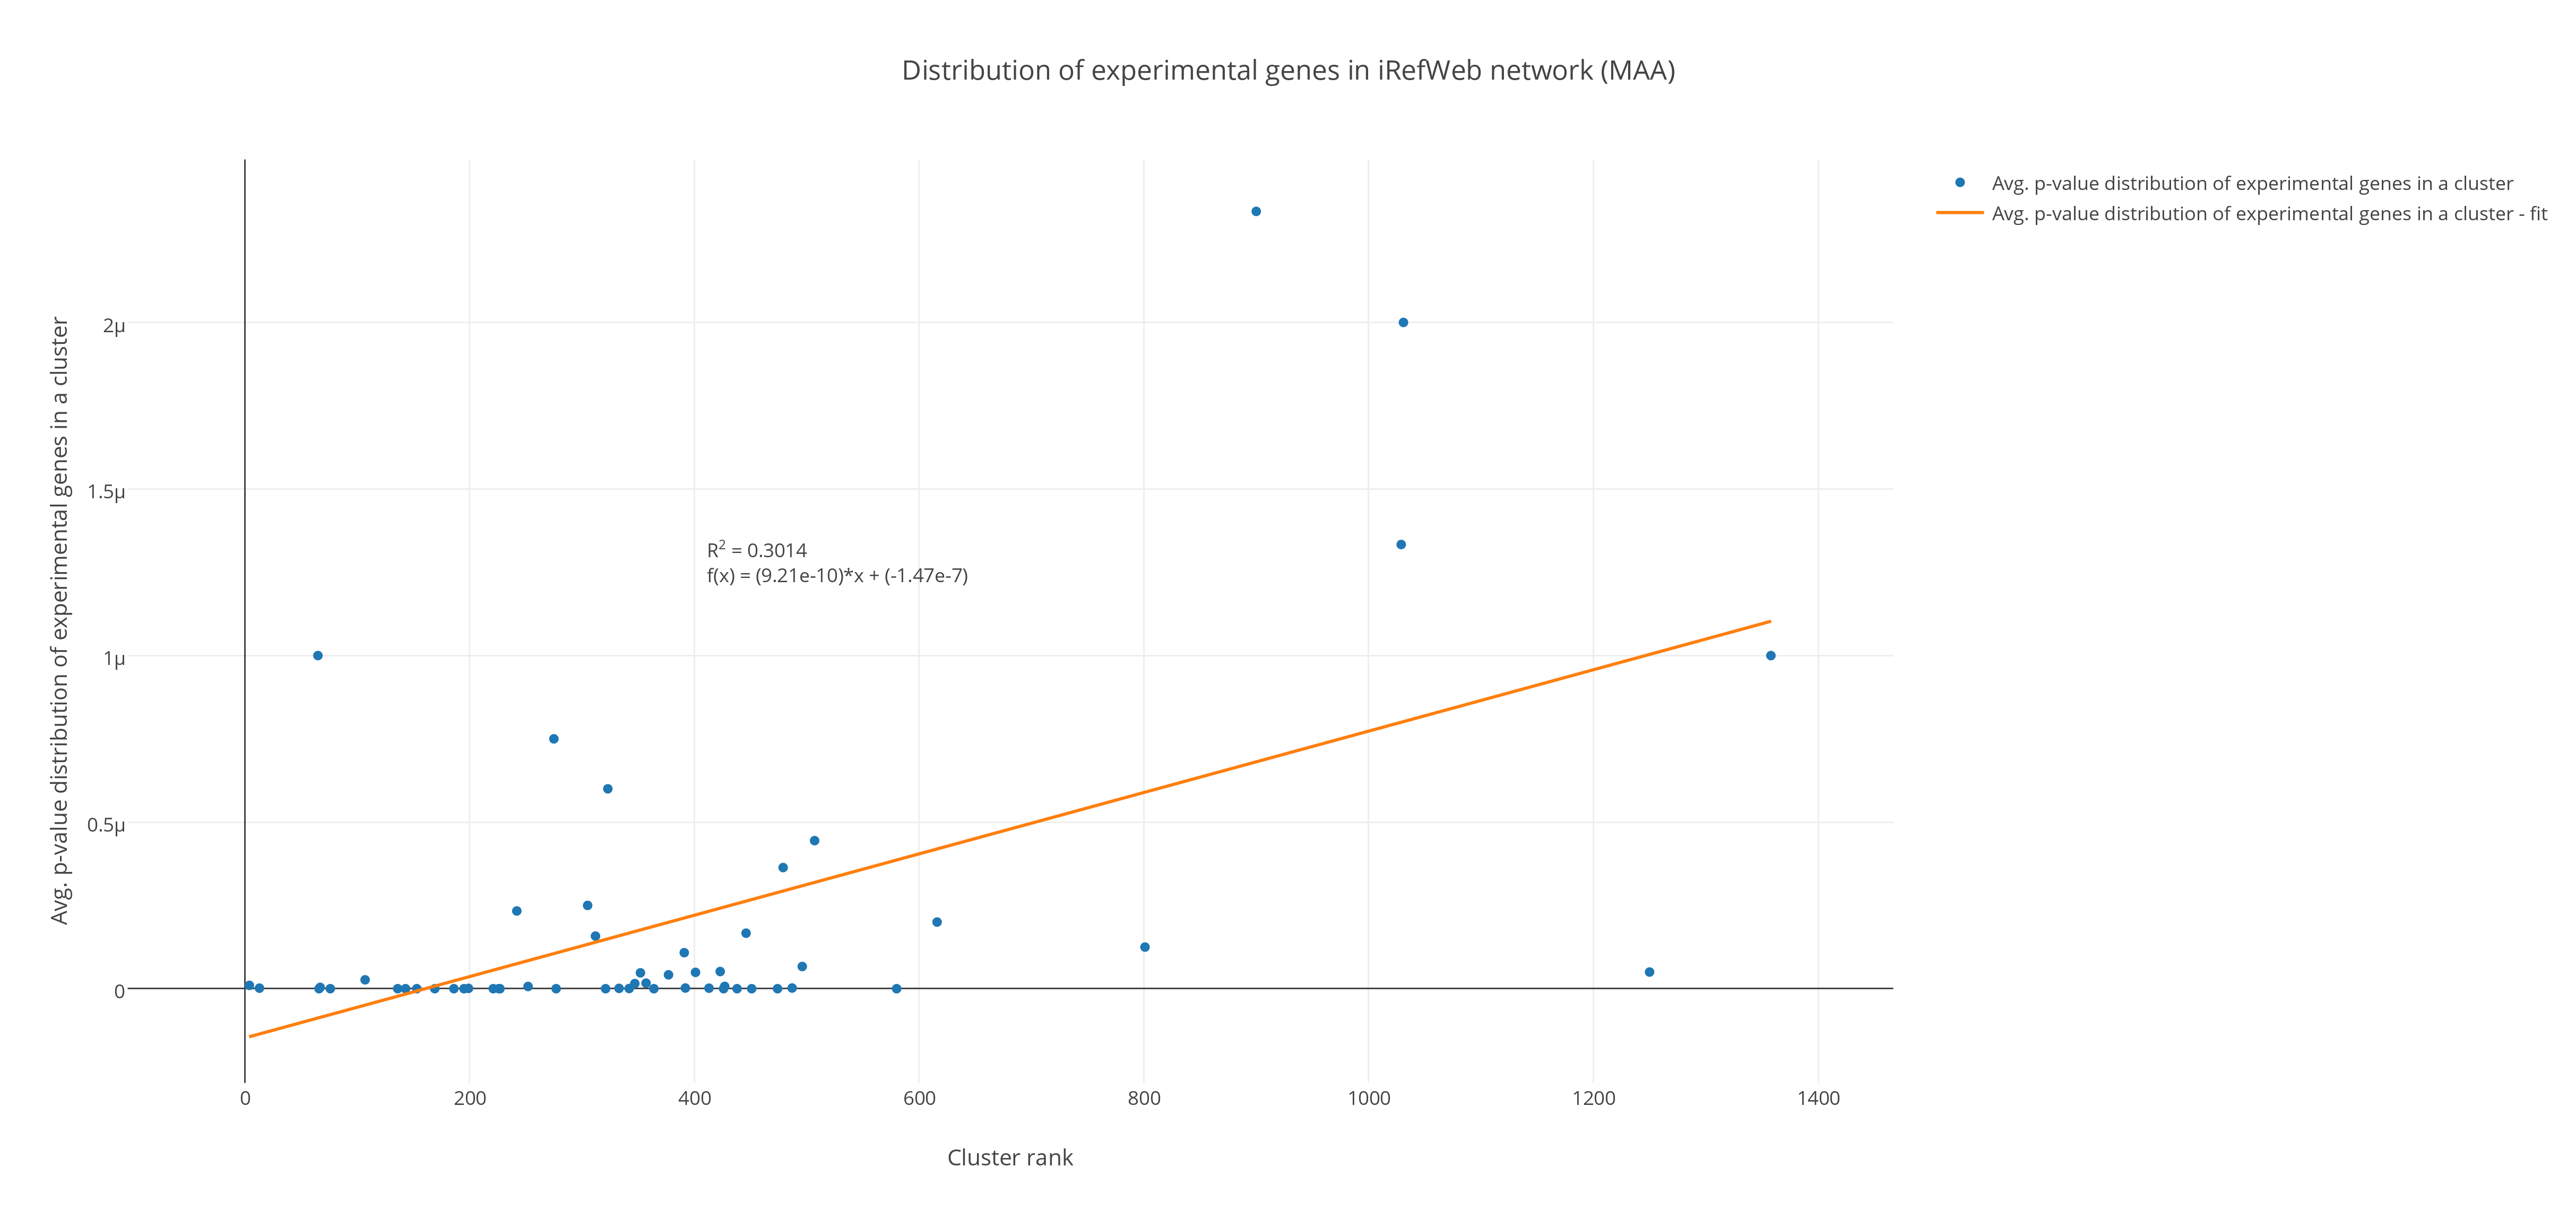
\includegraphics[width=15cm]{Distribution_of_experimental_genes_in_iRefWeb_network_MAA}
%\end{figure}
%\begin{figure}
%    \label{fig:txt-cosmic-prwp}
%    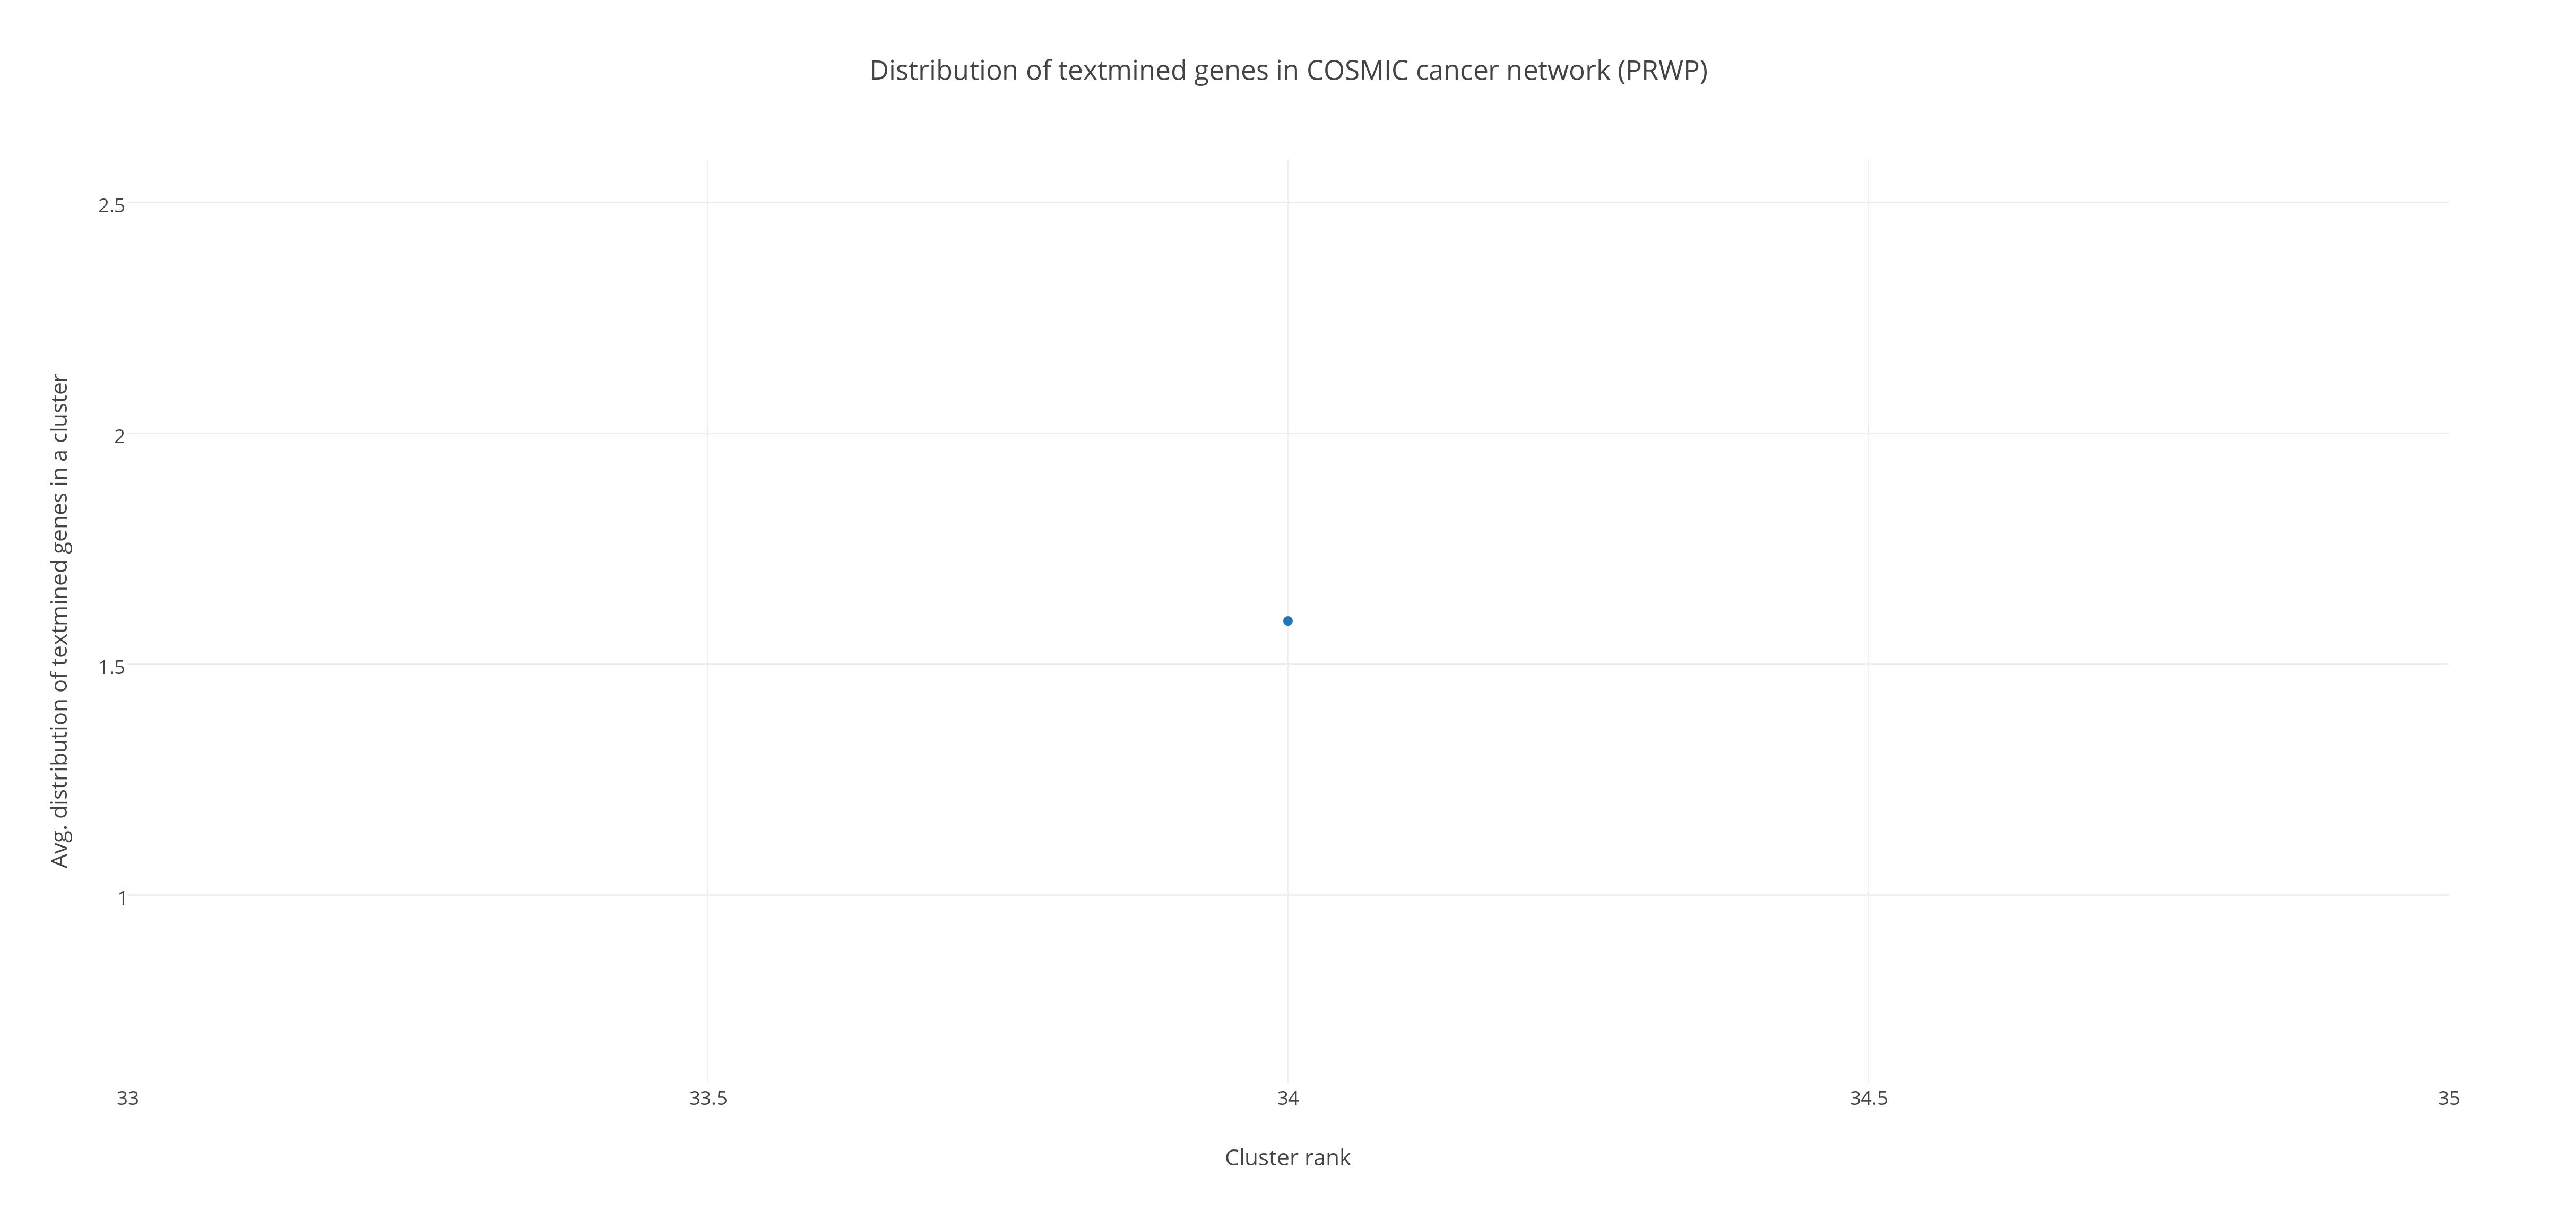
\includegraphics[width=15cm]{Distribution_of_textmined_genes_in_COSMIC_cancer_network_PRWP}
%\end{figure}
%\begin{figure}
%    \label{fig:txt-cosmic-maa}
%    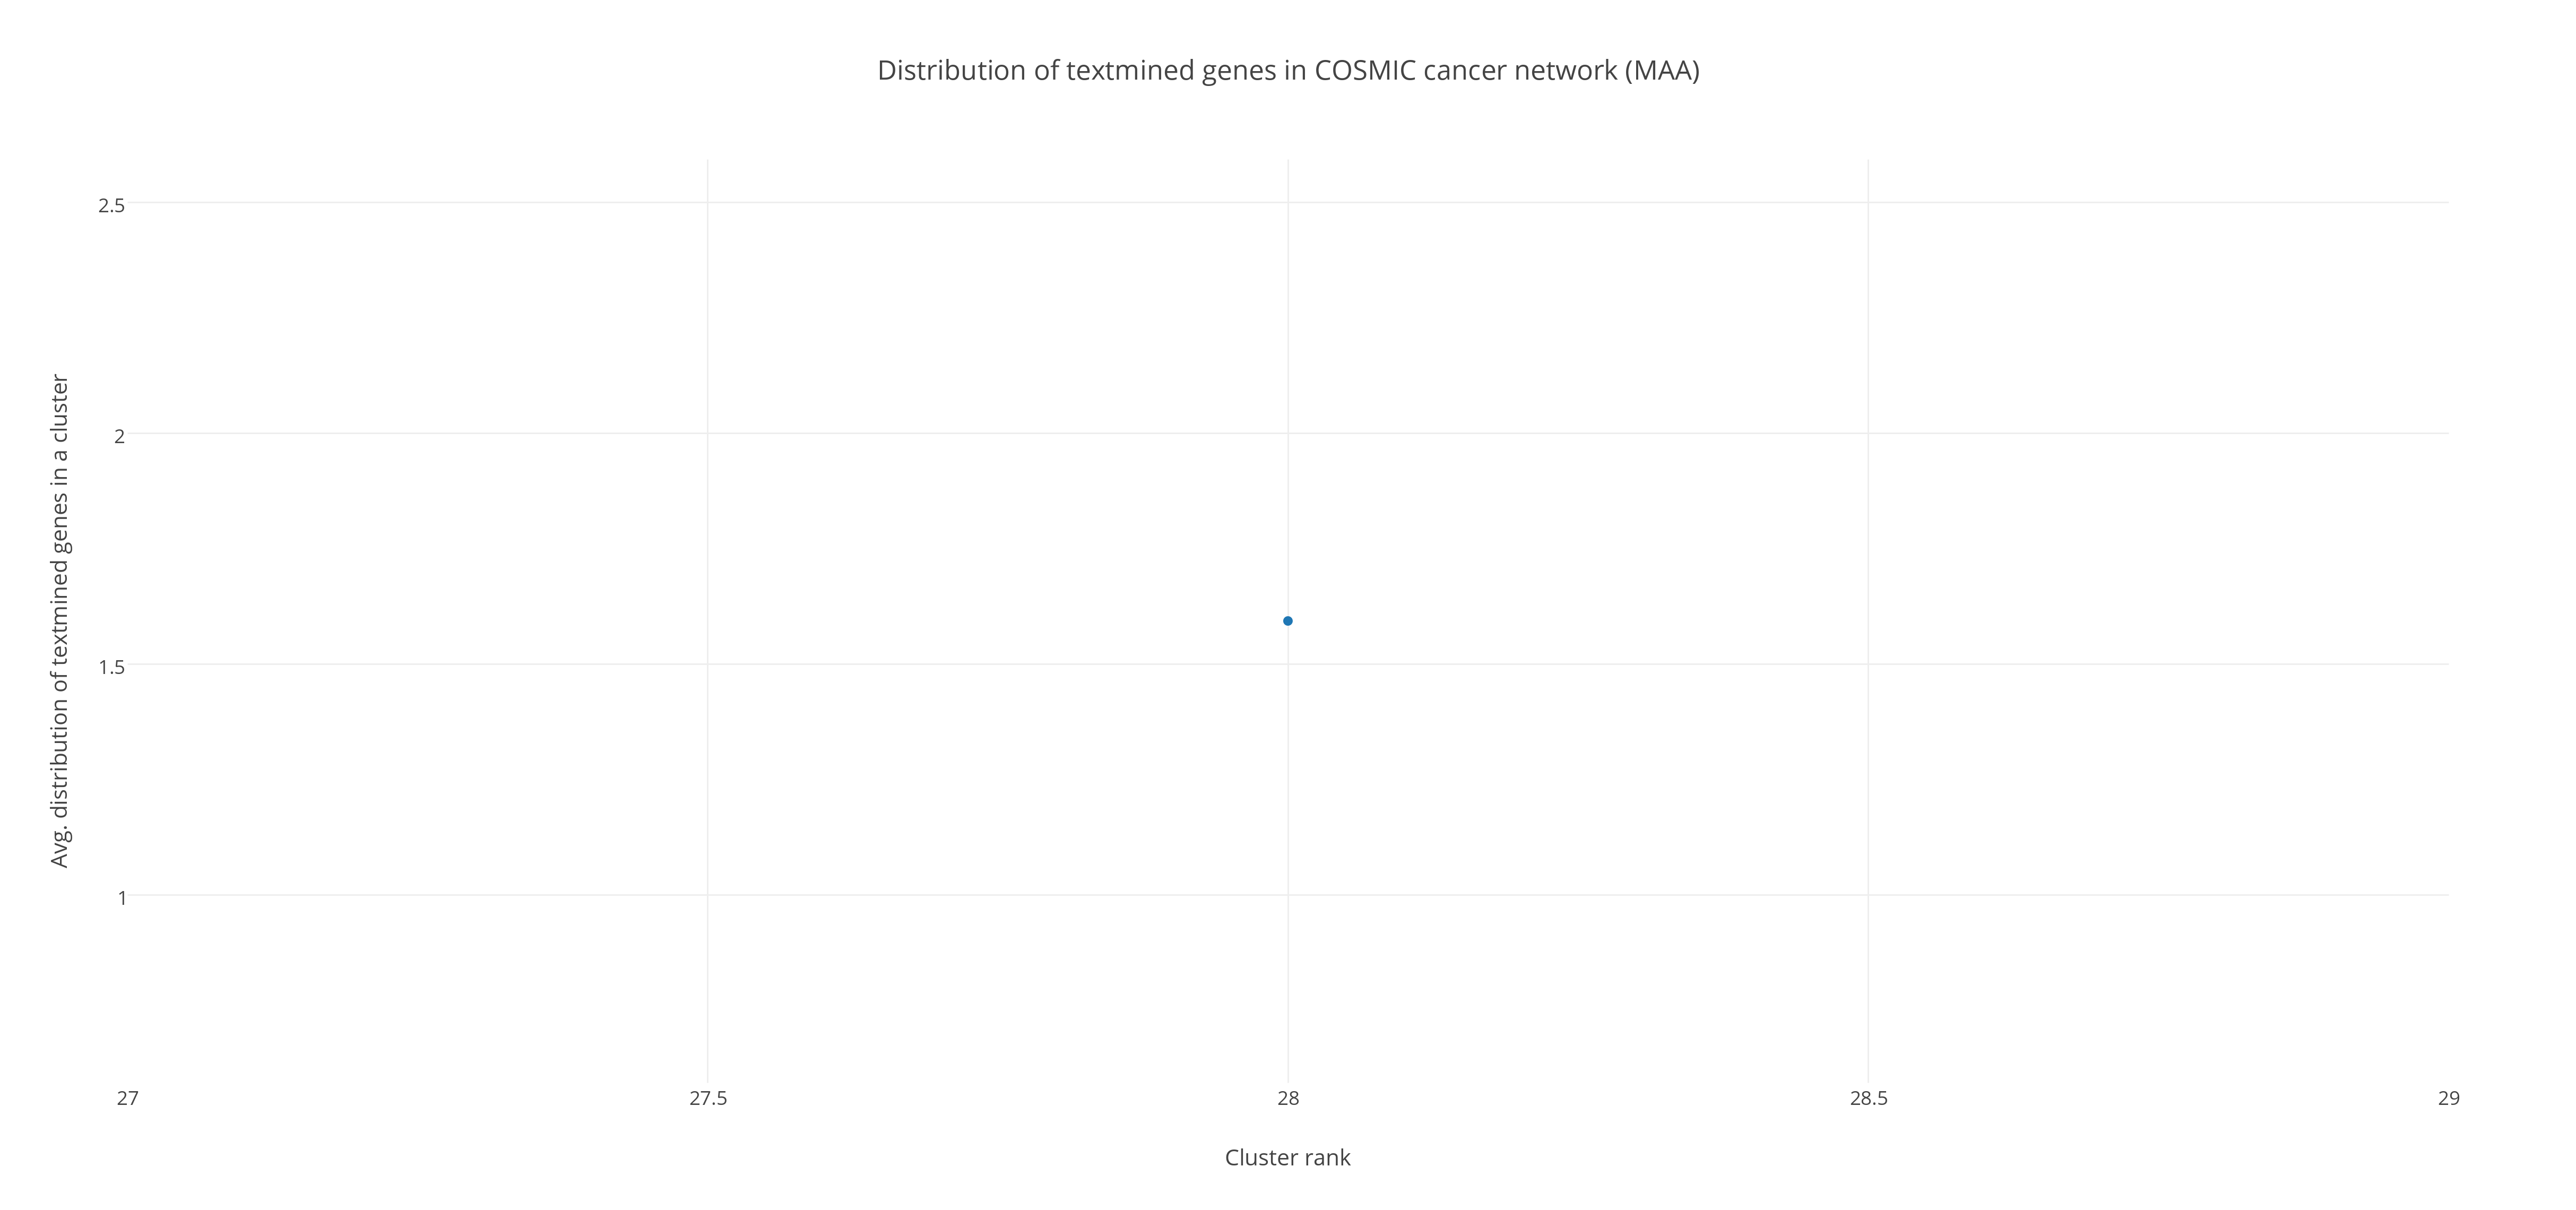
\includegraphics[width=15cm]{Distribution_of_textmined_genes_in_COSMIC_cancer_network_MAA}
%\end{figure}
%\begin{figure}
%    \label{fig:know-cosmic-prwp}
%    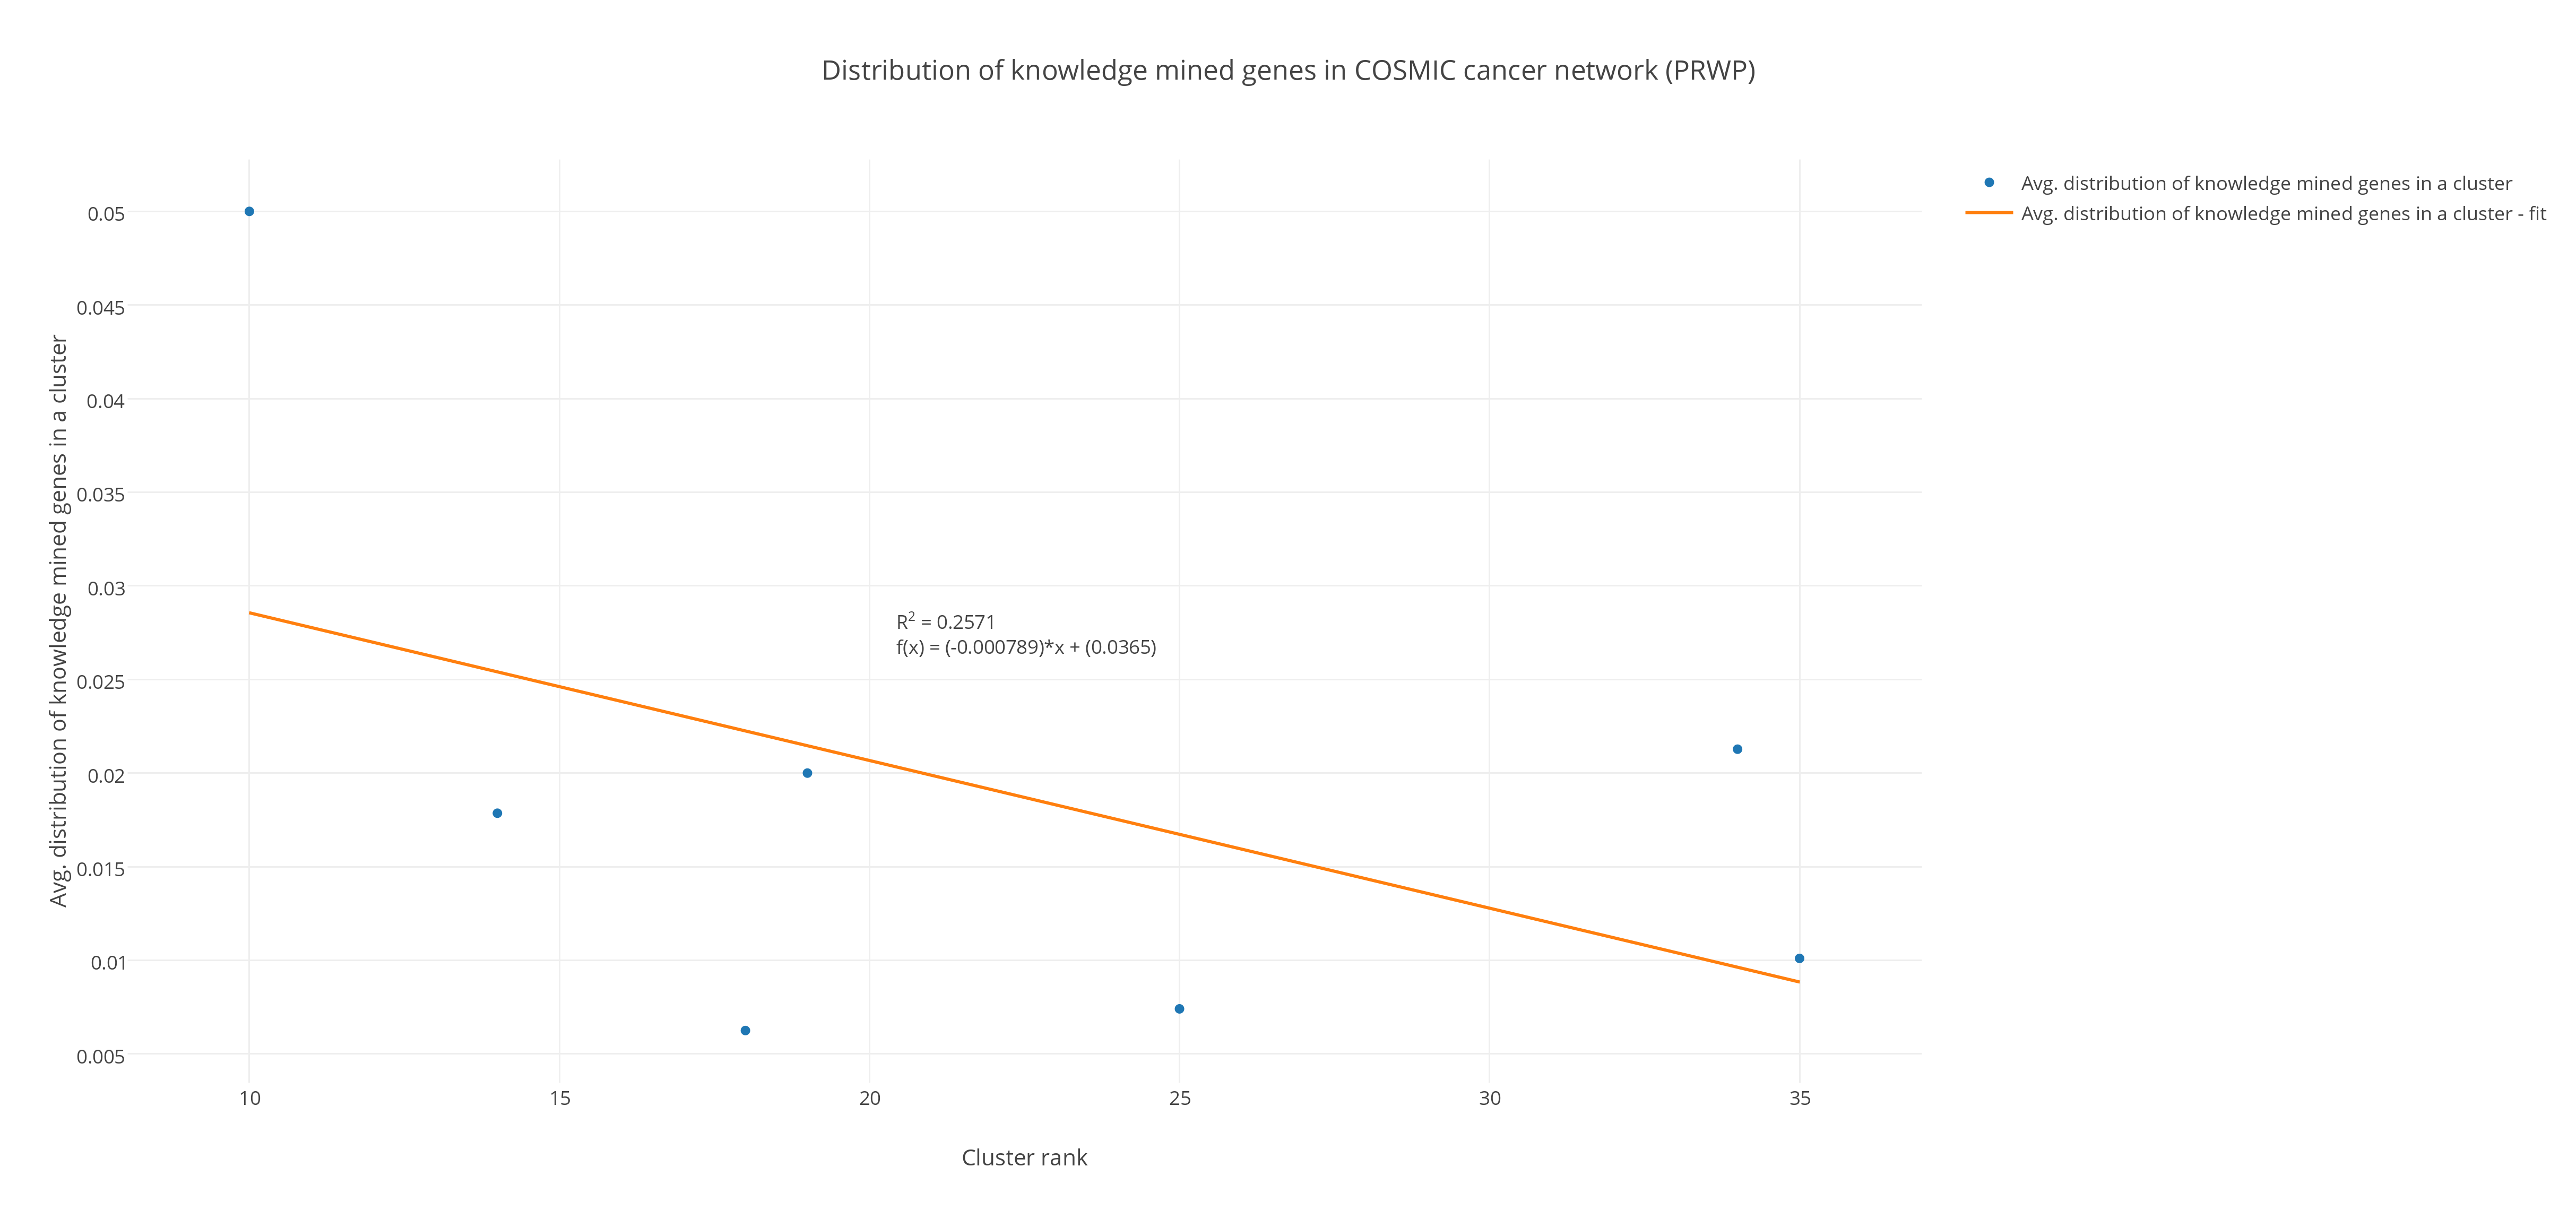
\includegraphics[width=15cm]{Distribution_of_knowledge_mined_genes_in_COSMIC_cancer_network_PRWP}
%\end{figure}
%\begin{figure}
%    \label{fig:know-cosmic-maa}
%    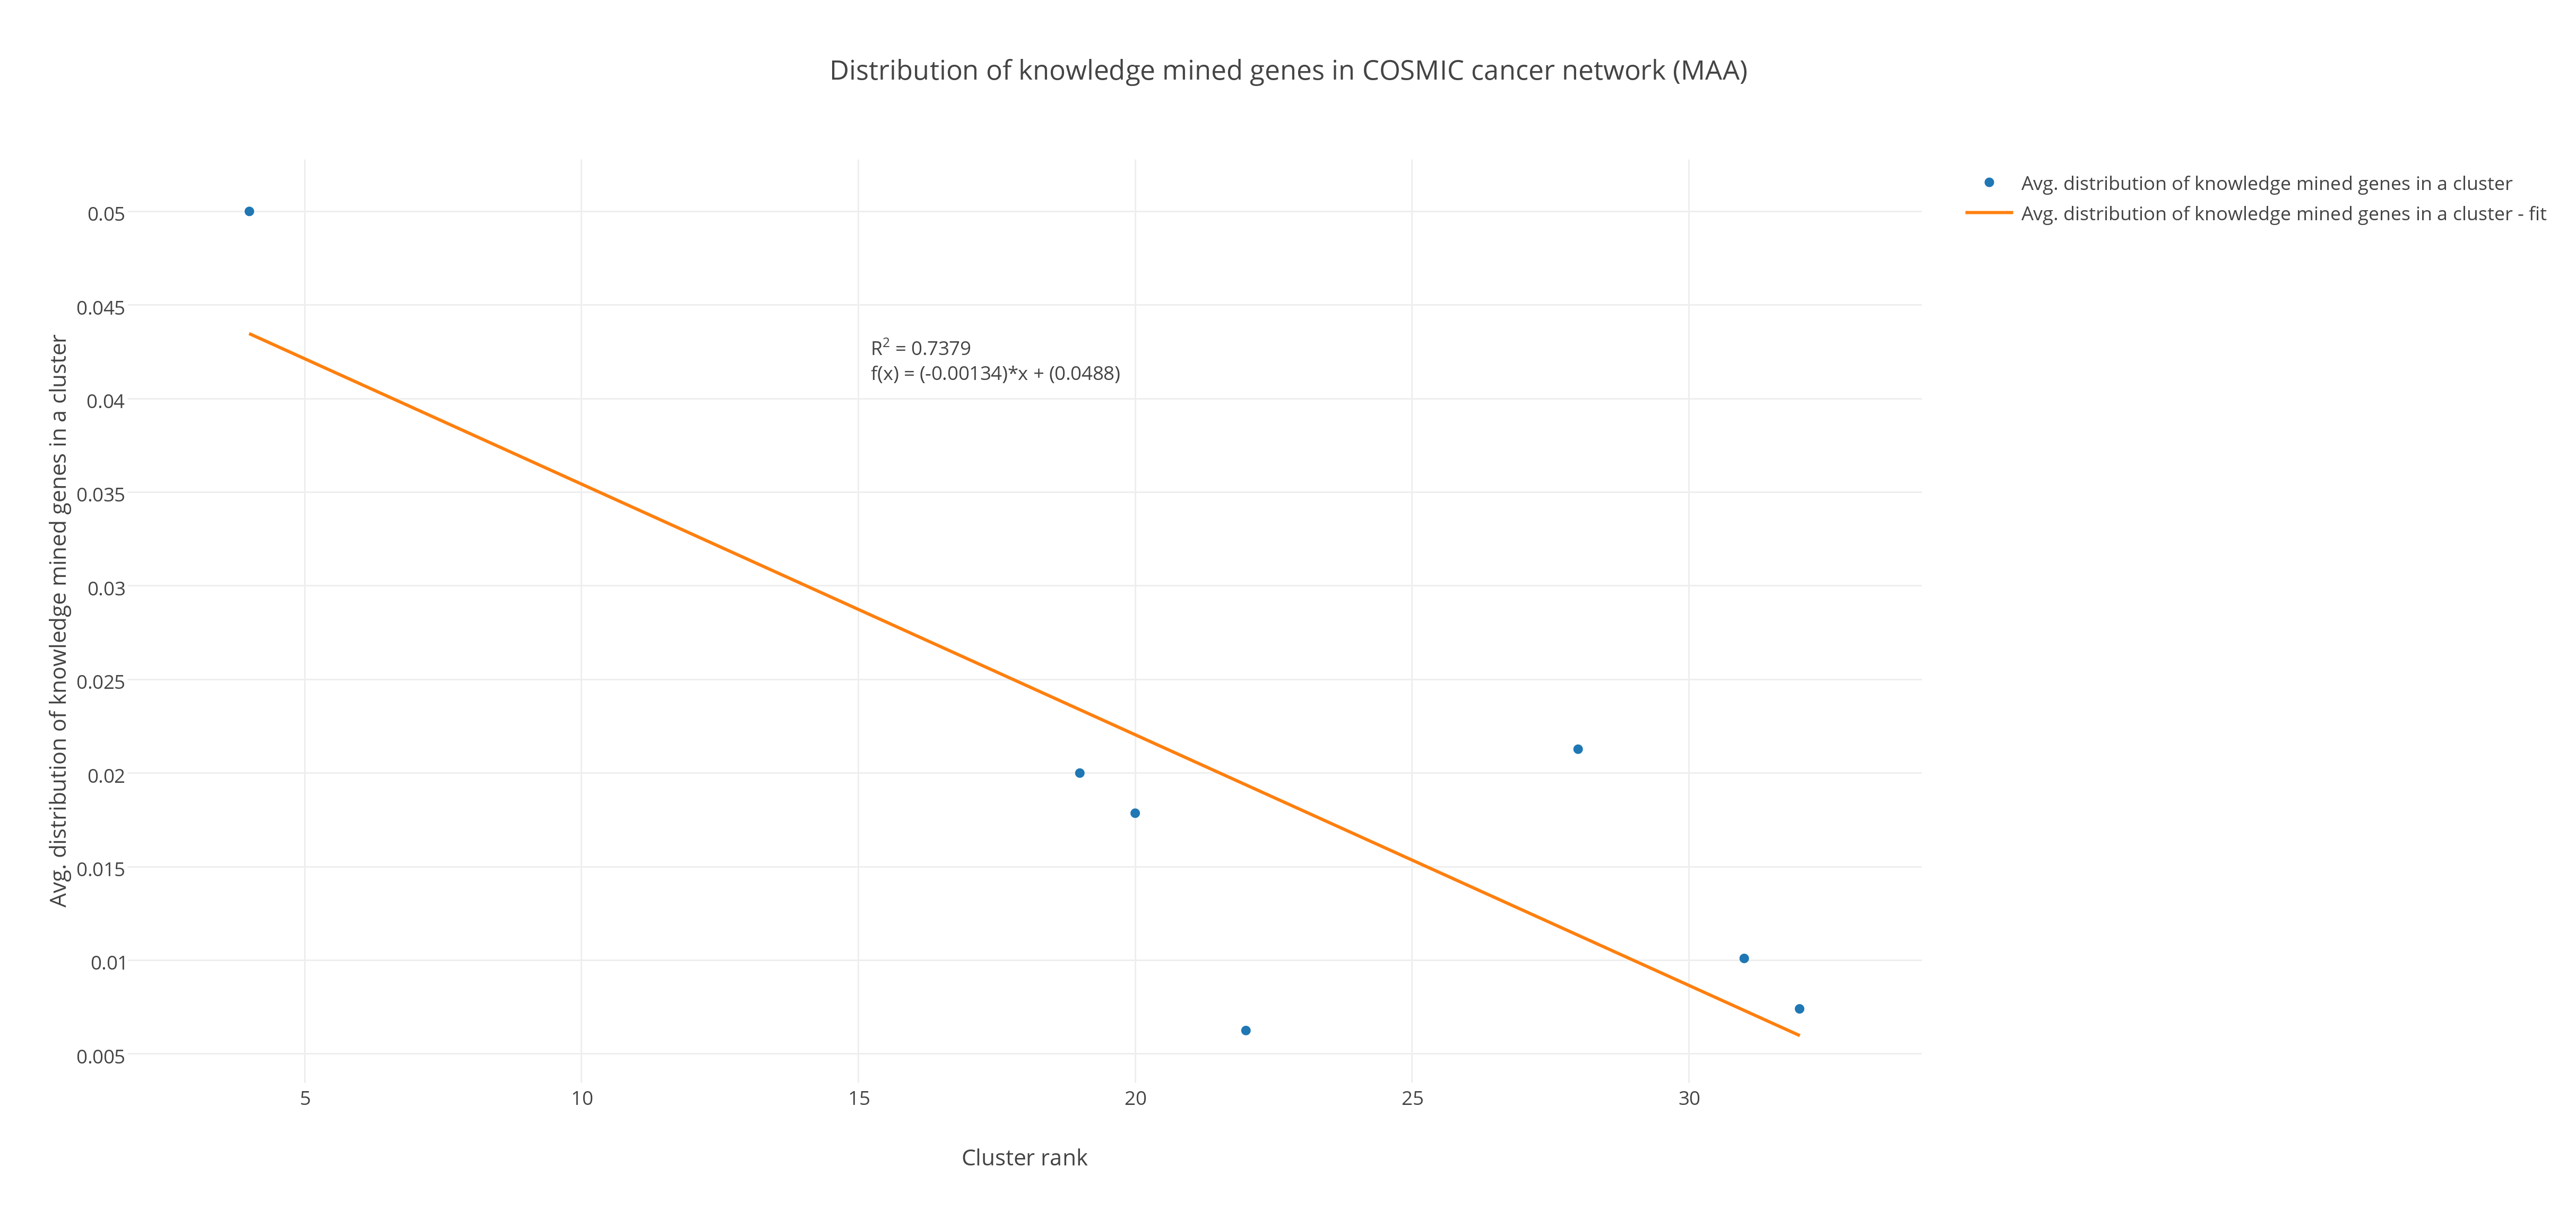
\includegraphics[width=15cm]{Distribution_of_knowledge_mined_genes_in_COSMIC_cancer_network_MAA}
%\end{figure}
%\begin{figure}
%    \label{fig:exp-cosmic-prwp}
%    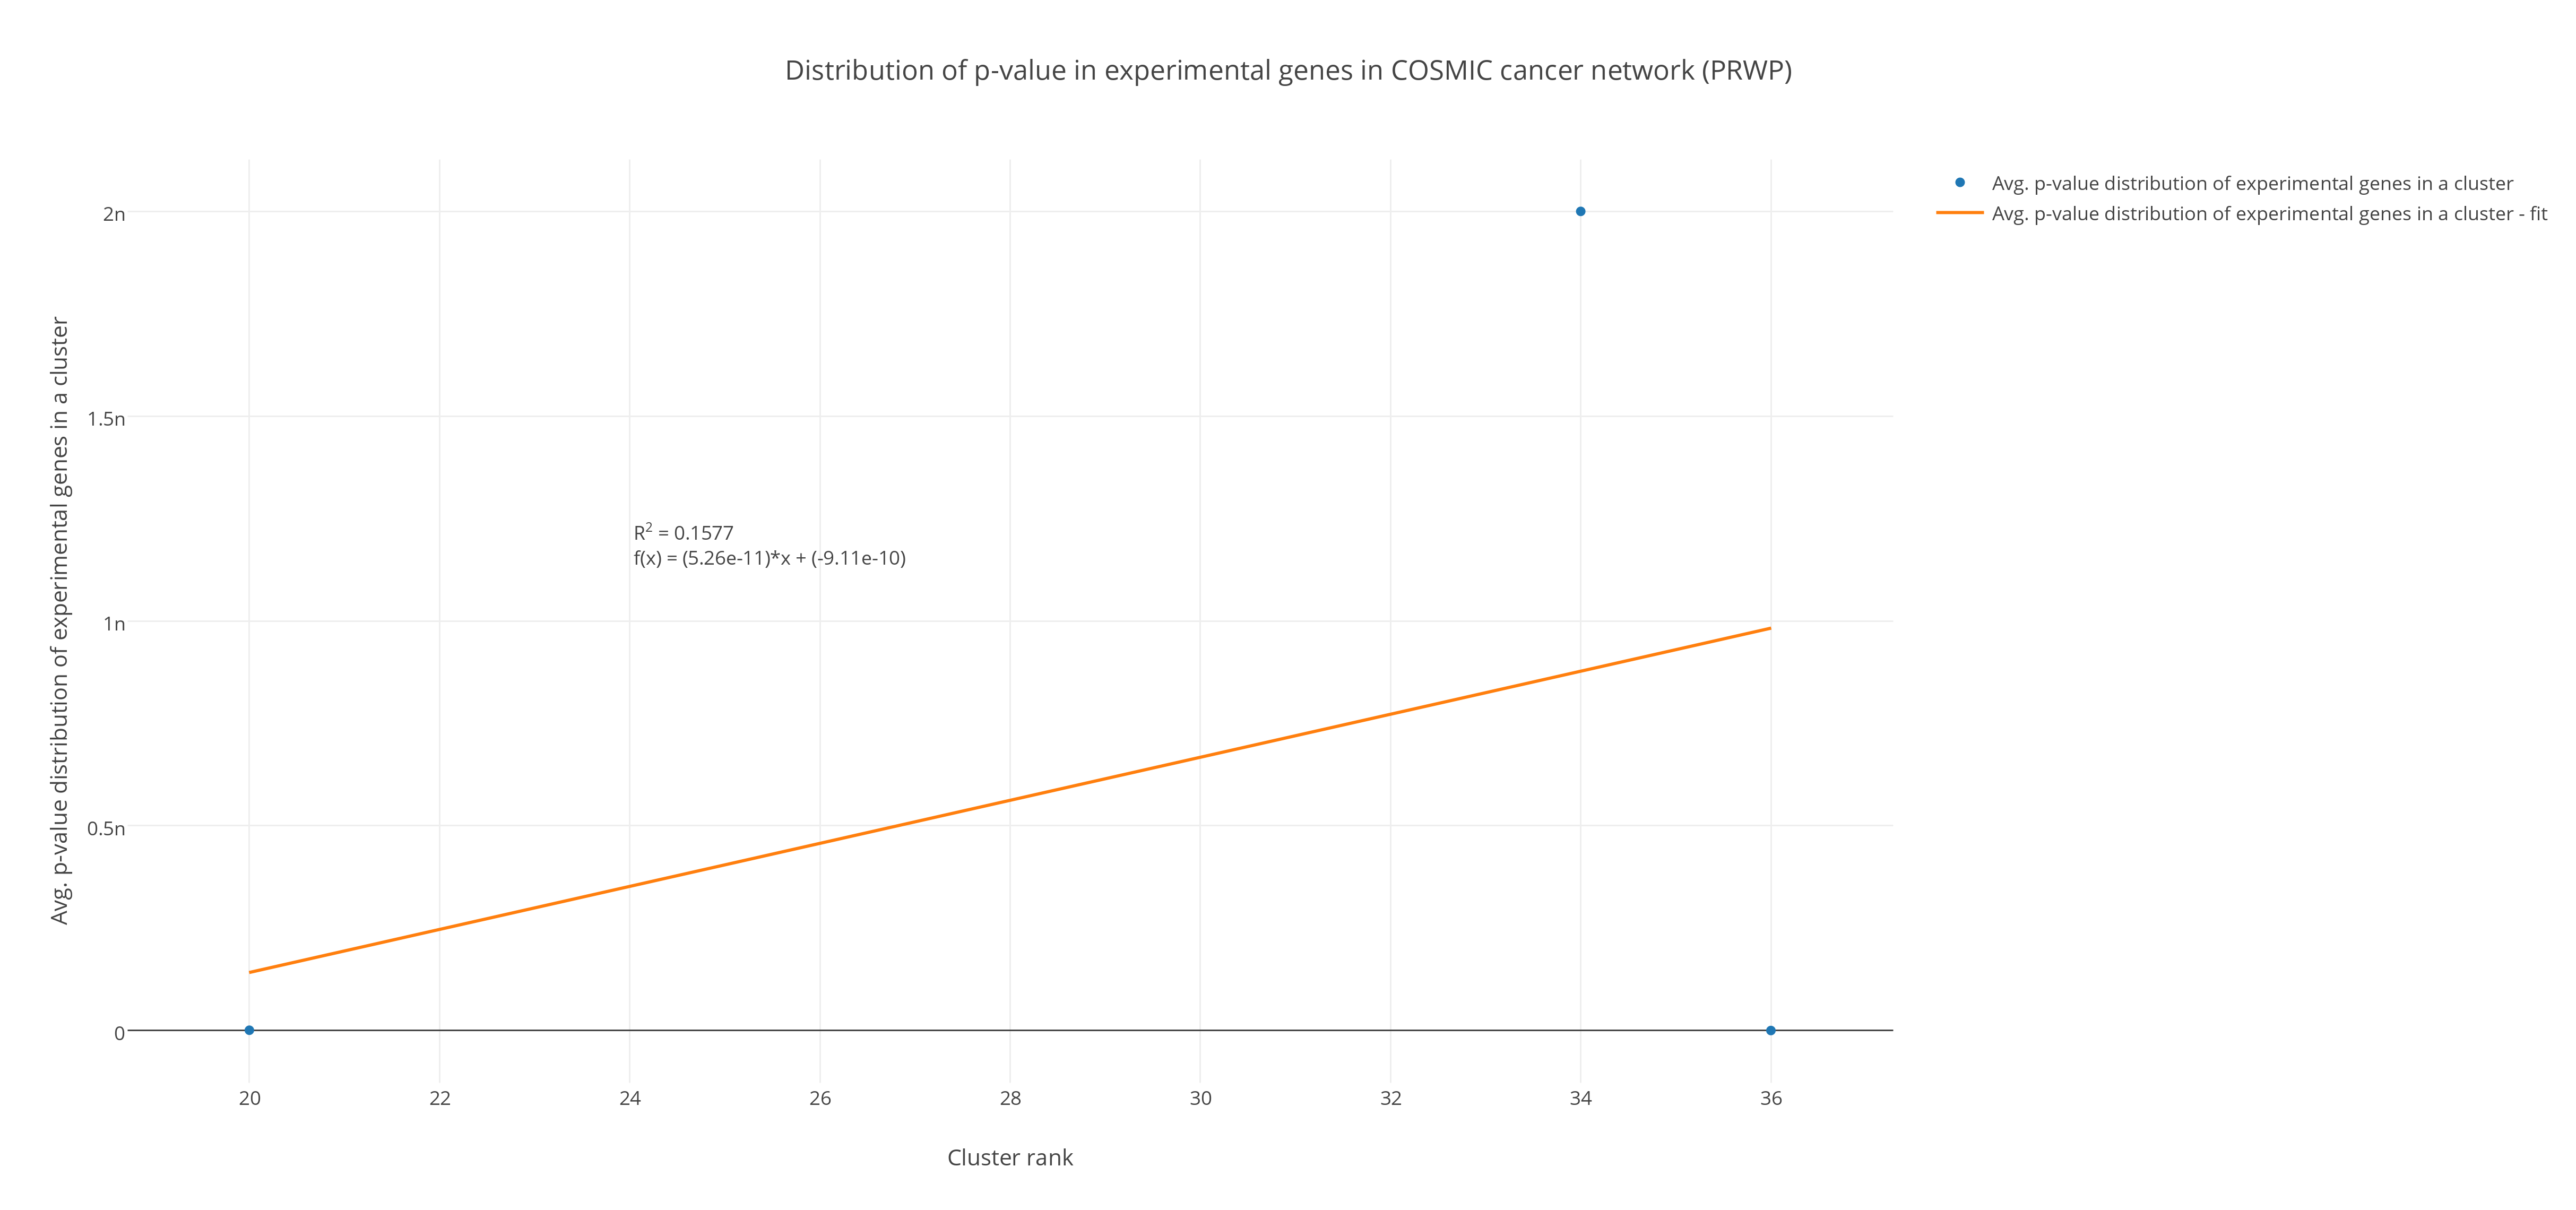
\includegraphics[width=15cm]{Distribution_of_p-value_in_experimental_genes_in_COSMIC_cancer_network_PRWP}
%\end{figure}
%\begin{figure}
%    \label{fig:exp-cosmic-maa}
%    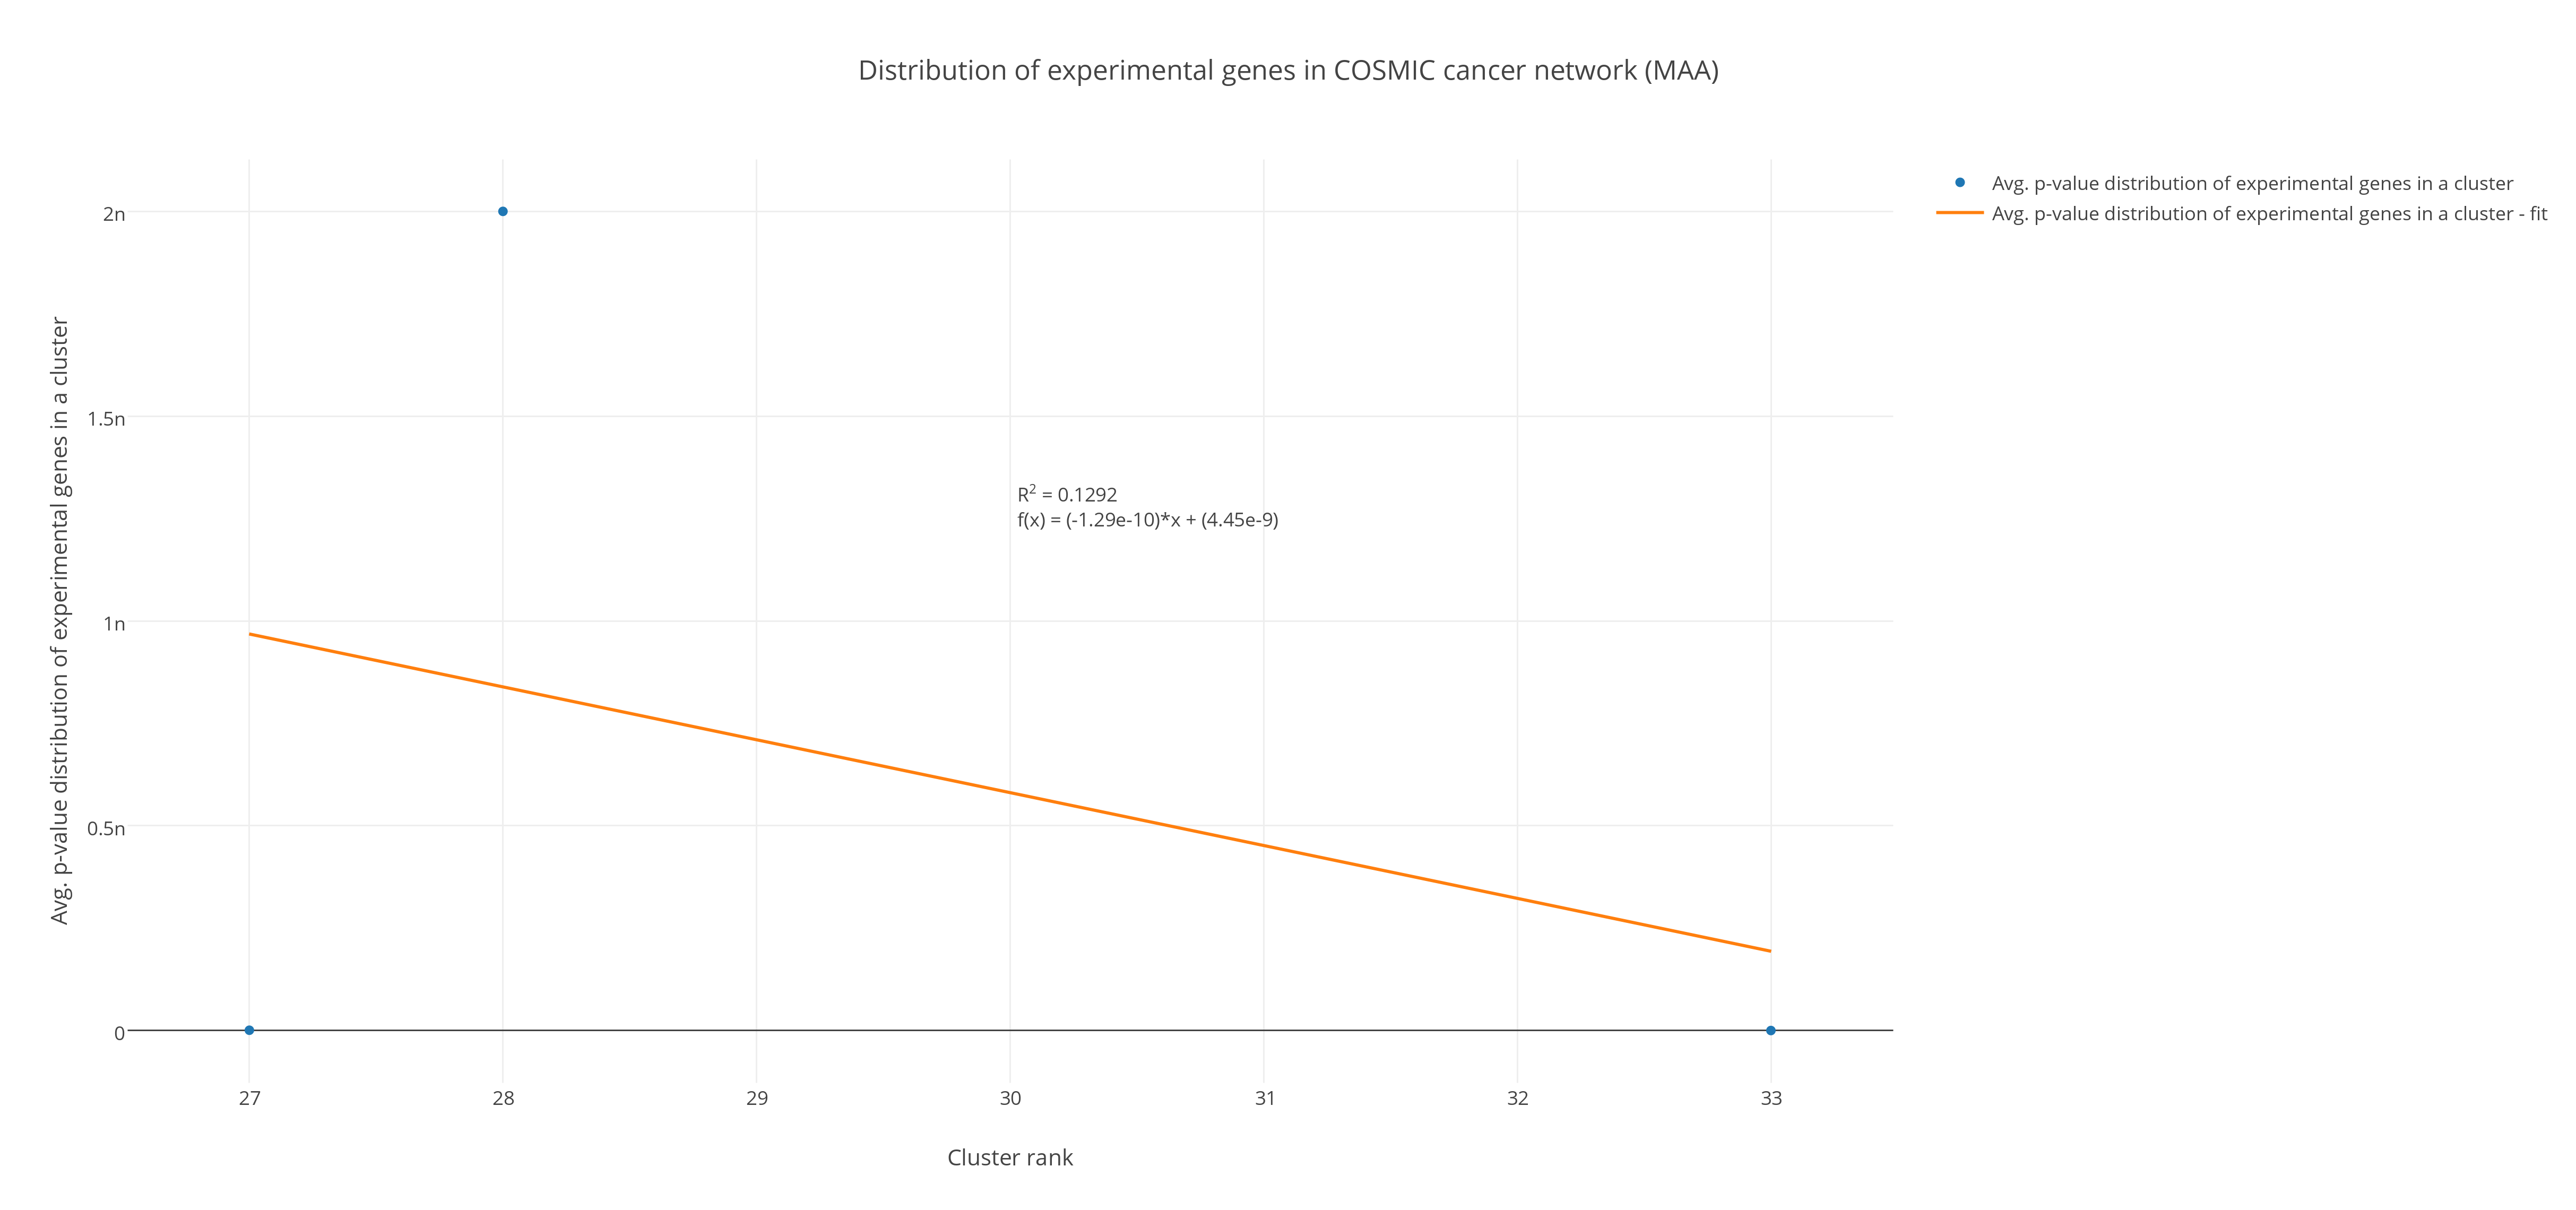
\includegraphics[width=15cm]{Distribution_of_experimental_genes_in_COSMIC_cancer_network_MAA}
%\end{figure}

% new figures
% prwp
\begin{figure}
    \label{fig:txt-iref-prwp}
    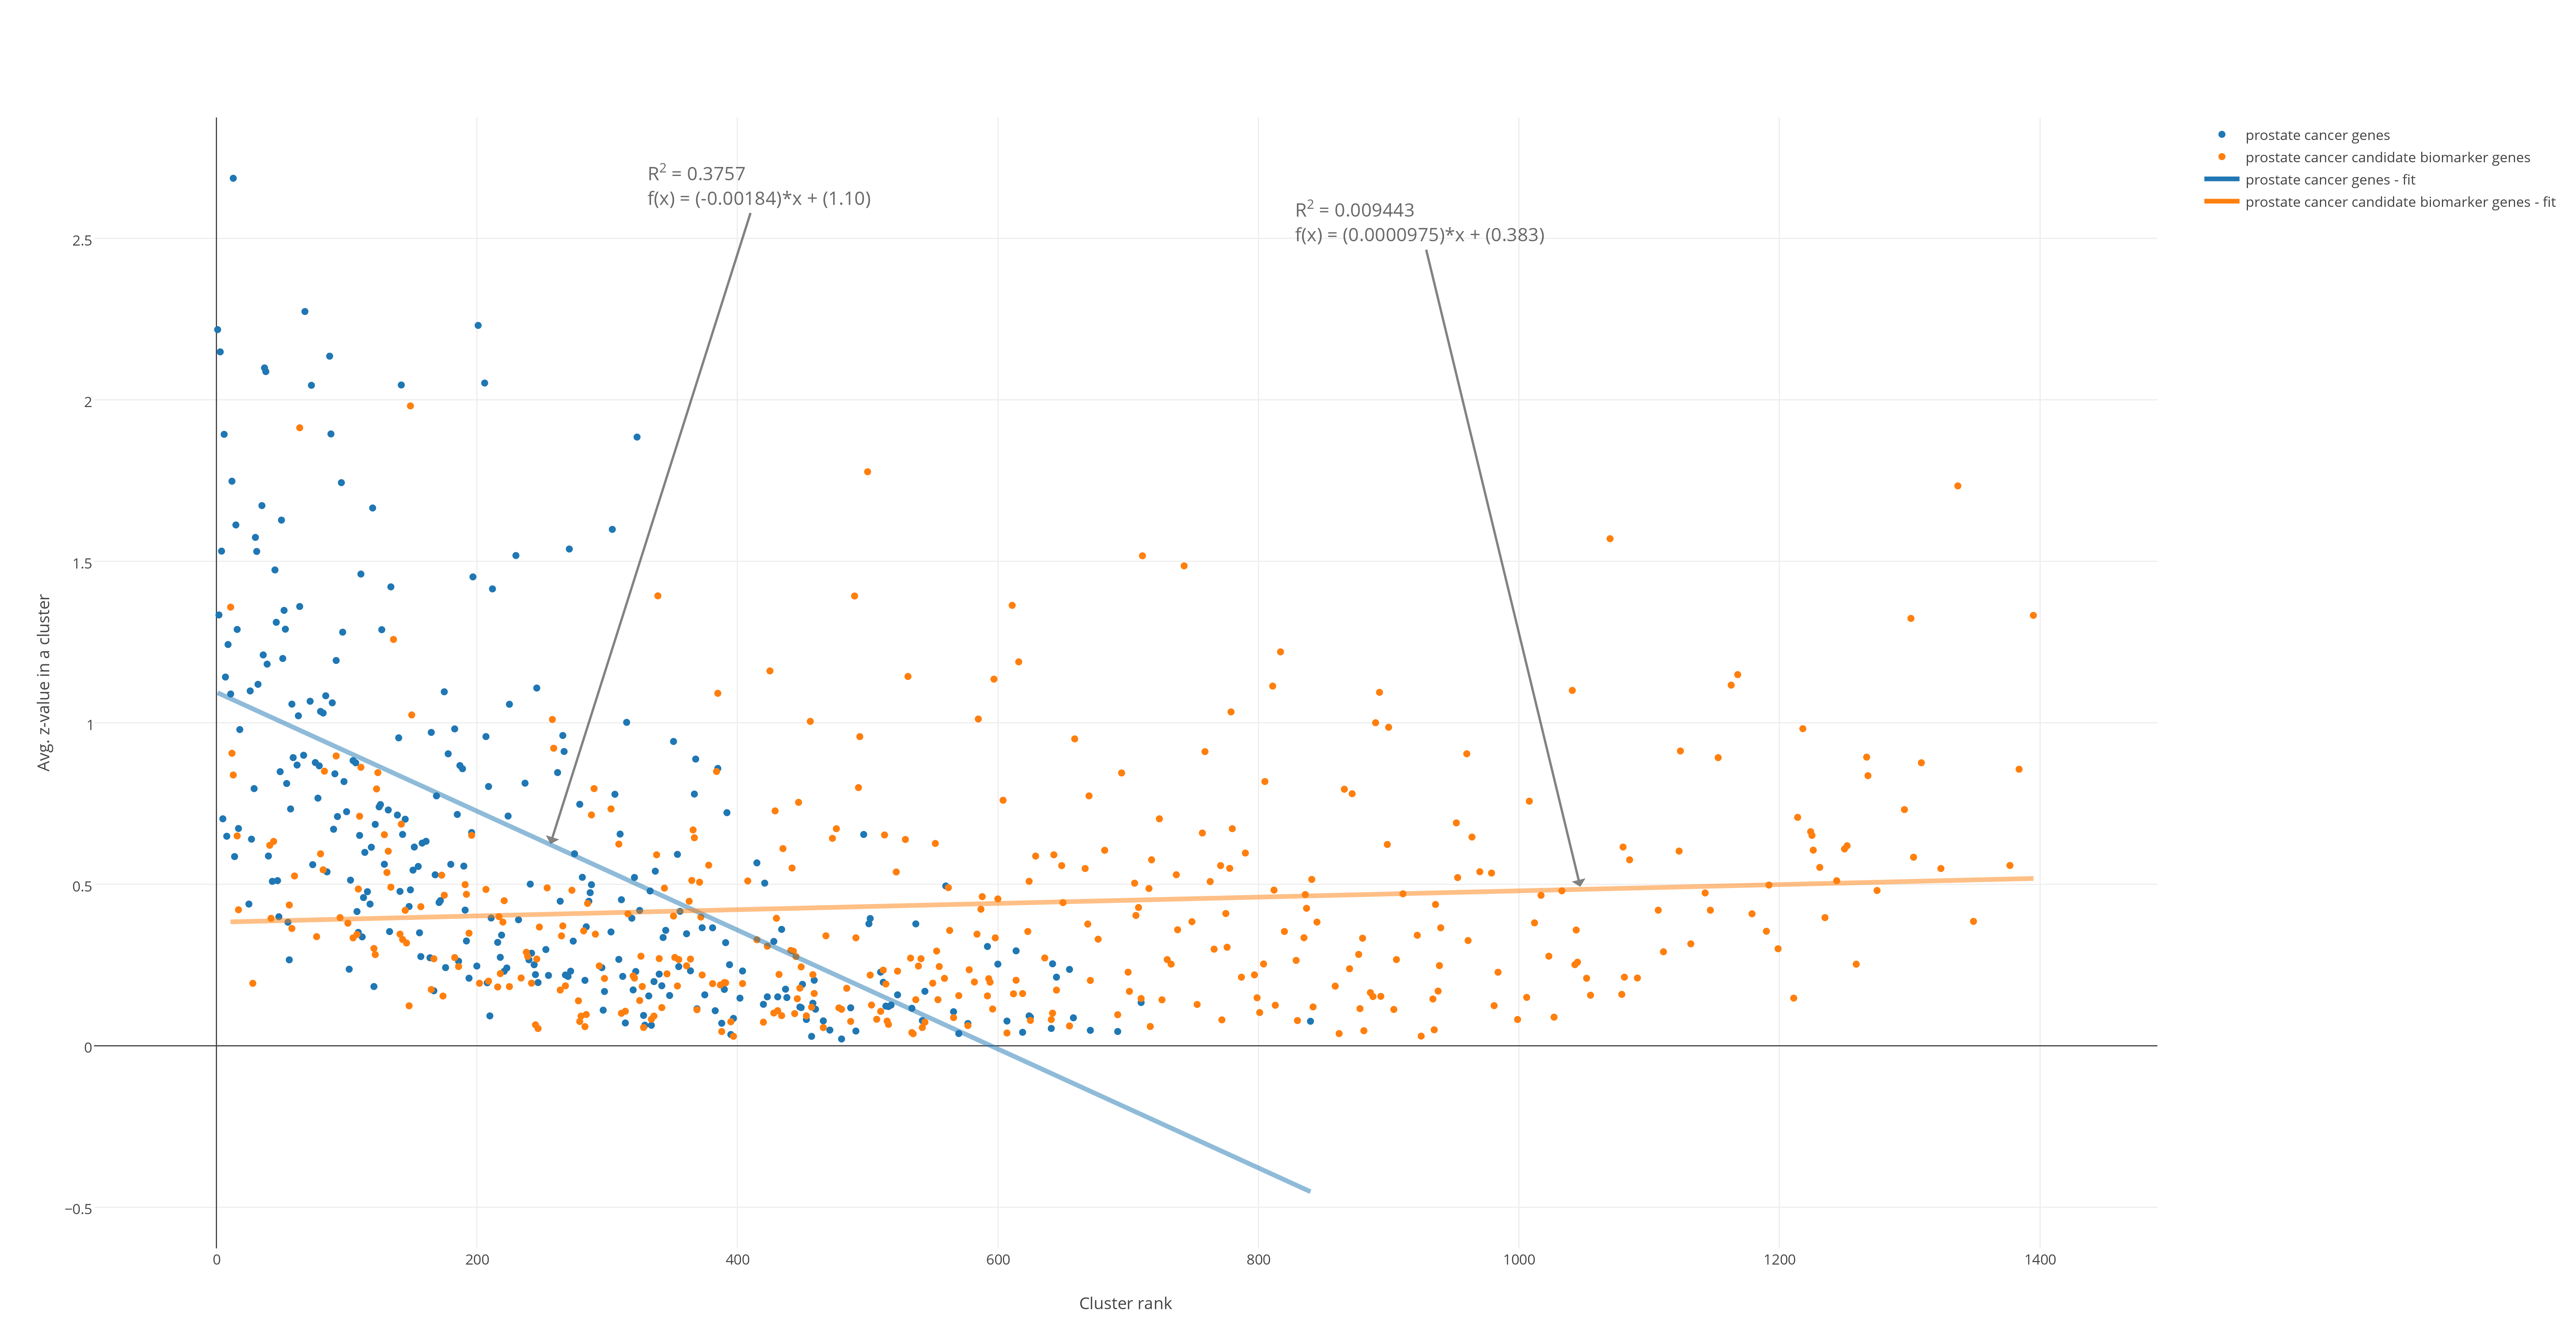
\includegraphics[width=15cm]{prwp_textmined_split}
\end{figure}
\begin{figure}
    \label{fig:know-iref-prwp}
    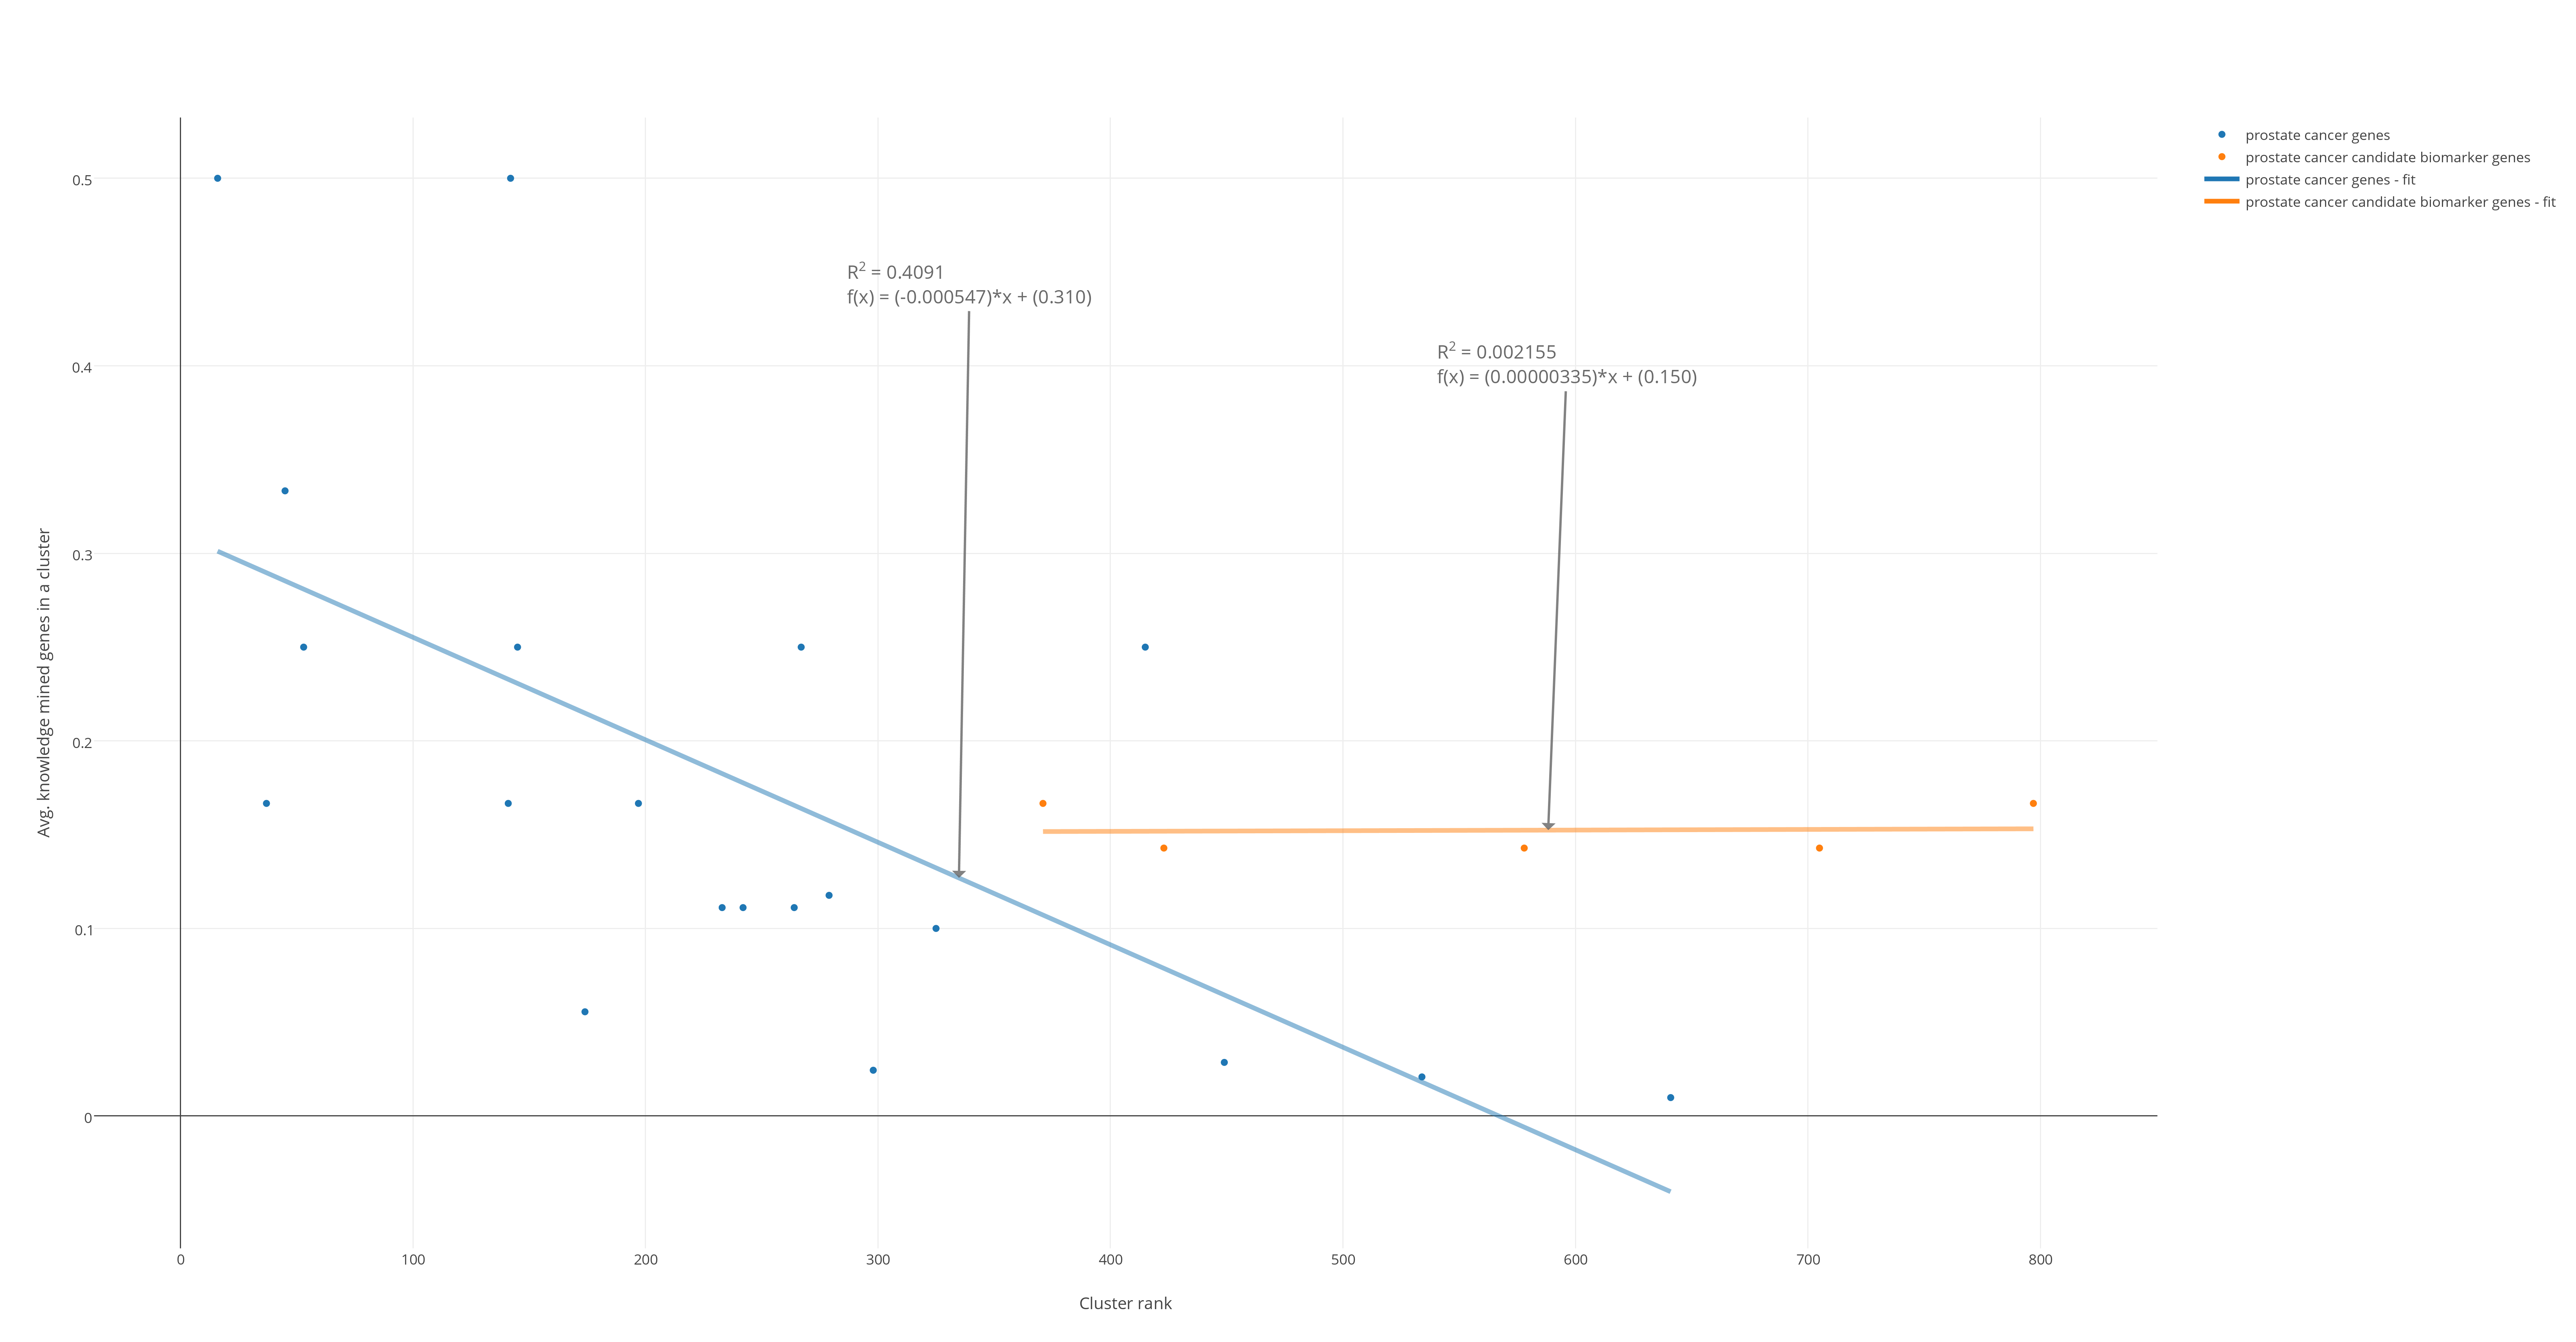
\includegraphics[width=15cm]{prwp_knowledge_split}
\end{figure}
\begin{figure}
    \label{fig:exp-iref-prwp}
    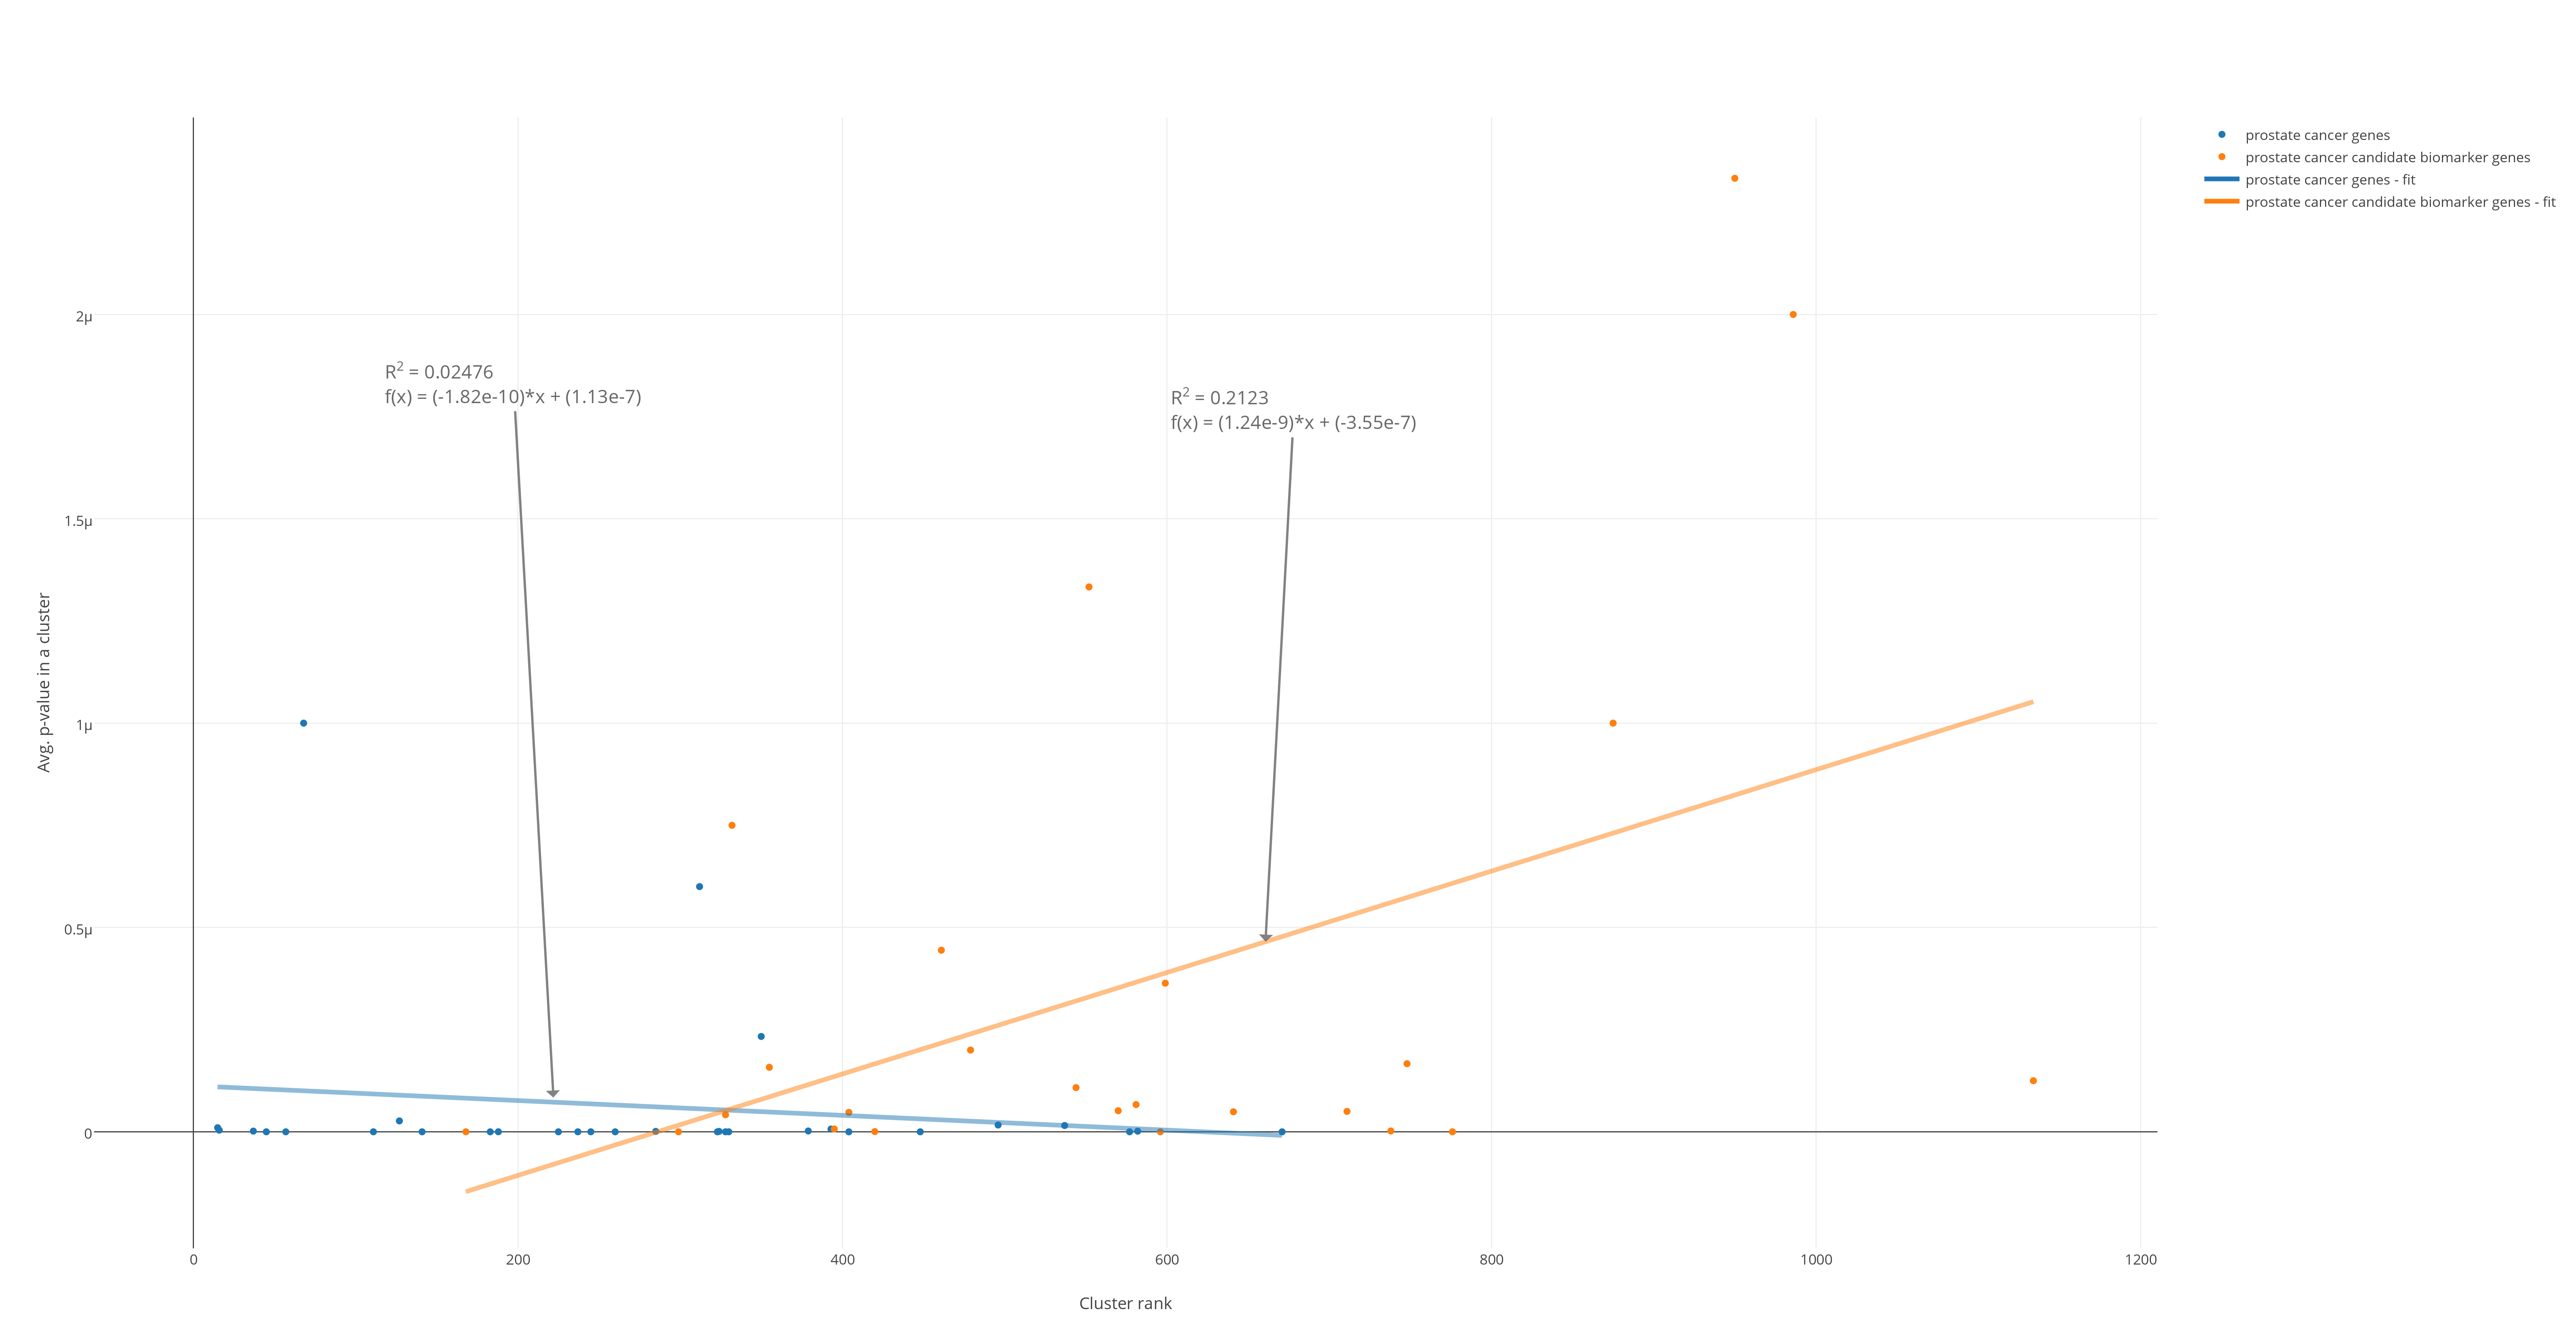
\includegraphics[width=15cm]{prwp_experimental_split}
\end{figure}
\begin{figure}
    \label{fig:txt-cosmic-prwp}
    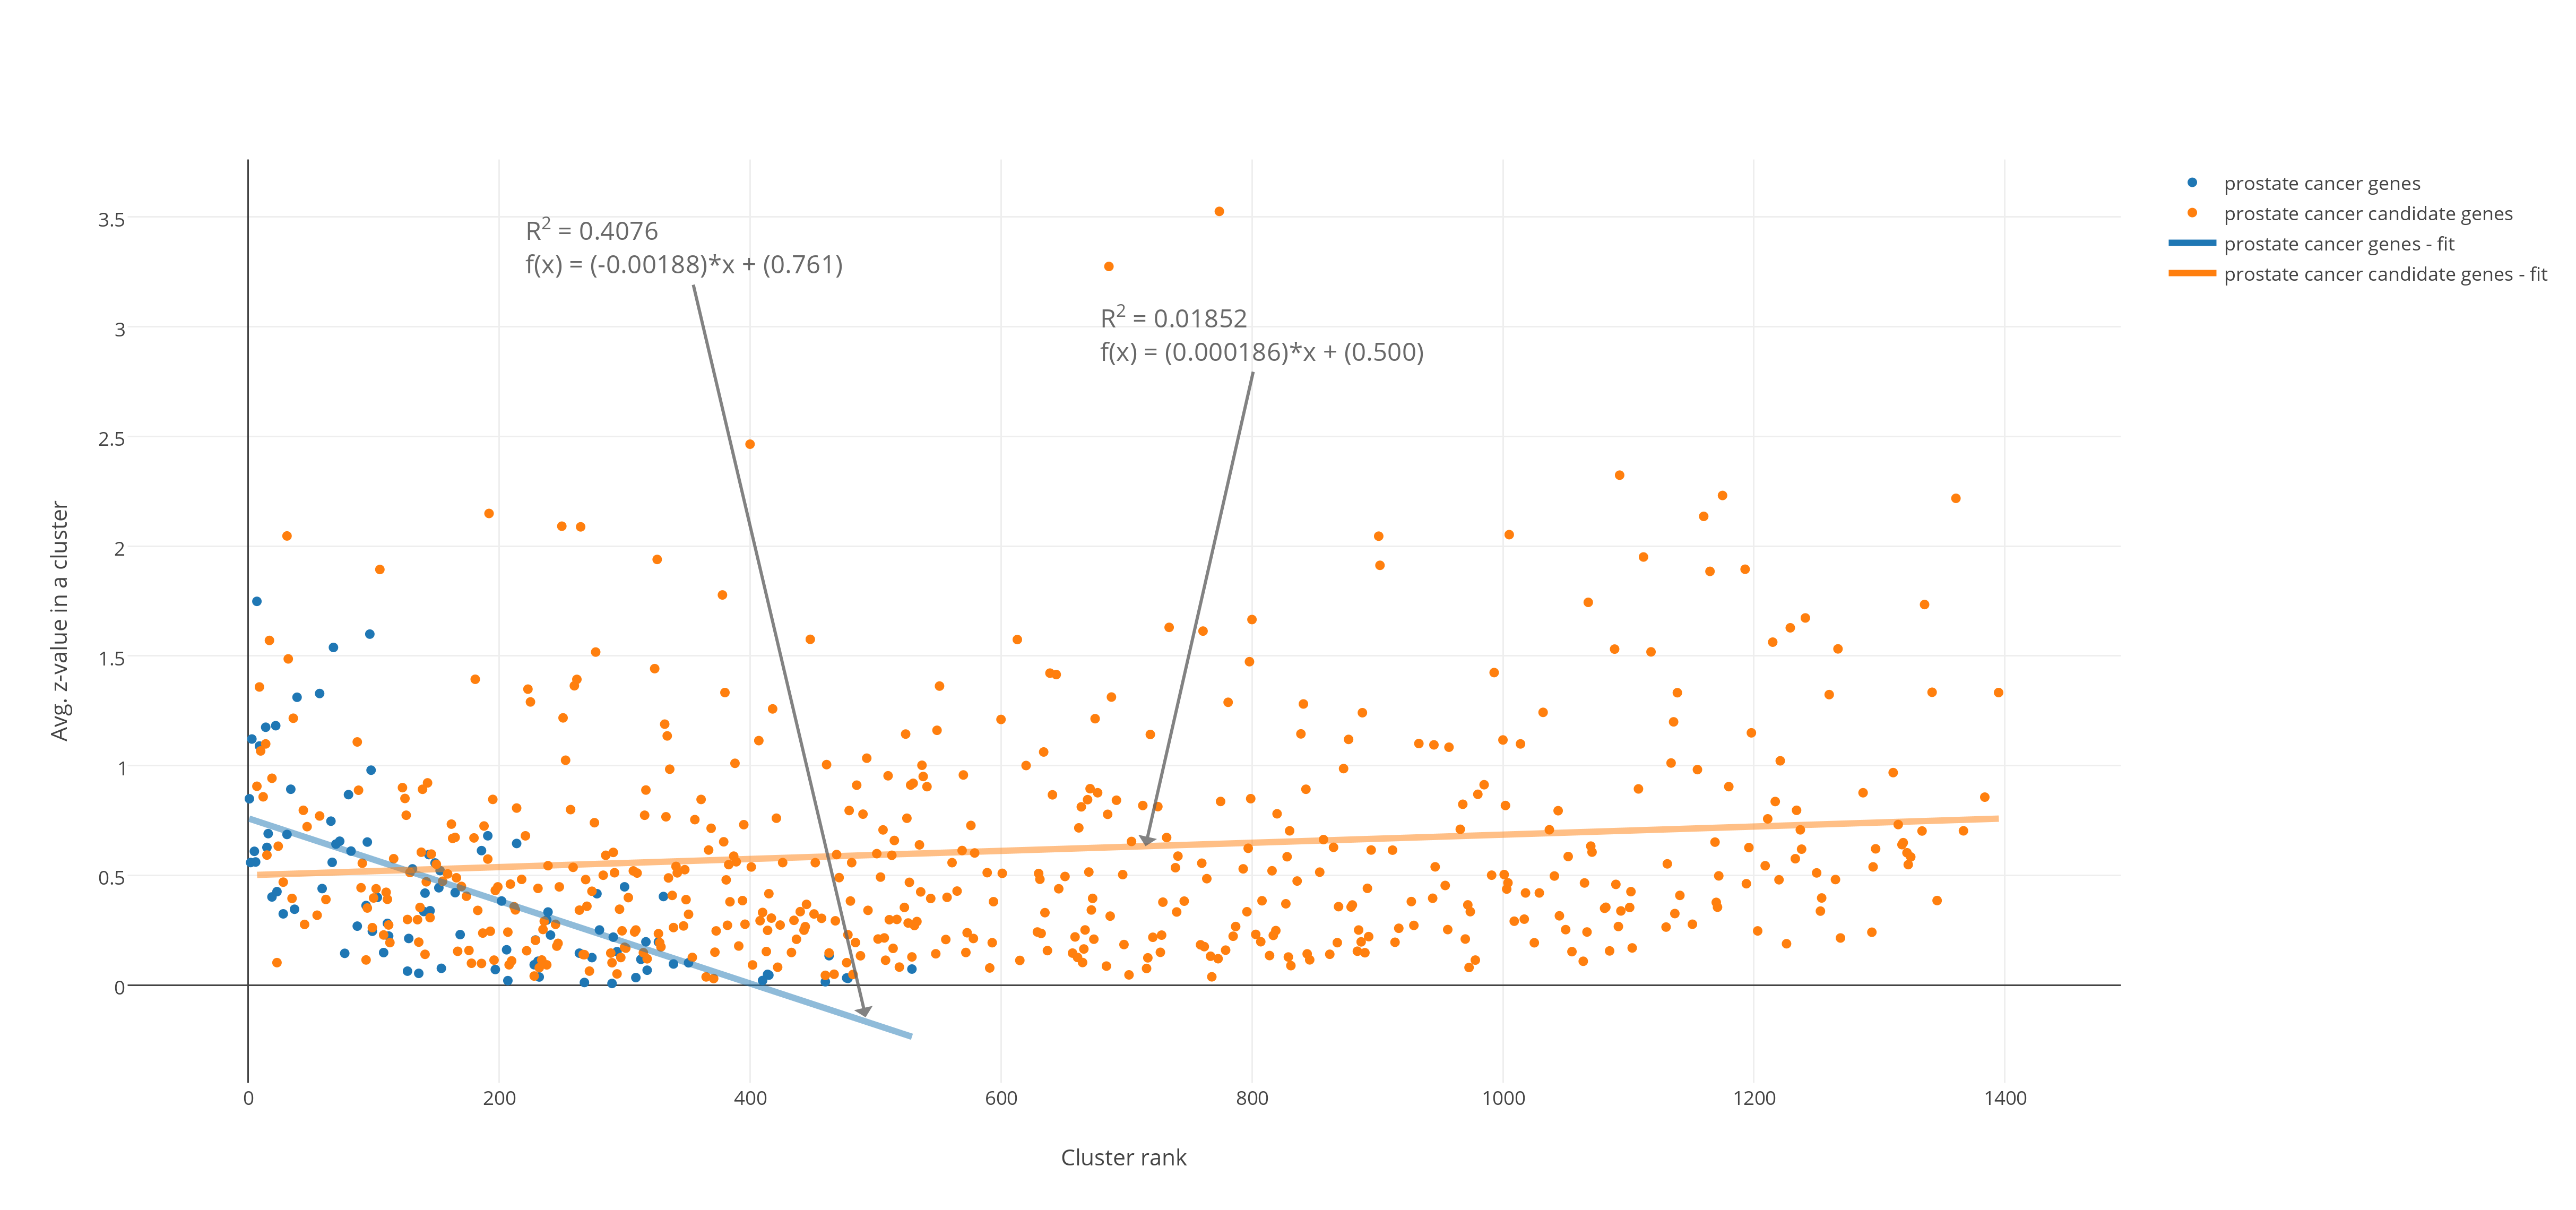
\includegraphics[width=15cm]{prwp_txt_split_cosmic}
\end{figure}
\begin{figure}
    \label{fig:know-cosmic-prwp}
    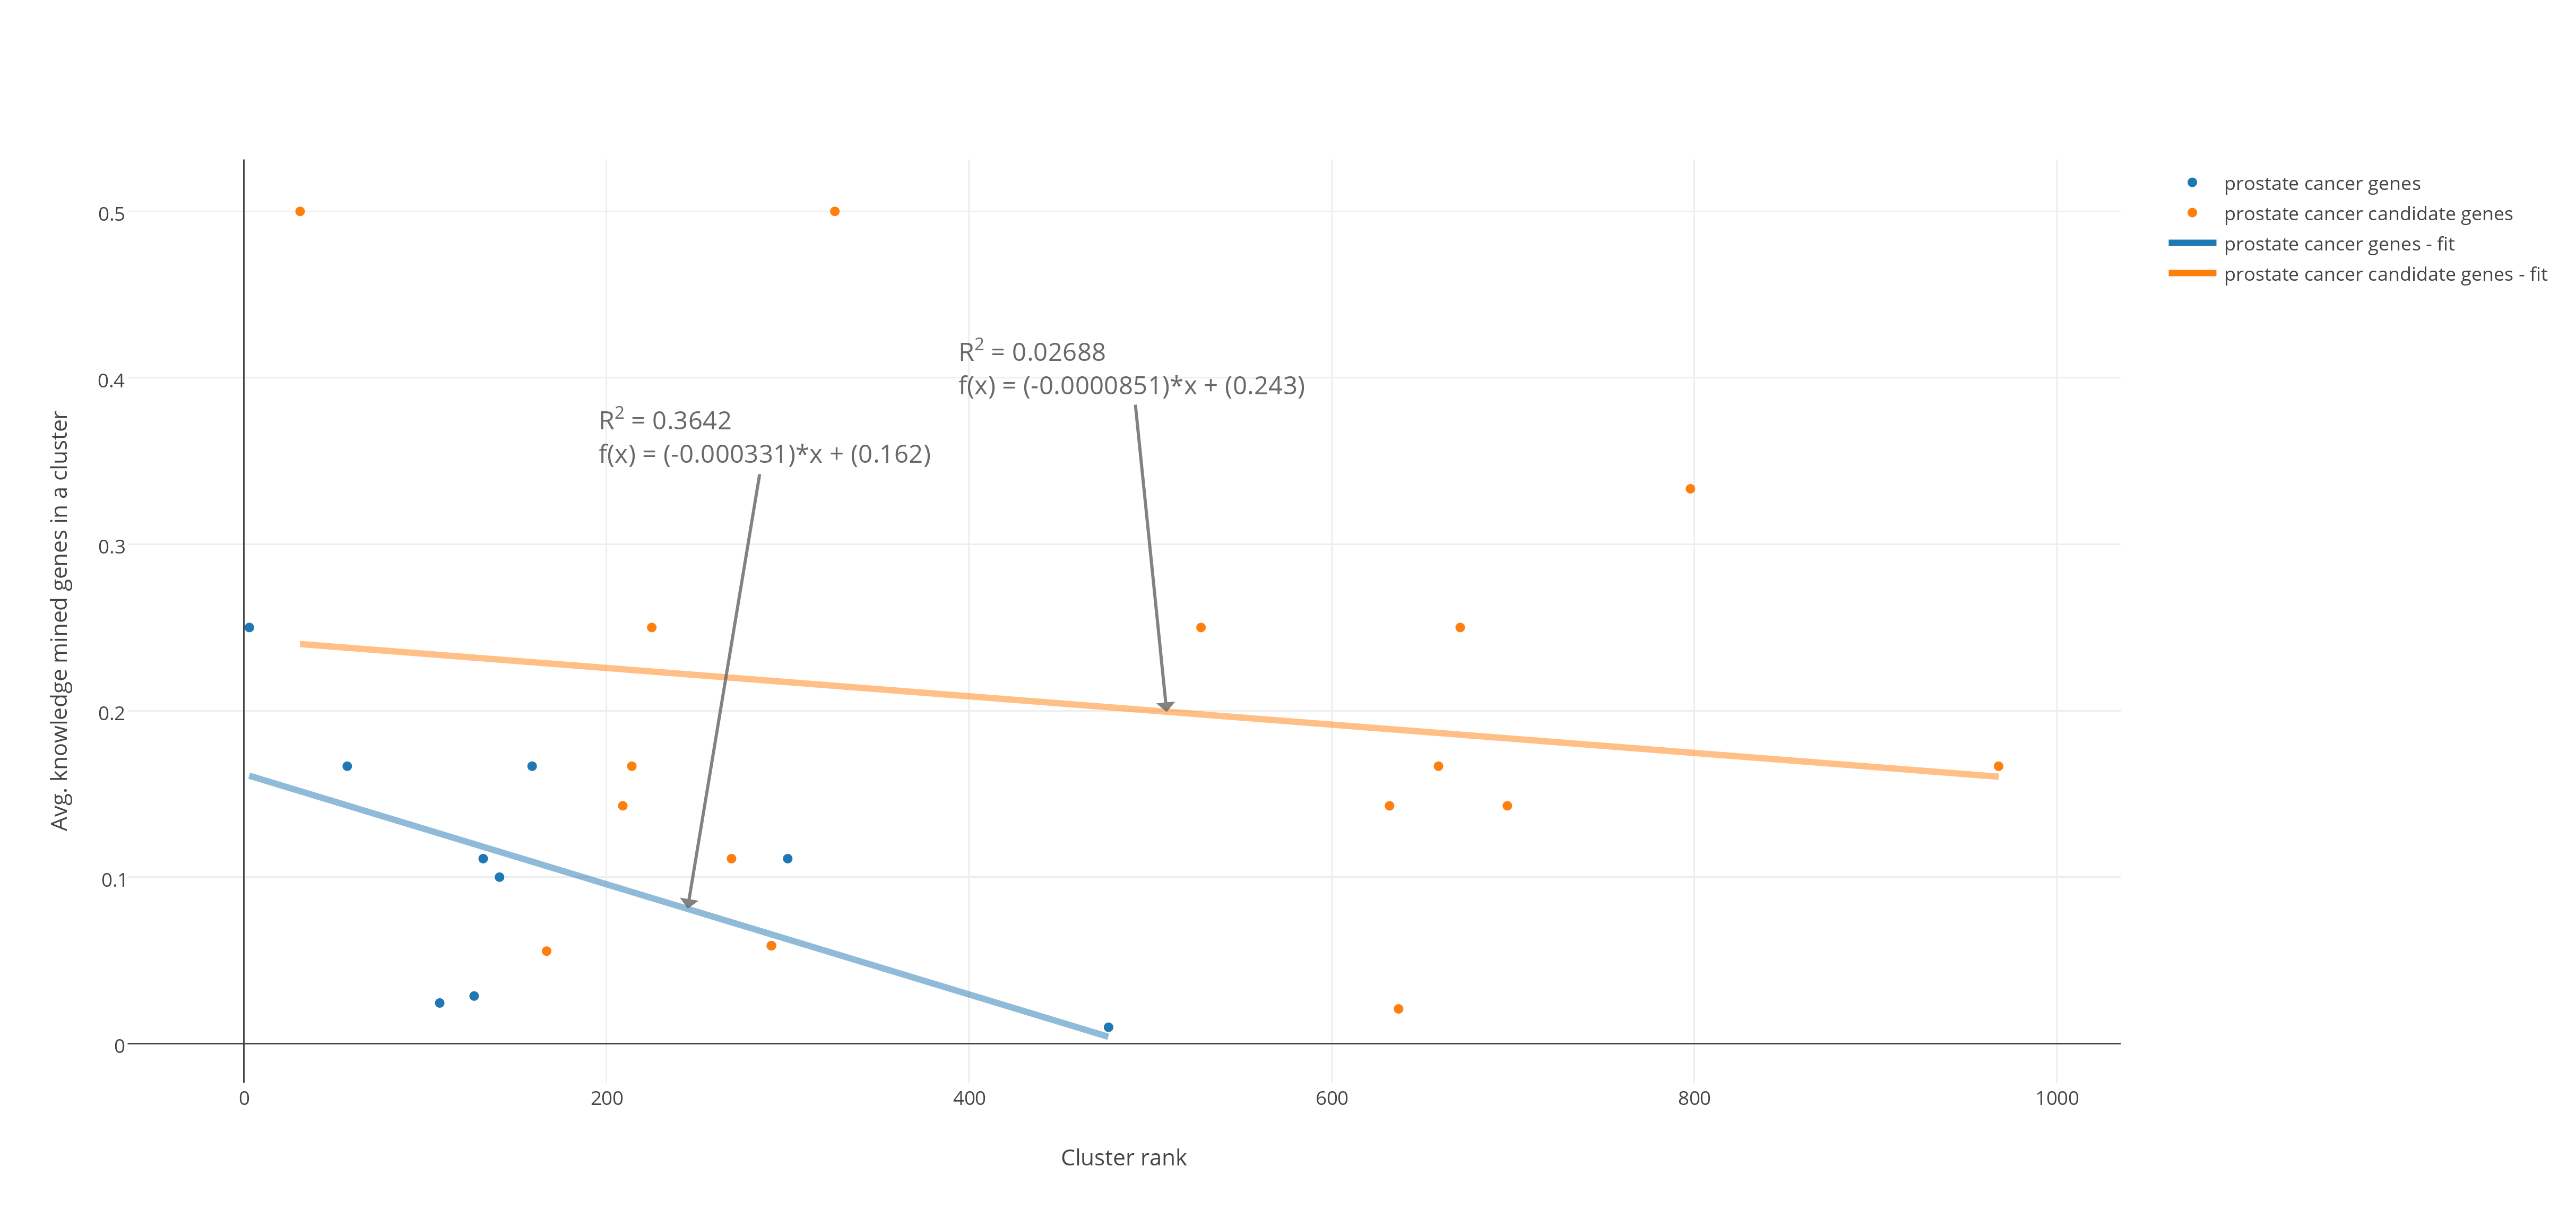
\includegraphics[width=15cm]{prwp_know_split_cosmic}
\end{figure}
\begin{figure}
    \label{fig:exp-cosmic-prwp}
    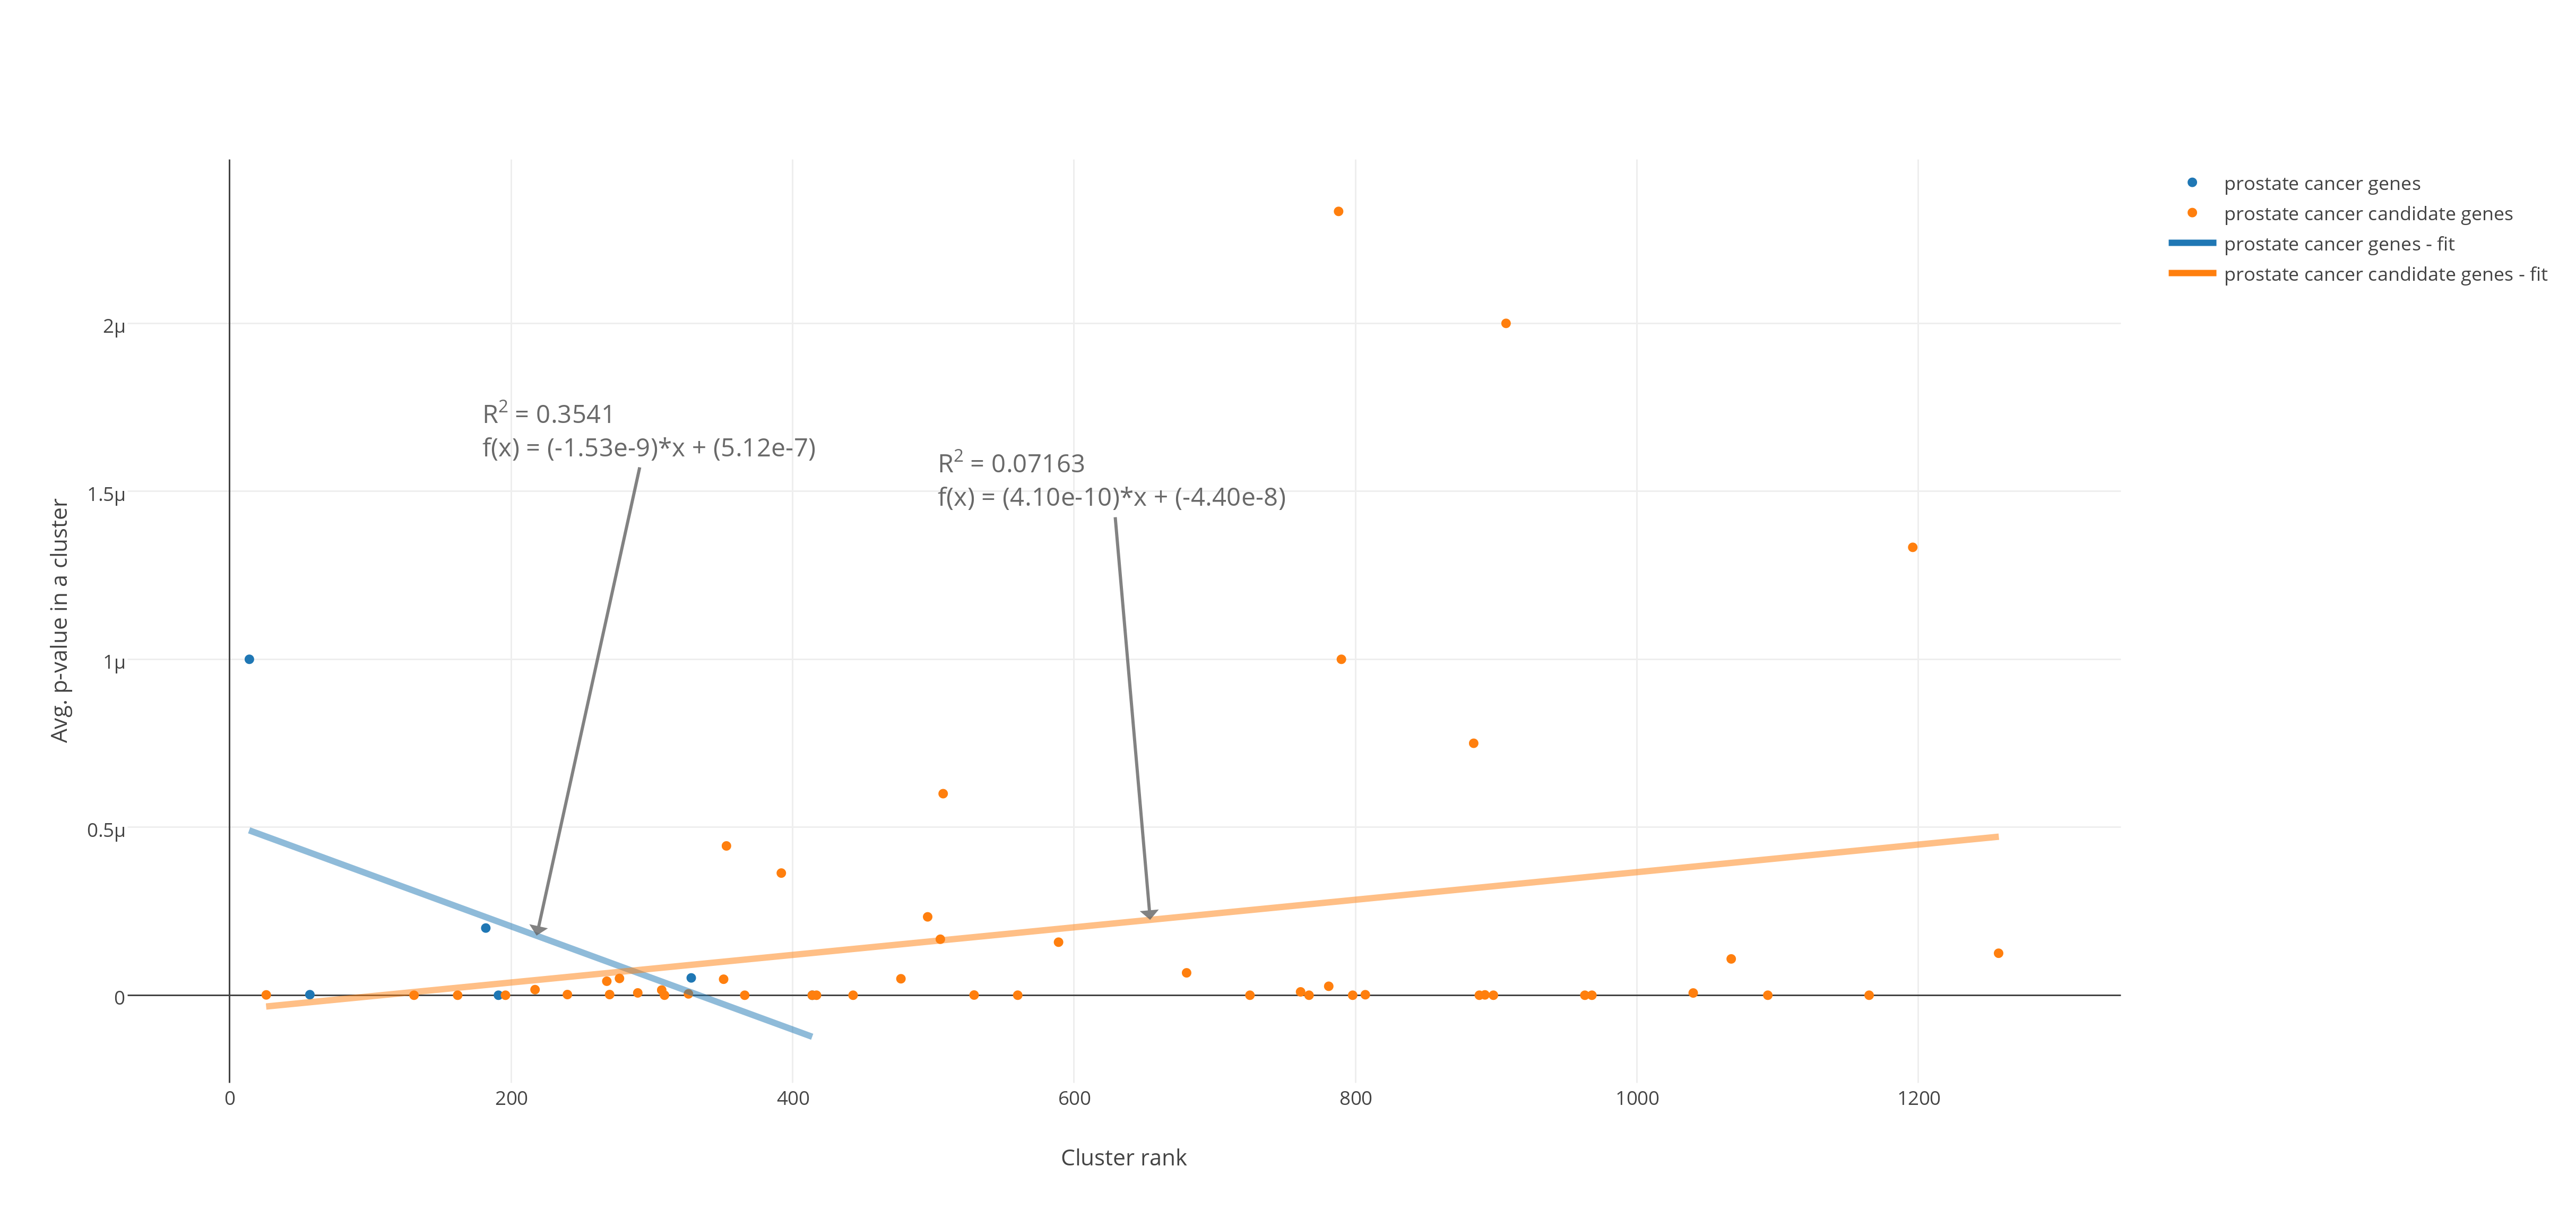
\includegraphics[width=15cm]{prwp_exp_split_cosmic}
\end{figure}

% maa
\begin{figure}
    \label{fig:txt-iref-maa}
    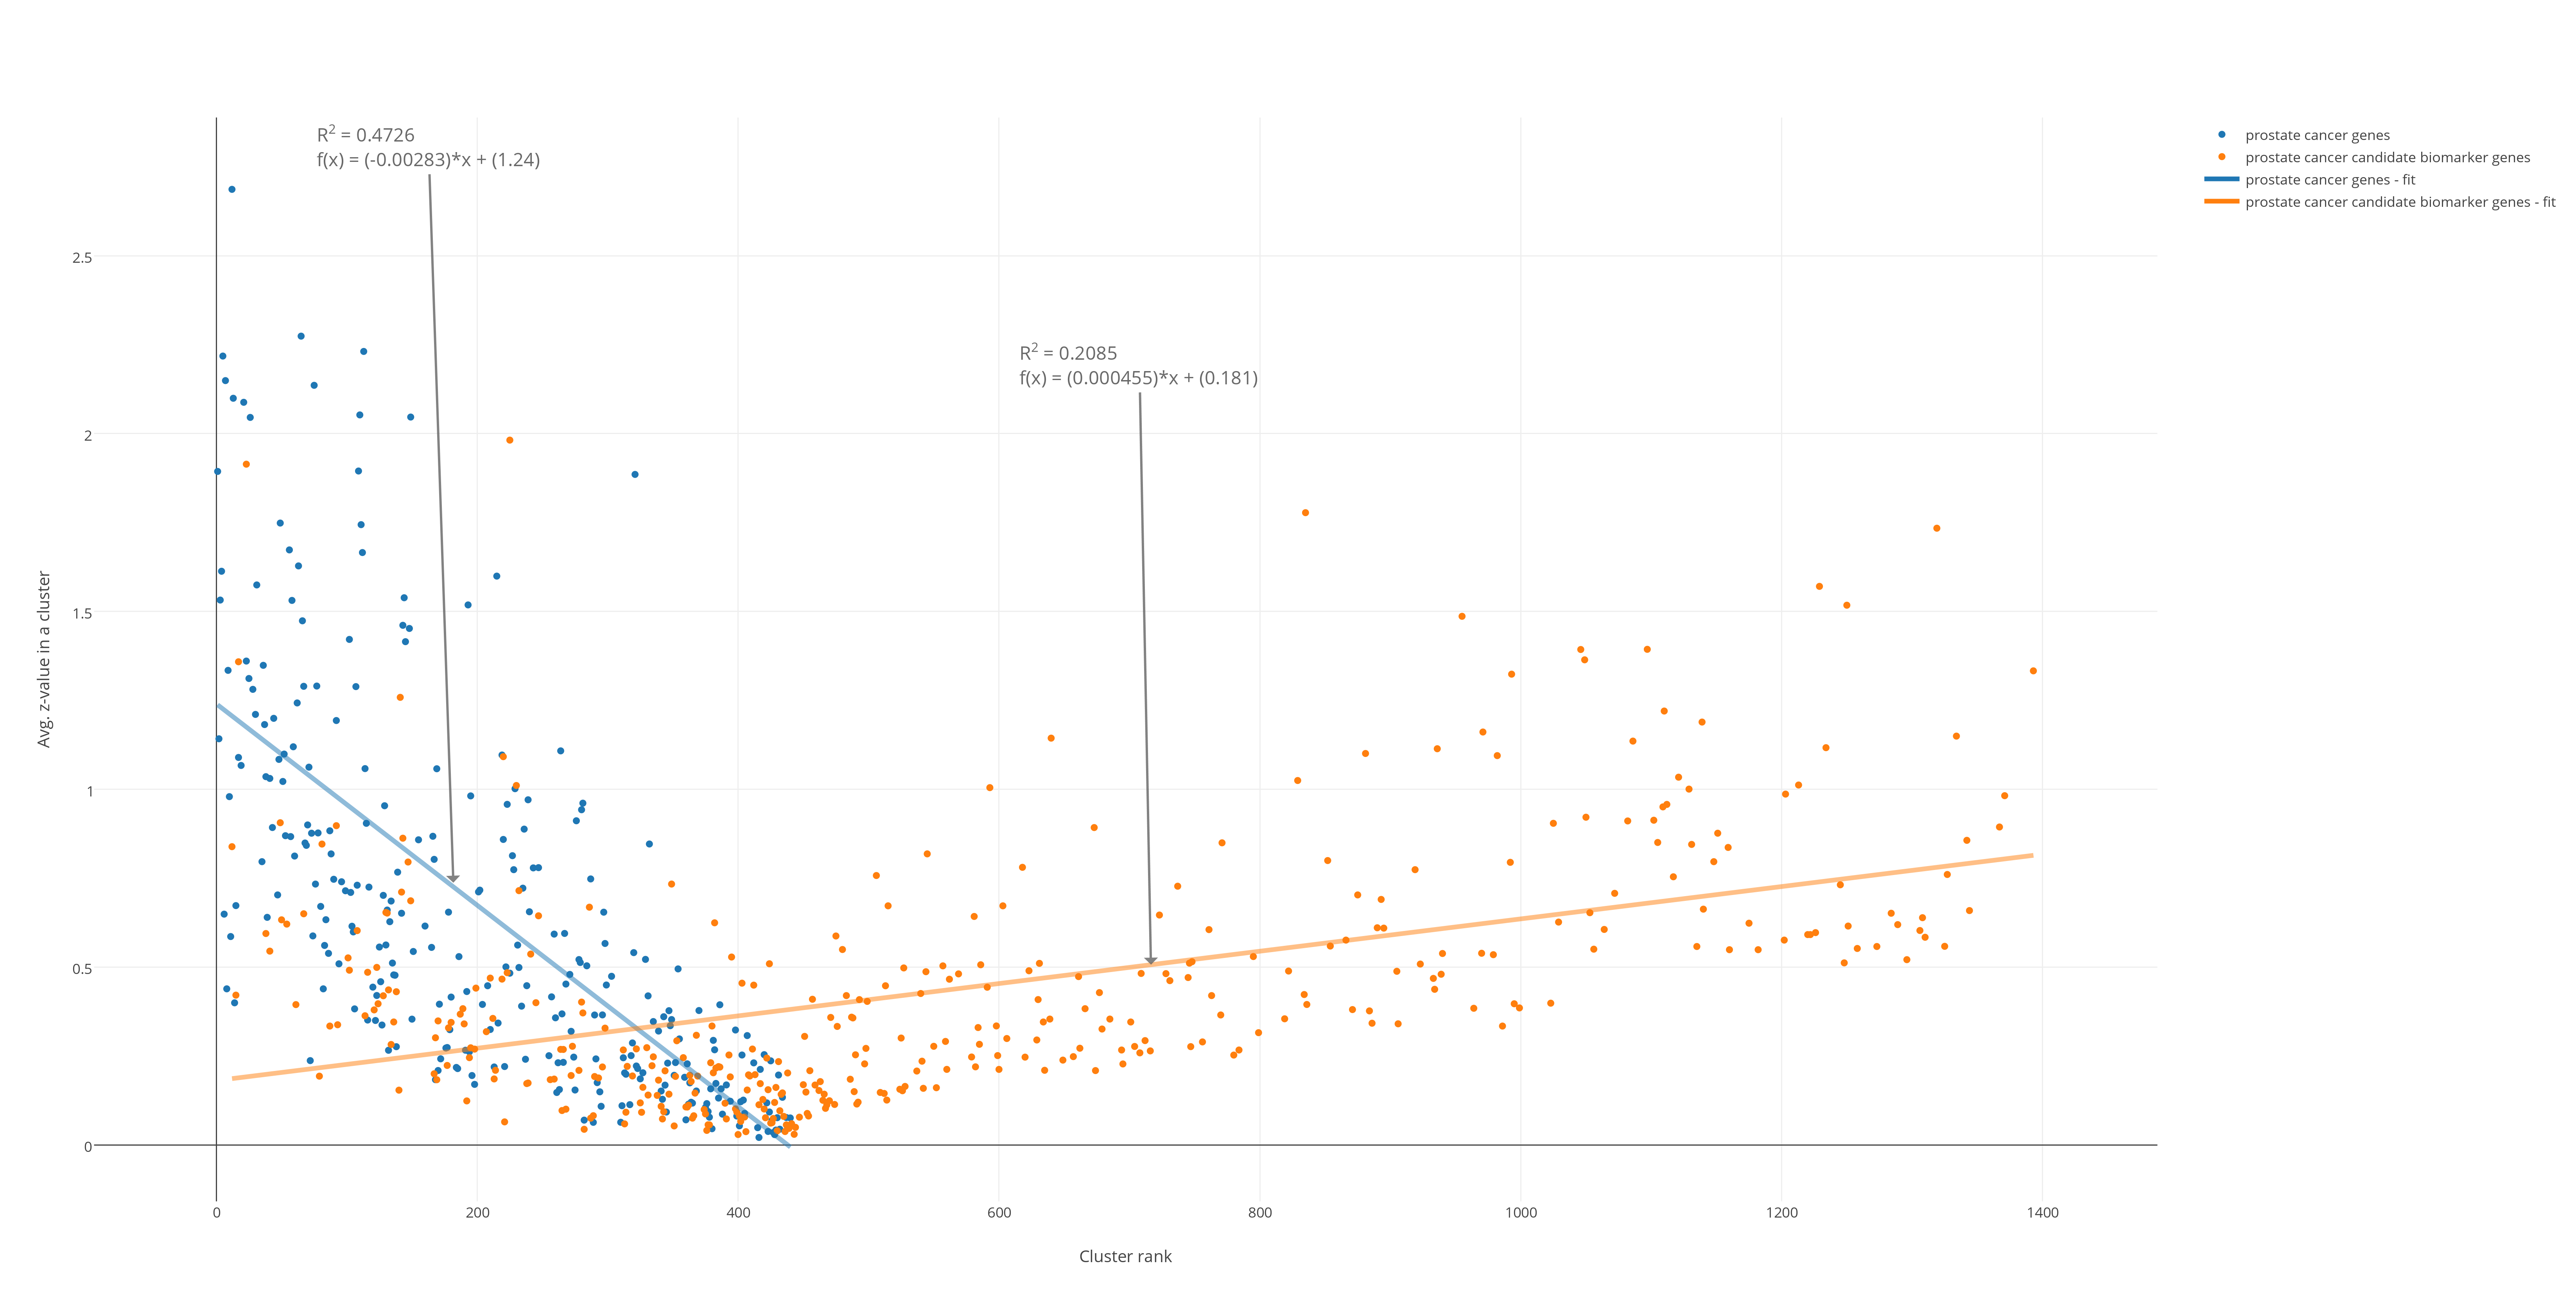
\includegraphics[width=15cm]{maa_textmined_split}
\end{figure}
\begin{figure}
    \label{fig:know-iref-maa}
    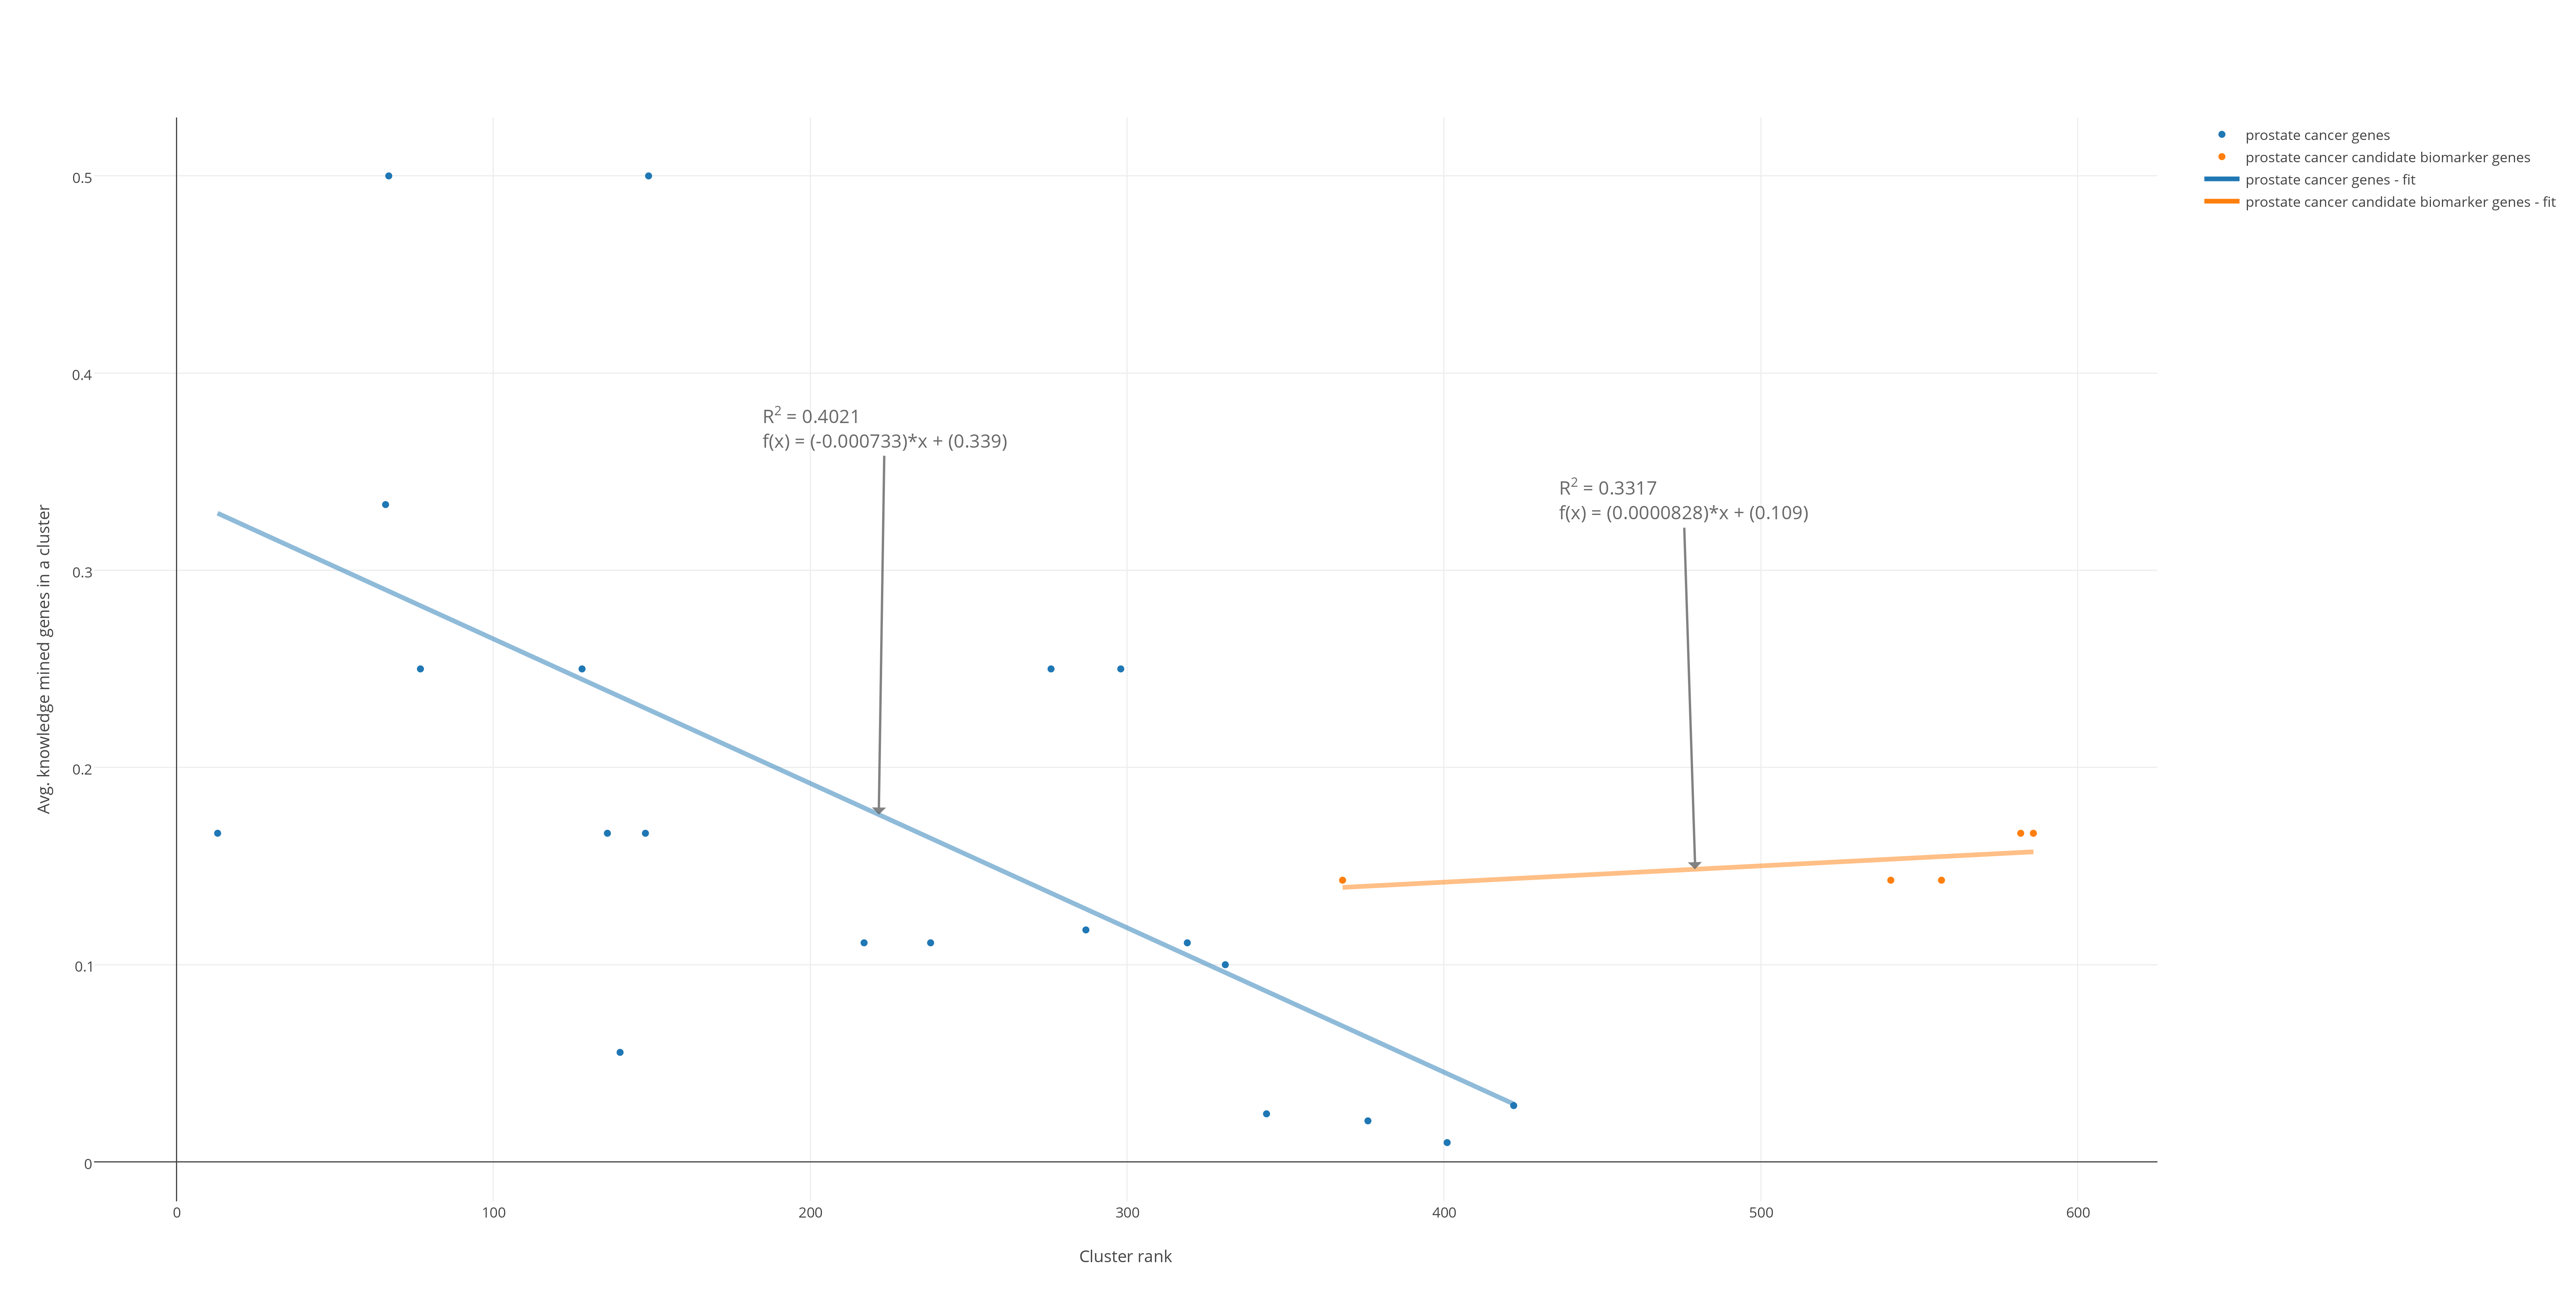
\includegraphics[width=15cm]{maa_knowledge_split}
\end{figure}
\begin{figure}
    \label{fig:exp-iref-maa}
    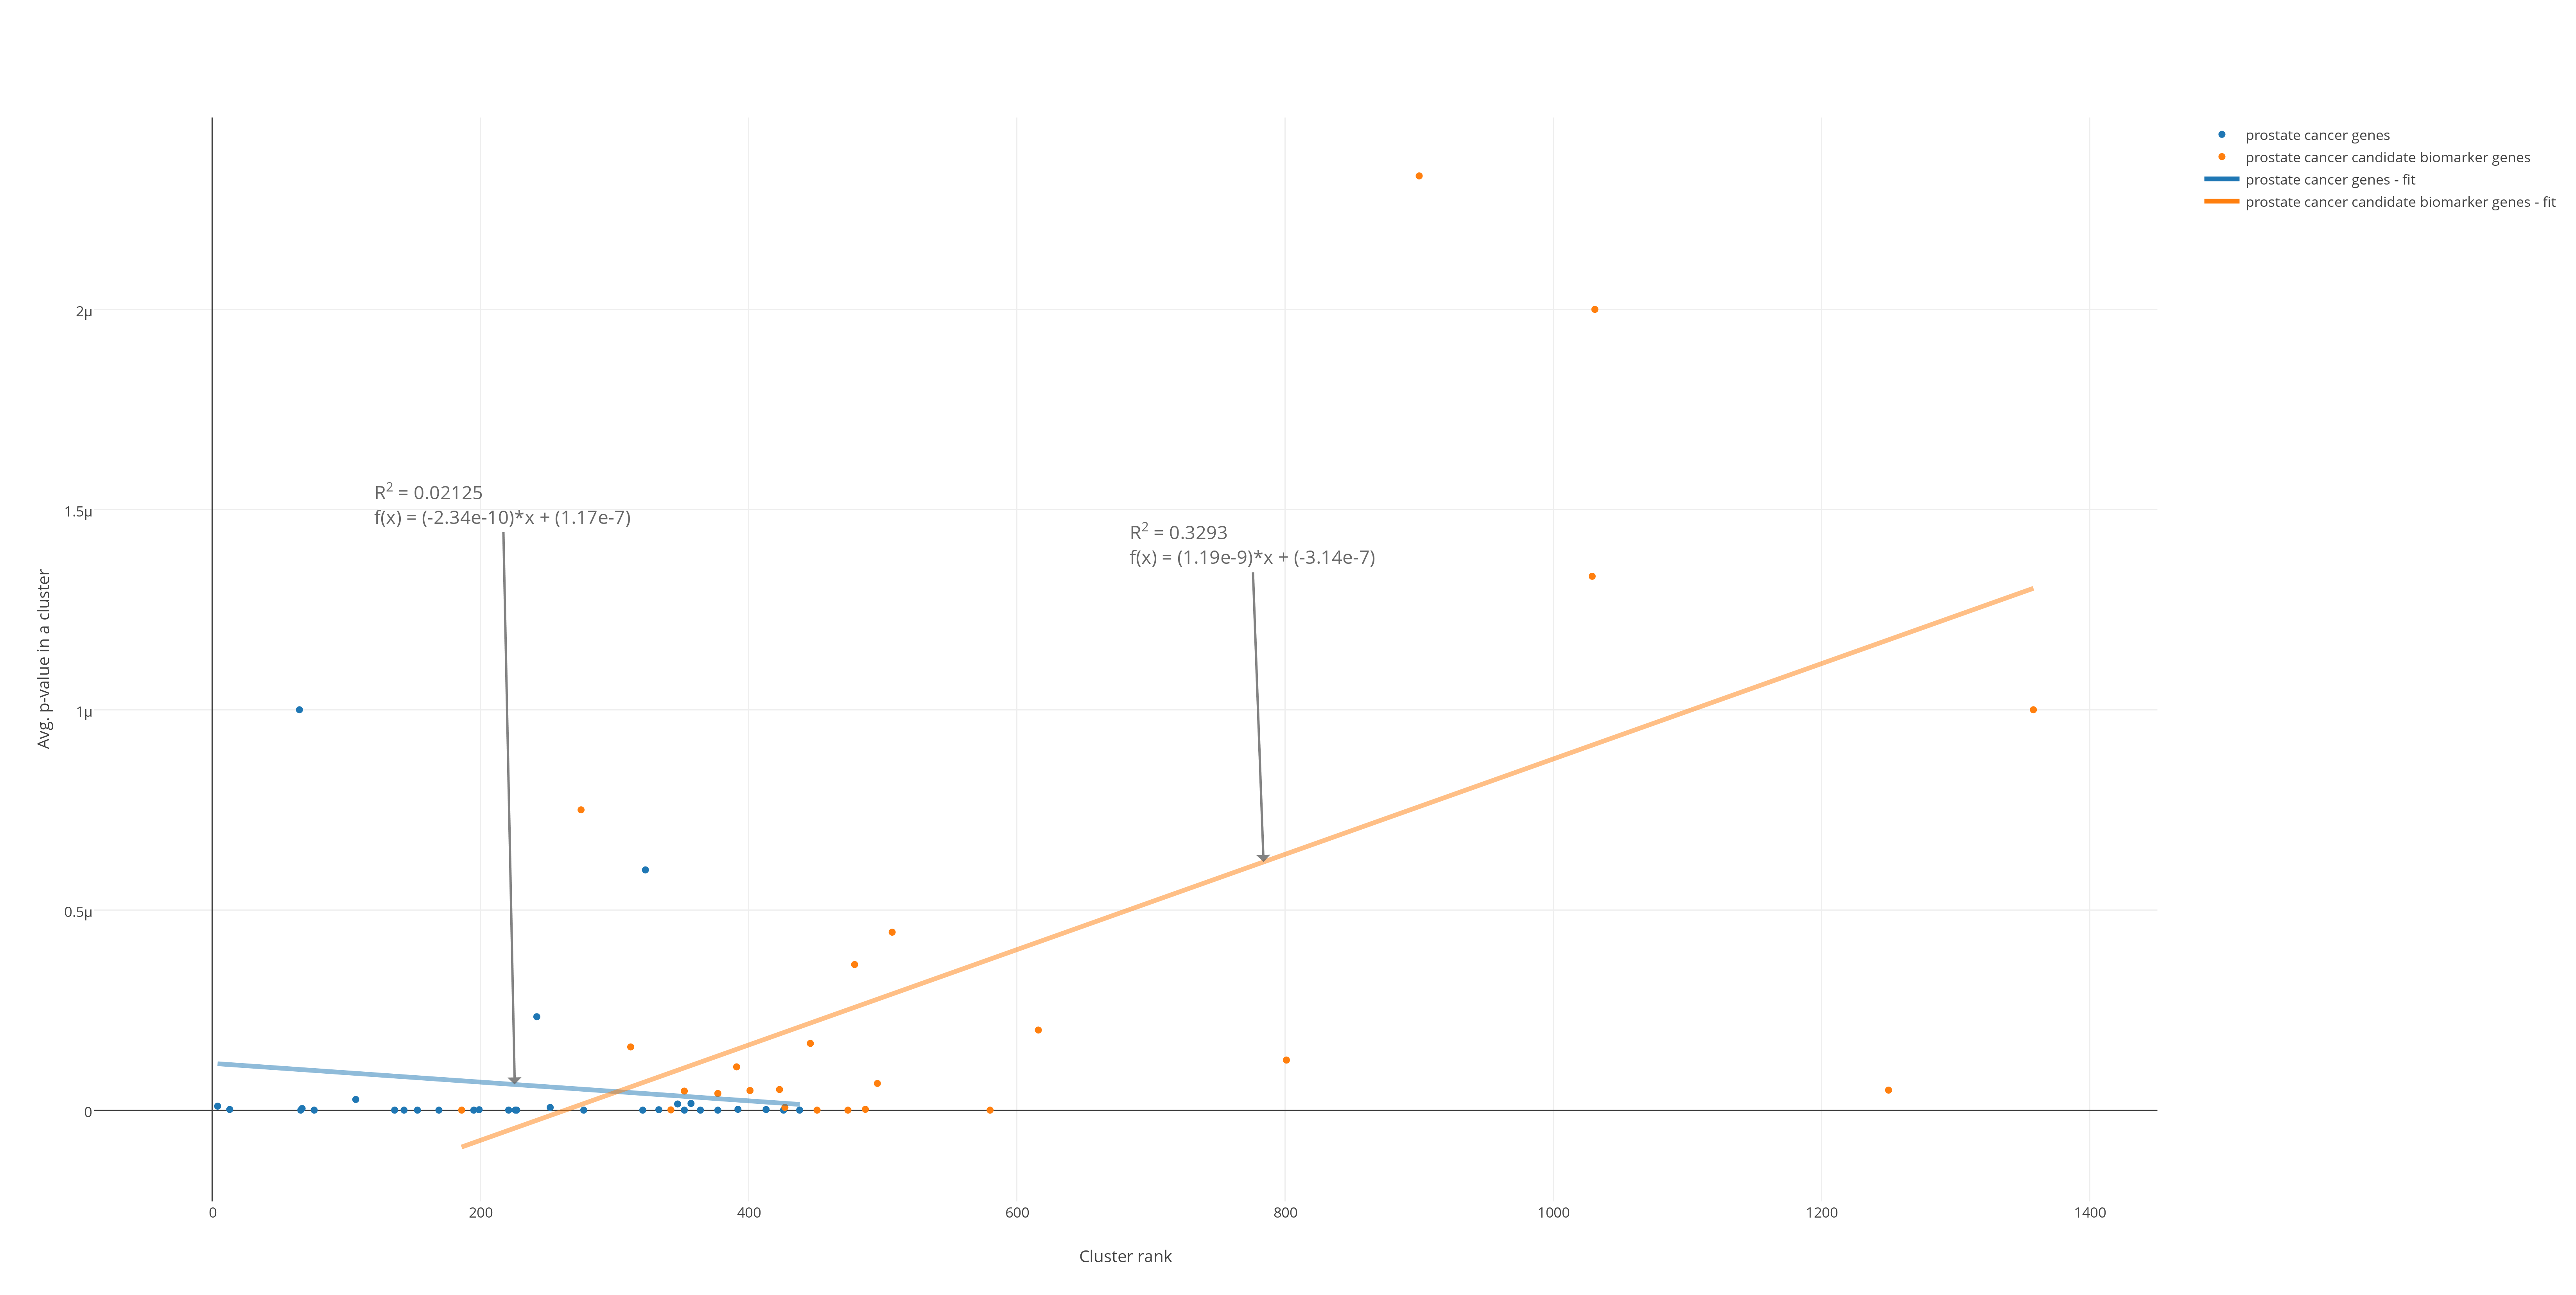
\includegraphics[width=15cm]{maa_experimental_split}
\end{figure}
\begin{figure}
    \label{fig:txt-cosmic-maa}
    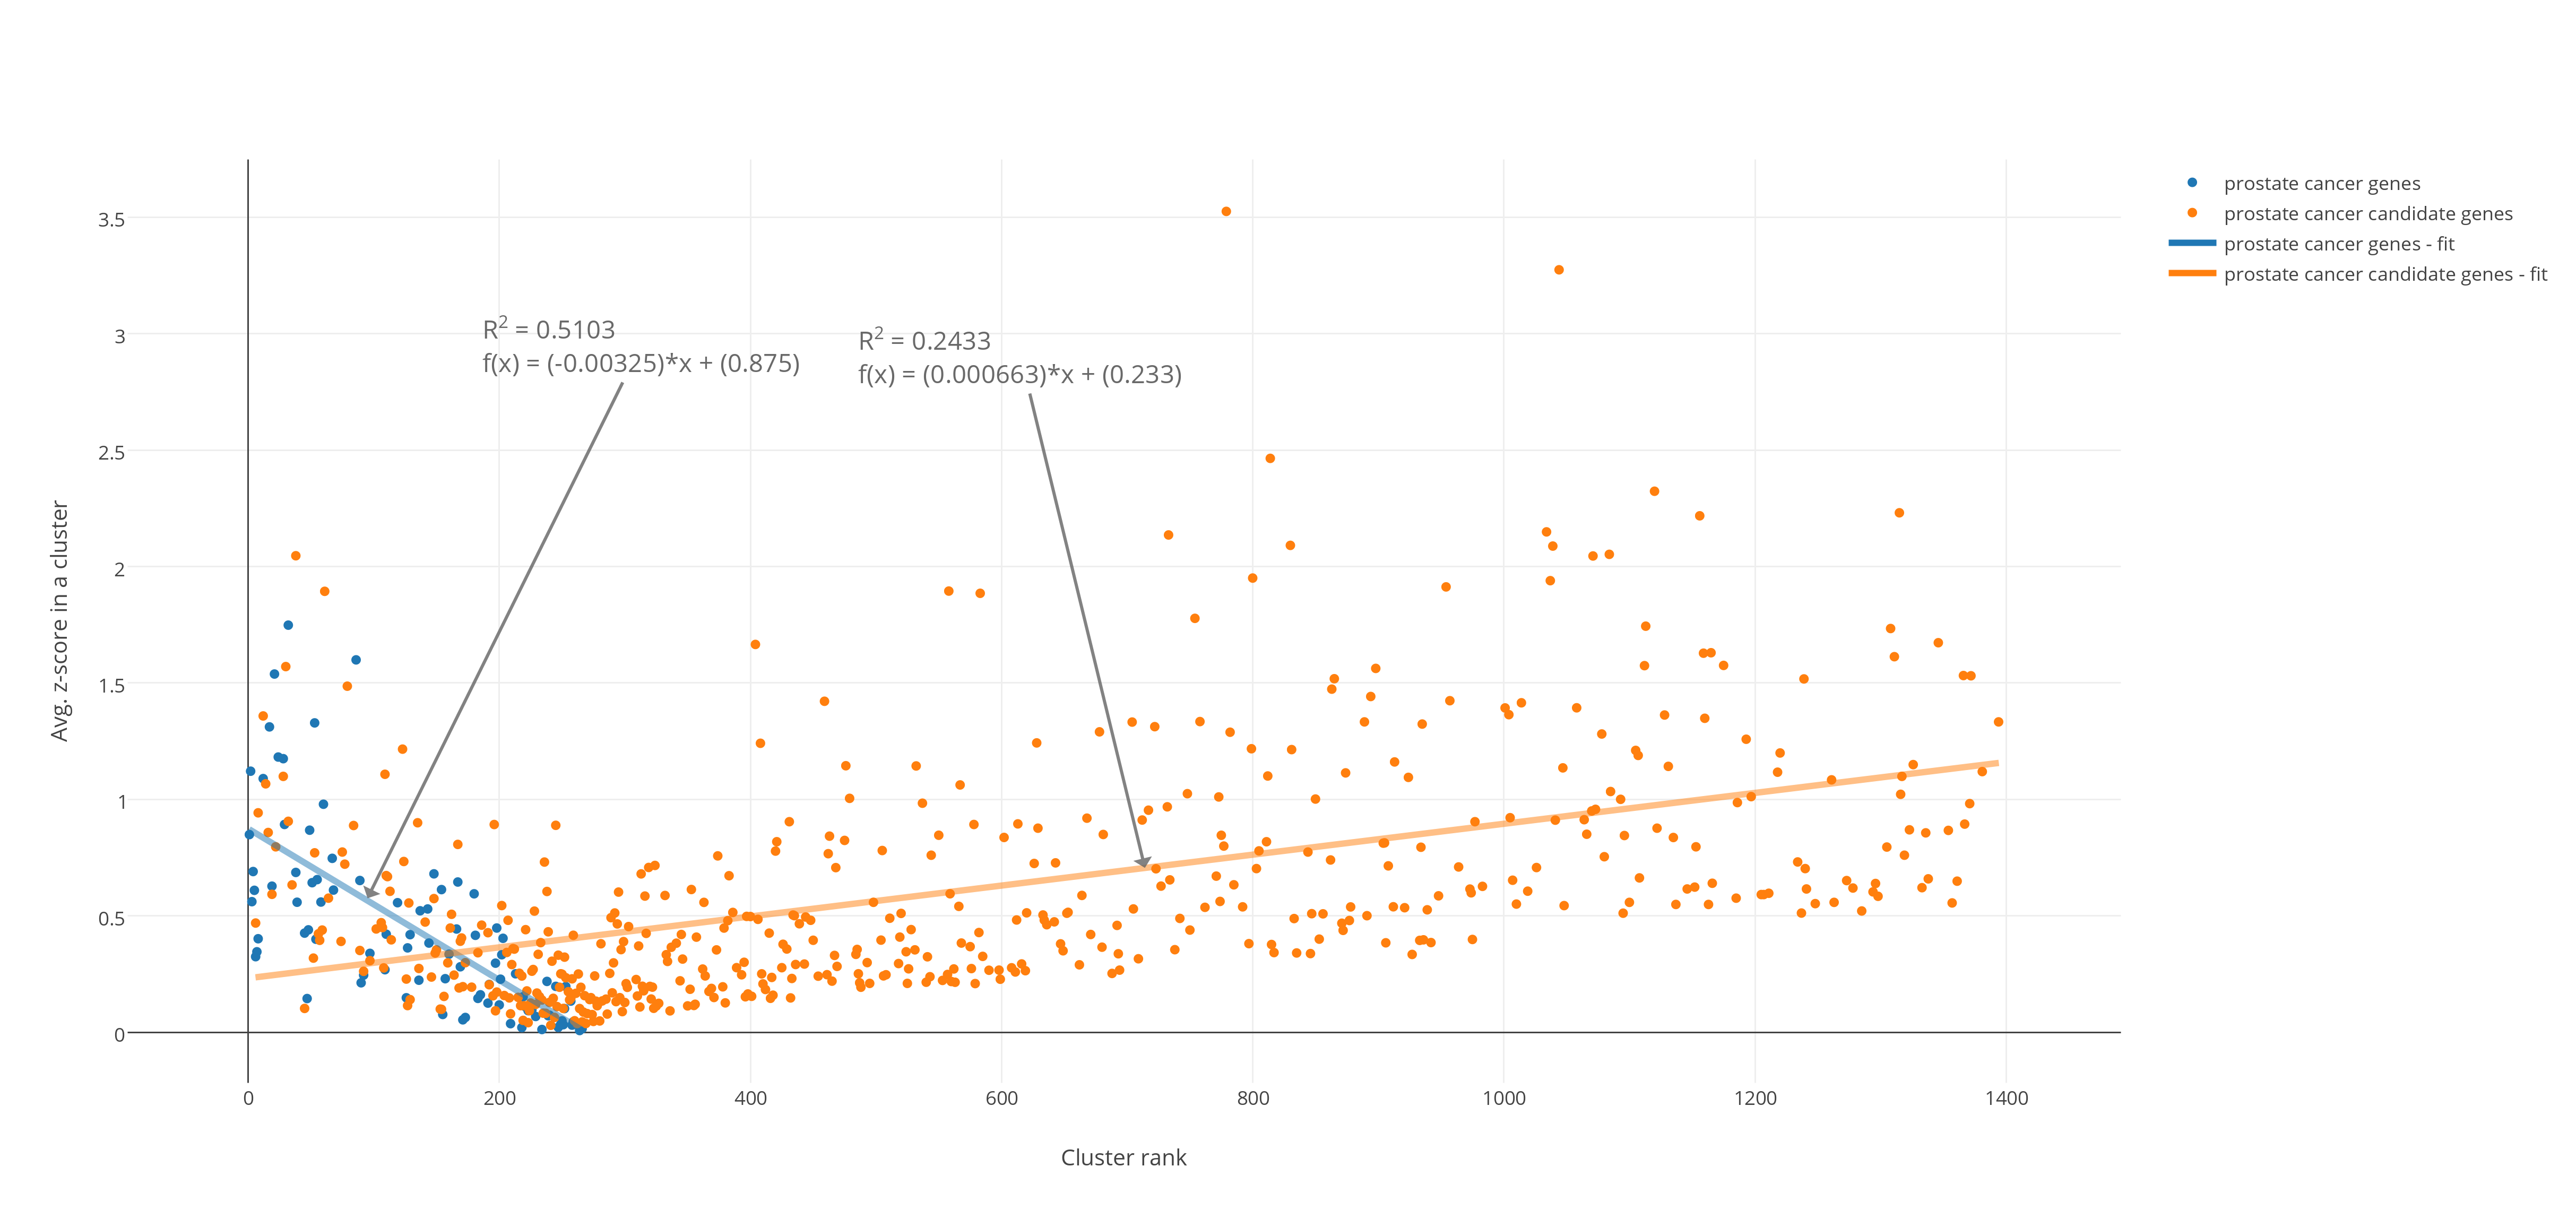
\includegraphics[width=15cm]{maa_txt_split_cosmic}
\end{figure}
\begin{figure}
    \label{fig:know-cosmic-maa}
    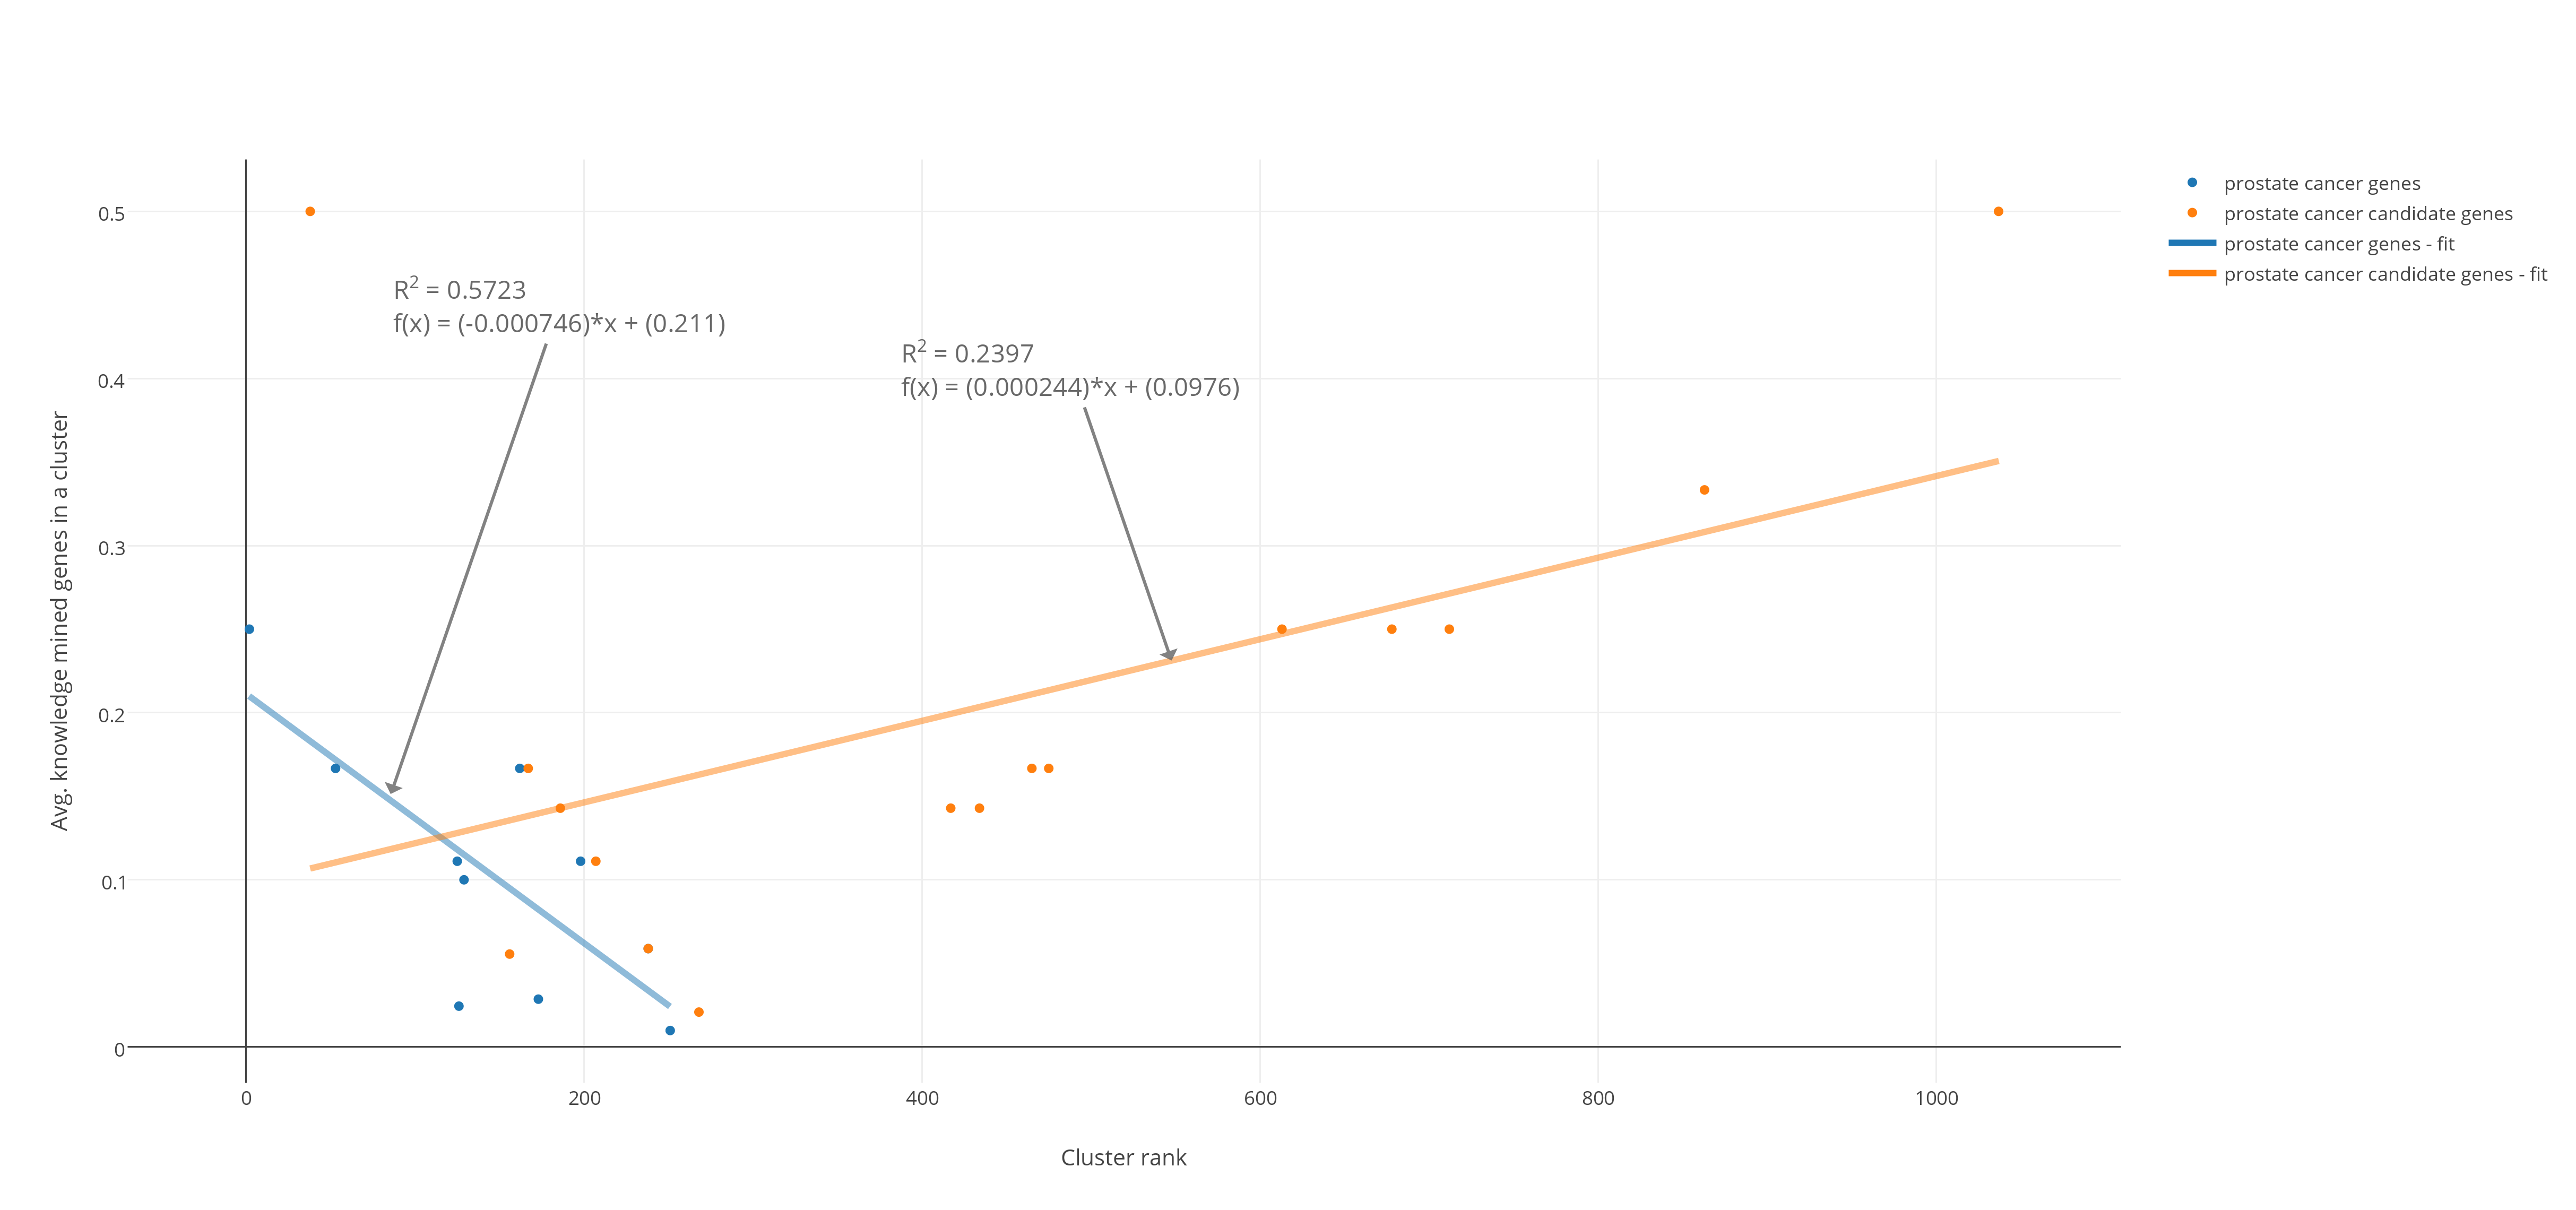
\includegraphics[width=15cm]{maa_know_split_cosmic}
\end{figure}
\begin{figure}
    \label{fig:exp-cosmic-maa}
    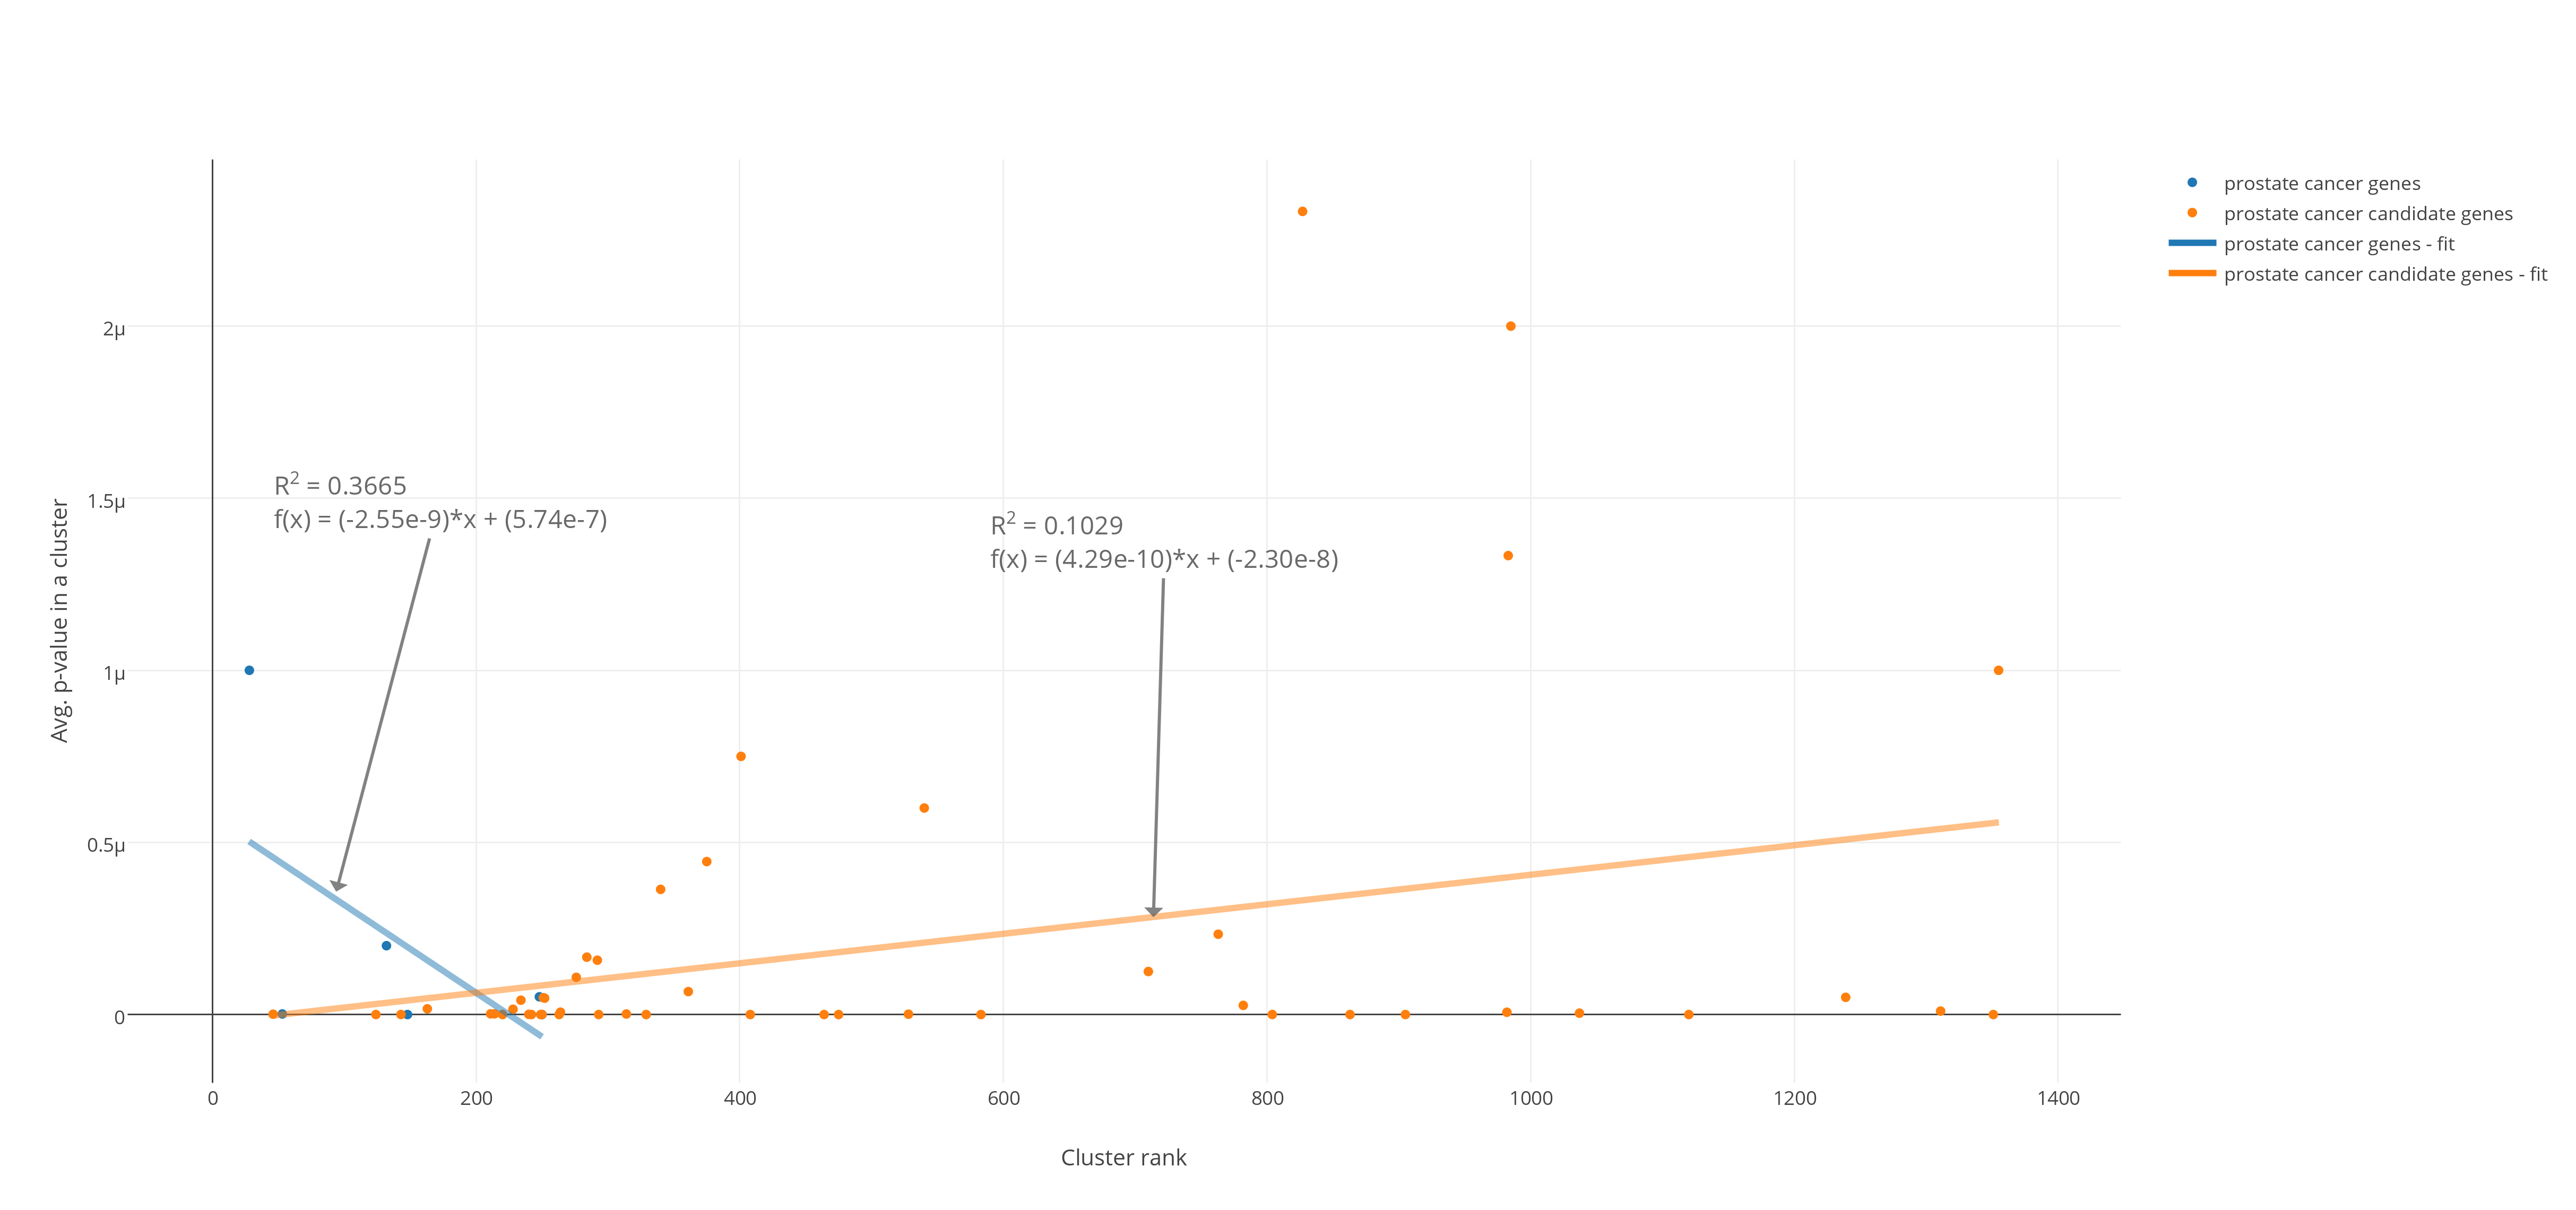
\includegraphics[width=15cm]{maa_exp_split_cosmic}
\end{figure}

\section{Comparison to known biomarkers}
\section{Identification of possible biomarkers}
